\documentclass[11pt]{article}
\renewcommand{\baselinestretch}{1.2} 
\renewcommand{\thefootnote}{\alph{footnote}}
\setlength{\parskip}{2em}
\usepackage[english]{babel}
\usepackage[utf8]{inputenc}
\usepackage{fancyhdr, amsmath,booktabs,mathtools, etoolbox,parskip,
setspace,amssymb,amsfonts,tabularx,graphicx,color,enumitem,tocloft}
\usepackage[hidelinks]{hyperref}

\usepackage[backend=bibtex,
                       sorting=none,
                       citestyle=numeric-comp,
                       bibstyle=chem-acs,
                       firstinits=true]{biblatex}

\usepackage[font={small,stretch=1.1},labelfont=bf]{caption}
\usepackage[bottom]{footmisc}
\graphicspath{ {figures/} }
\usepackage[a4paper, total={6.5in, 9in}]{geometry}
\numberwithin{equation}{subsection}

\pagestyle{fancy}
\fancyhf{}
\rhead{SI: Reaction Dynamics of Diels-Alder Reactions from Machine Learned Potentials}
\cfoot{\thepage}

% Custom commands
\newcommand{\kcal}{kcal mol$^{-1}$}
\newcommand{\tacc}{$\tau_\text{acc}$}
\newcolumntype{Y}{>{\centering\arraybackslash}X}
\newcolumntype{C}{>{\centering\footnotesize}X}

\newcommand{\comment}[1]{}

% Redefine numbering in the SI
\renewcommand{\thepage}{S\arabic{page}}
\renewcommand{\thesection}{S\arabic{section}}
\renewcommand{\thetable}{S\arabic{table}}
\renewcommand{\thefigure}{S\arabic{figure}}
	
\bibliography{refs}

% Make the Table of Contents numbering not overlap
\addtolength{\cftsecnumwidth}{5pt}

\begin{document}	
\begin{titlepage}
	\vspace*{\fill}
	\begin{center}
		{\huge \bfseries{Supporting Information}}\\
		\vspace{0.2cm}
		{\huge Reaction Dynamics of Diels-Alder Reactions from Machine Learned Potentials}\\
		\vspace{0.2cm}
		{Tom A. Young, Tristan Johnston-Wood, Hanwen Zhang and Fernanda Duarte}
	\end{center}
	\vspace*{\fill}

\end{titlepage}	
\newpage

\tableofcontents
\clearpage


\section{Methods} \label{section::SI_methods}

All Gaussian Approximation Potentials (GAPs) were trained using the gap\_fit and QUIP codes with a Smooth Overlap of Atomic Positions (SOAP)\cite{Bartk2013} kernel with hyperparameters as defined in Table \ref{table::SX1}. GAP-MD simulations were performed with ASE\cite{HjorthLarsen2017} interfaced to QUIP with the quippy wrapper using the Langevin integrator. Initial configurations, CUR\cite{Mahoney2009} selection and automated training set construction were generated with the mltrain Python package (v. 1.0.0a).\cite{Young2021mlt} Training sets for initial GAPs including those that used GP variance as a selection criteria were constructed using the gap-train code (v. 1.0.0b).\cite{Young2021gt} ACE\cite{Kovacs2021, Drautz2019} potentials were trained using the ACE.jl code\cite{Ortner_ACE} (v 0.8.4, Julia v. 1.6.3) and wrapped by pyjulip (v. 0.1, using PyCall). All dynamics were propagated using the Langevin (0.02 friction coefficient) integrator in ASE v. 3.22.0 with initial velocities sampled from a Maxwell-Boltzmann distribution then propagated using a 0.5 fs timestep. NequIP\cite{Batzner2021} potentials used the nequip\cite{nequip_github} v. 0.3.3 Python package (pytorch v. 1.9.1, pytorch\_geometric v. 1.7.2, e2nn\cite{e3nn} v.0.3.5) with a maximum 1000 epochs and a 90:10 training to validation data split; all other hyperparameters were retained as their defaults (4.0 \AA~cut off radius, see nequip module in ml-train, commit 0ba027c). Gas phase (vacuum) simulations in periodic potentials used a large cubic box ($l = 10$ nm). Combinations of harmonic restraining potentials were added and incorporated into the dynamics using ASE. Ring polymer molecular dynamics simulations were performed using I-PI\cite{Kapil2019} with 16 beads, a 0.5 fs timestep, 300 K either default NVT (Langevin) or NVE dynamics. 

DFTB calculations were performed with DFTB+\cite{Hourahine2020} using 3ob\cite{Gaus2014} parameters in a periodic box with side lengths of 50 \AA~to mimic a vacuum. Molecular DFT used GFN2-XTB\cite{Bannwarth2019} in XTB v. 6.4.0. Molecular DFT (inc. AIMD), MP2 and coupled cluster [CCSD(T)] calculations performed with ORCA\cite{Neese2017, Neese2020} v. 4.2.1 wrapped with autodE\cite{autodE} using PBE\cite{Perdew1996} and PBE0\cite{Adamo1999} functionals, def2-SVP, def2-TZVP, def2-TZVPP basis sets.\cite{Weigend2005} DLPNO coupled cluster calculations employed TightPNO thresholds.\cite{Yang2018} Double-hybrid DFT calculations were performed in ORCA v. 5.0.2. Transition states were located with autodE. Plots were generated with matplotlib and, where quoted, include a standard error of the mean averaged over three independent repeats.


\section{Author Contributions}
X
{\huge{TO WRITE}}


\clearpage
\section{GAPs for Reactions} \label{section::SI_gap_reactions}

Using our initial GAP training strategy,\cite{gaptrain2021} found to be effective for developing an accurate reactive potential for the S${}_N$2 reaction Cl${}^{-}$ + CH${}_3$Cl in the higher-dimensional ethene+butadiene Diels-Alder case did not afford a chemically accurate GAP (\figurename{ \ref{fig::SX30}a}). However, for a similarly complex H-abstraction reaction the obtained error is closer to the target 1 \kcal~(0.04 eV) level of accuracy (\figurename{ \ref{fig::SX30}b}). Note that these results are consistent within repeats of the partially random AL strategy and minor hyperparameter tweaks.


\begin{figure}[h!]
\centering
\vspace{0.4cm}
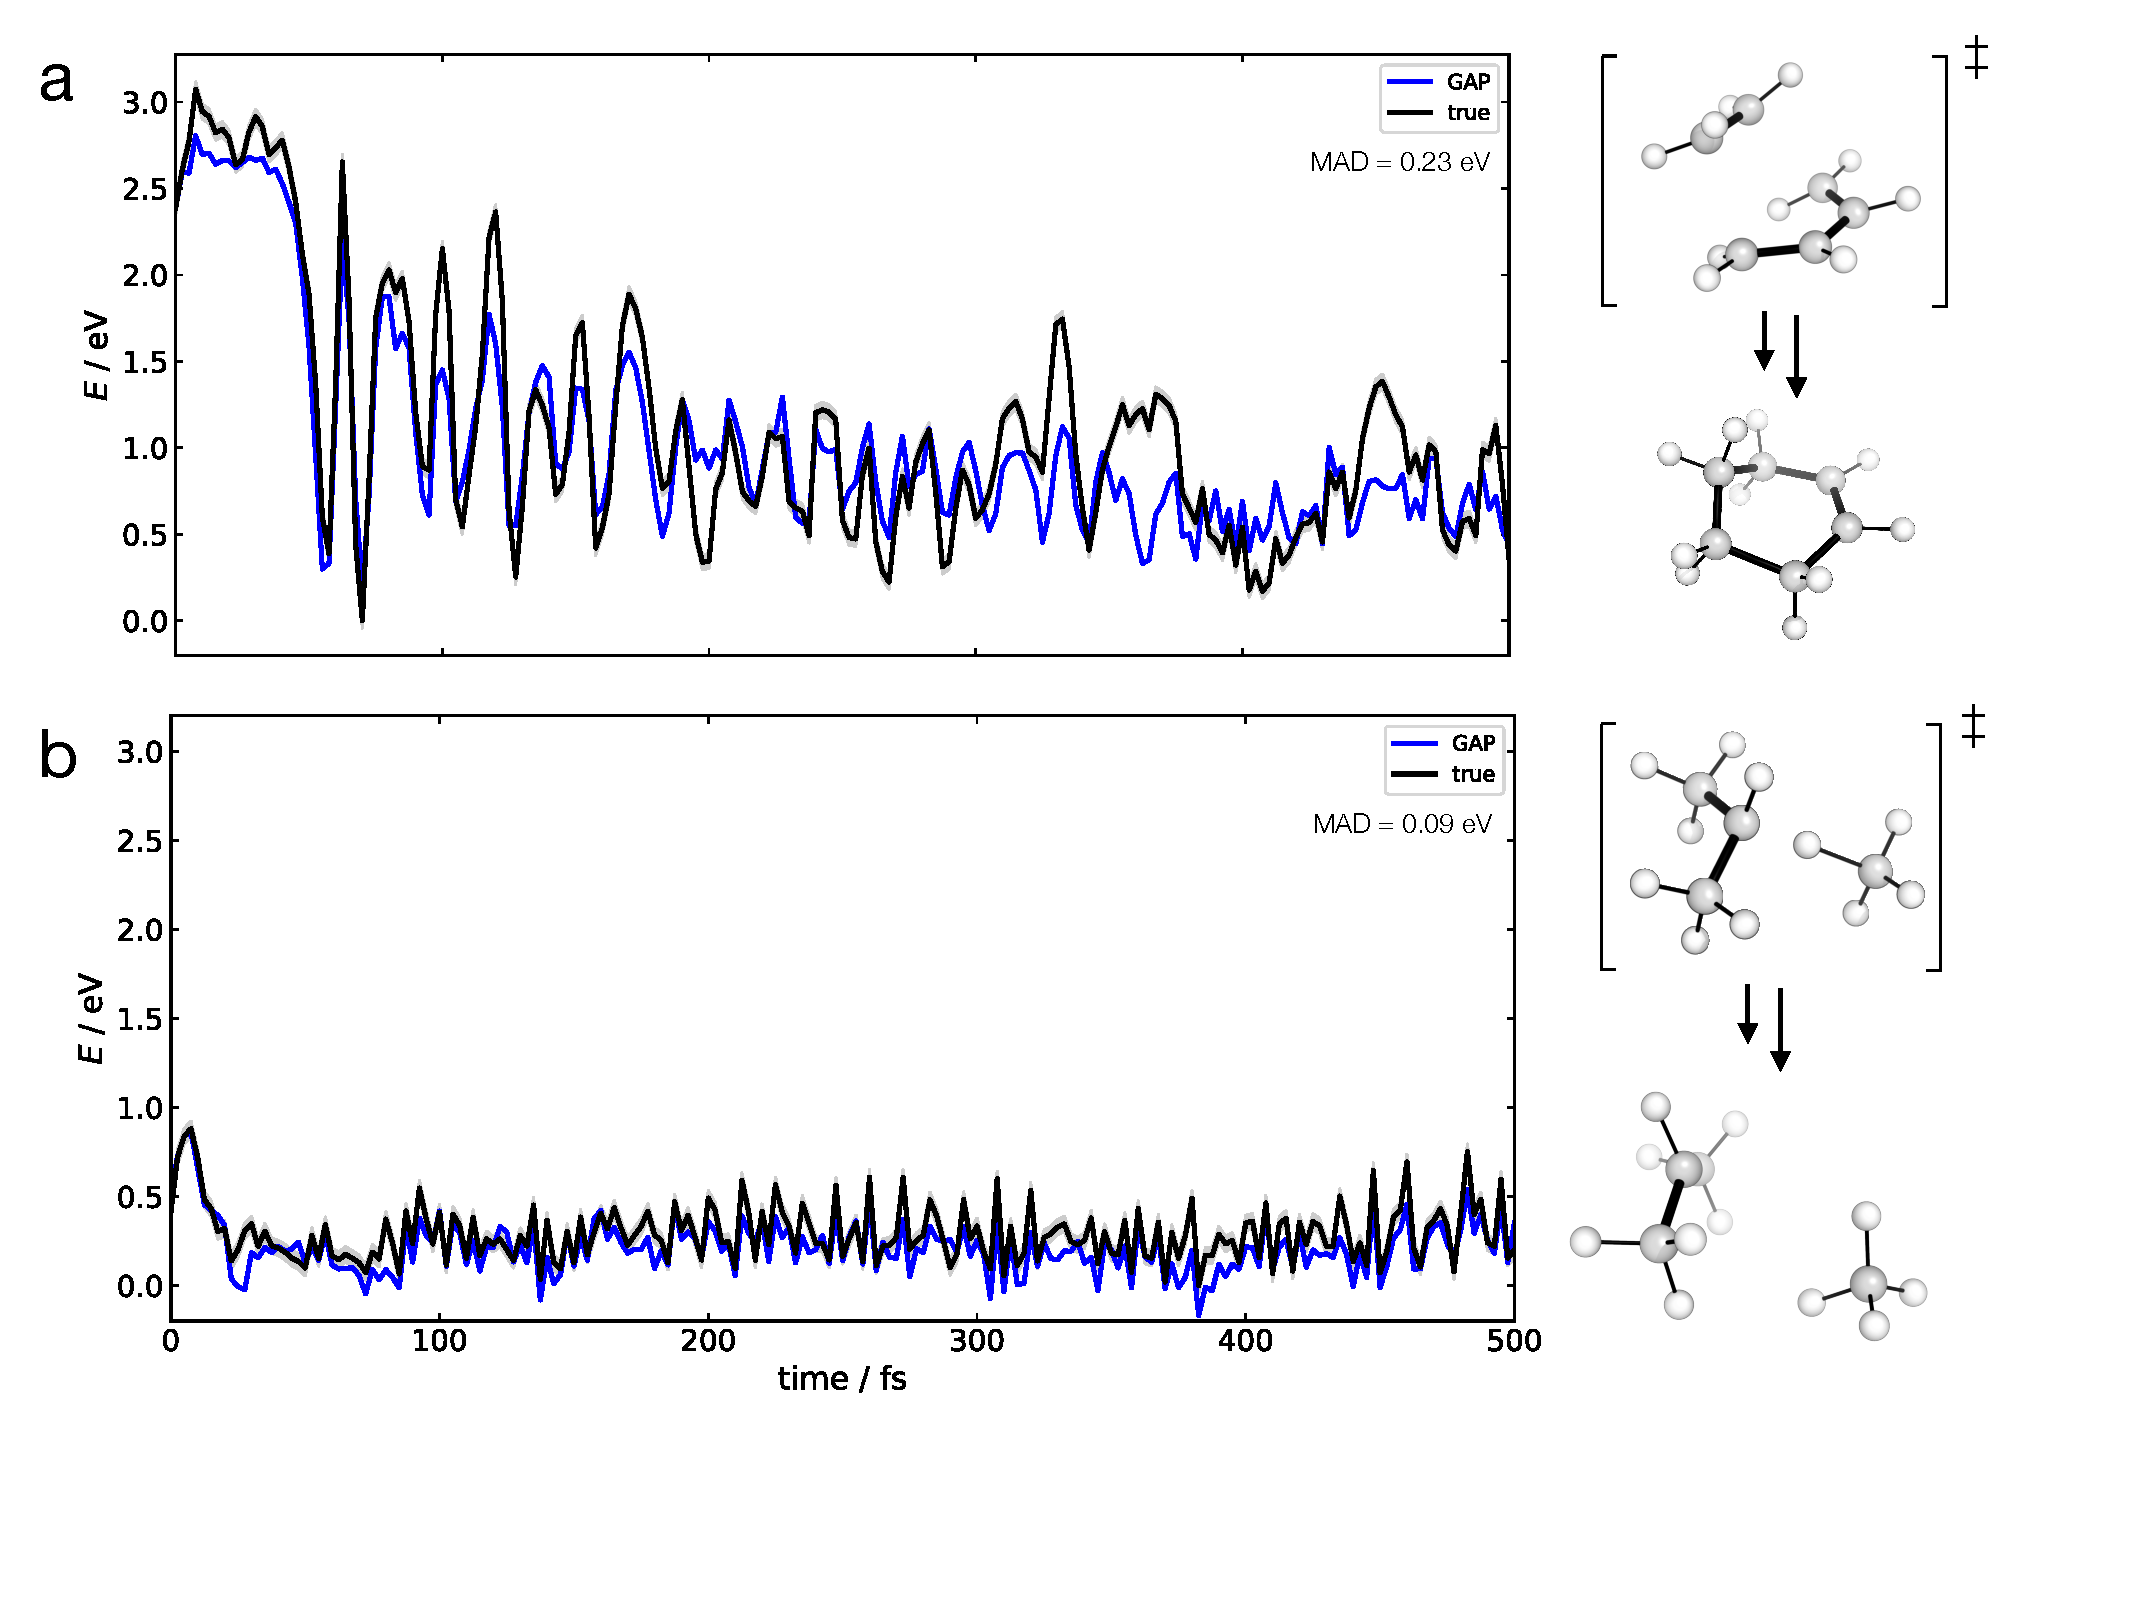
\includegraphics[width=0.9\textwidth]{figSX30.pdf}
\vspace{0.0cm}
\hrule
\vspace{0.1cm}
\caption{Comparison of predicted and true energies over a GAP-MD propagated trajectories using initial velocities suitable for 300 K and a Langevin thermostat (300 K) with a 0.5 fs time step. 'True' energies calculated at PBE0-D3BJ/def2-SVP in ORCA. GAPs trained using active learning (AL) and the same hyperparameters in ref. \cite{gaptrain2021} at 500 K. AL used a $E_T = 2\times10^{-5}$ eV atom${}^{-1}$ threshold on the maximum Gaussian process variance to select new configurations within a 1 ps window. Final datasets contained 217 and 223 configurations for ethene + butadiene (a) and methyl + propane (b) respectively.}
\label{fig::SX30}
\end{figure}



\clearpage
\section{System Size Scaling} \label{section::SI_system_size}

Extending our initial work on a selection of modestly-sized systems and configurational complexity,\supercite{gaptrain2021} the following section outlines the how the number of evaluations are required to train a chemically accurate GAP (over $>1$ ps simulation time) scales with system size (hyperparameters shown in \tablename{ \ref{table::default_params}}, standard active learning methodology described in ref. \cite{gaptrain2021}).
\vspace{0.3cm}

\begin{table}[h!]
	\def\arraystretch{1.3}
	\begin{tabularx}{\textwidth}{YYCY}
		\hline
		Type&	Parameter	& Description &Value\\
		\hline
			 GAP	   &  $\sigma_E$	&Expected error in energies&        0.316 meV  atom$^{-1}$\\
			               &   $\sigma_F$&	Expected error in force components&  	0.1 eV \AA${}^{-1}$
		\\
		                  & $\zeta$         &Power the kernel is raised to, increasing the dissimilarity between environments ($\zeta > 1$)& 	4
		\\
		                  & $n_\text{sparse}$	     & Number of atomic environments above which  selection is performed &500
		\\
		
		&sparse method	& Method to select the maximumly diverse set of configurations &CUR points\\
		&&&\\
		SOAP descriptors  &$\sigma_\text{at}^\text{SOAP}$& Spread of the Gaussian added to each nuclear coordinate&0.5 \AA
		\\
		                   &$n_\text{max}, l_\text{max}$& Expansion order in the radial ($n$) and angular ($l$) basis &6

		\\
		                   & $r_\text{cut}$ & Cut-off distance in the short range descriptor&   4.0 \AA                    
	\end{tabularx}
	\hrule
	\vspace{0.1cm}
	\caption{Default parameter set for GAPs and SOAP descriptors. SOAP neighbour densities include all unique pairs.}
	\label{table::default_params}
\end{table}

\newpage
\subsection{Alkanes}

First we consider a semi-optimal case for training larger systems, that of gas phase linear alkanes. This is because as more CH${}_2$ units are added, the `bonded' component of the energy is already known to the potential, such that only the `non-bonded' components must be learnt.


The number of evaluations required to reach a potential with \tacc~$>1$ ps increases roughly linearly up to pentane (\figurename{ \ref{fig::SX3}}) and reaches a maximum at hexane ($>3000$ evaluations).\footnote{As the system becomes larger, the less GAP-MD is run and fewer evaluations required to find a new configuration with a large enough error to be selected, hence the peak in $n_\text{eval}$ for hexane.} 


While 3000 evaluations is fast at the GFN2-XTB level, sampling using a more accurate DFT method would exceed the goal of building potentials within a day. Furthermore, alkanes with more than 20 atoms (e.g. 26 in octane) require more than 1000 training configurations (selected using AL). It is therefore necessary to perform some hyperparameter optimisation.


\begin{figure}[h!]
	\centering
	\vspace{0.4cm}
	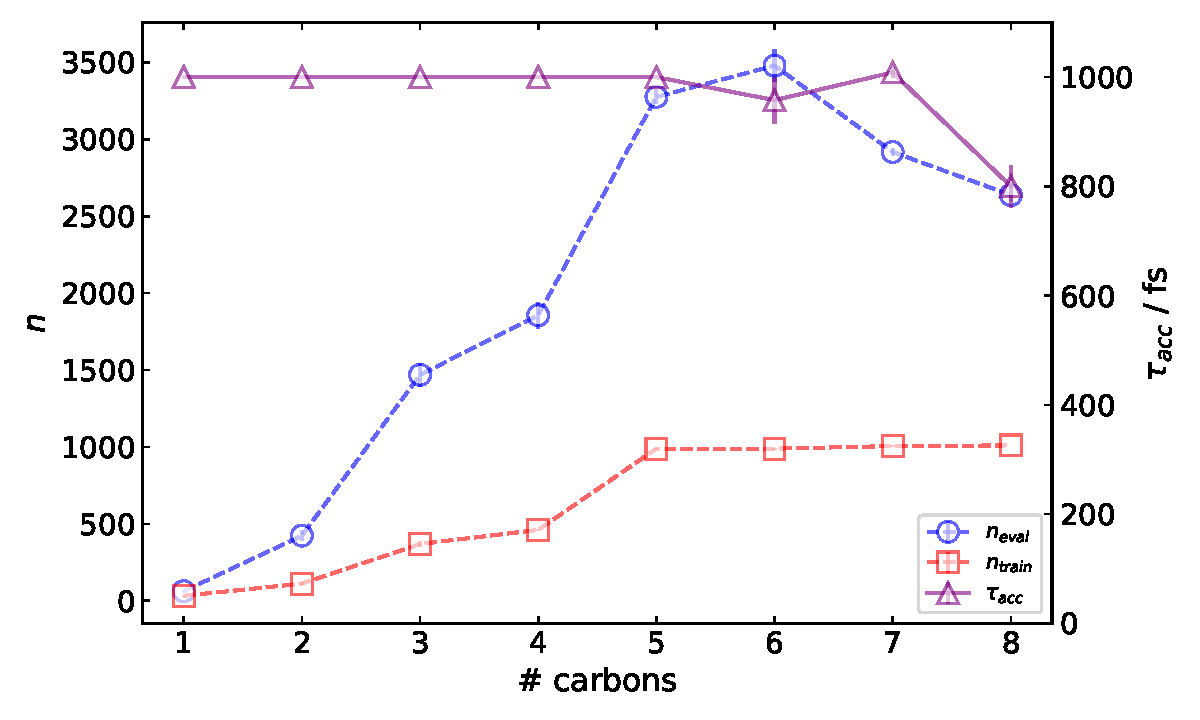
\includegraphics[height=6.5cm]{figSX3.pdf}
	\vspace{0.1cm}
	\hrule
	\vspace{0.1cm}
	\caption{Number of reference evaluations ($n_\text{eval}$) and number of training configurations ($n_\text{train}$) generated in 100 active learning loops for a linear alkane chain (500 K, 1 \kcal~ AL threshold, GFN2-XTB reference method). $\tau_\text{acc}$ is an average from three simulations, $E_l$ = 1 \kcal, $E_t = 10E_l$, $T = 300$ K, $\max(\tau_\text{acc}) = 1$ ps.}
	\label{fig::SX3}
\end{figure}


\subsection{Small Organic Molecules}


\comment{
	TJW:  Maybe not worth the faff for the SI, but can we have the numbers not overlapping? It makes 23(?) and 29(?) hard to see on the n_train graph.
	TJW: It's interesting that benzene is so low, while cyclohexane is fairly high, even though they are both quite symmetric (other than the different conformations cyclohexane can take.
	TJW: Can you mention a brief summary of what the complexity metric is and can you also mention in the S3 caption you have scaled the values by this complexity metric?
}


A selection of solvents and small organic molecules (\figurename{ \ref{fig::SX4}}, inc. $>2$ elements) forms a diverse set over which system scaling can be more realistically determined. 

Unlike the alkanes, there is no obvious trend in the number of evaluations required to train a chemically accurate potential. Even correlating against a general complexity metric\cite{Bertz1981} reveals little to no correlation aside from a general increase.

\begin{figure}[h!]
	\centering
	\vspace{0.4cm}
	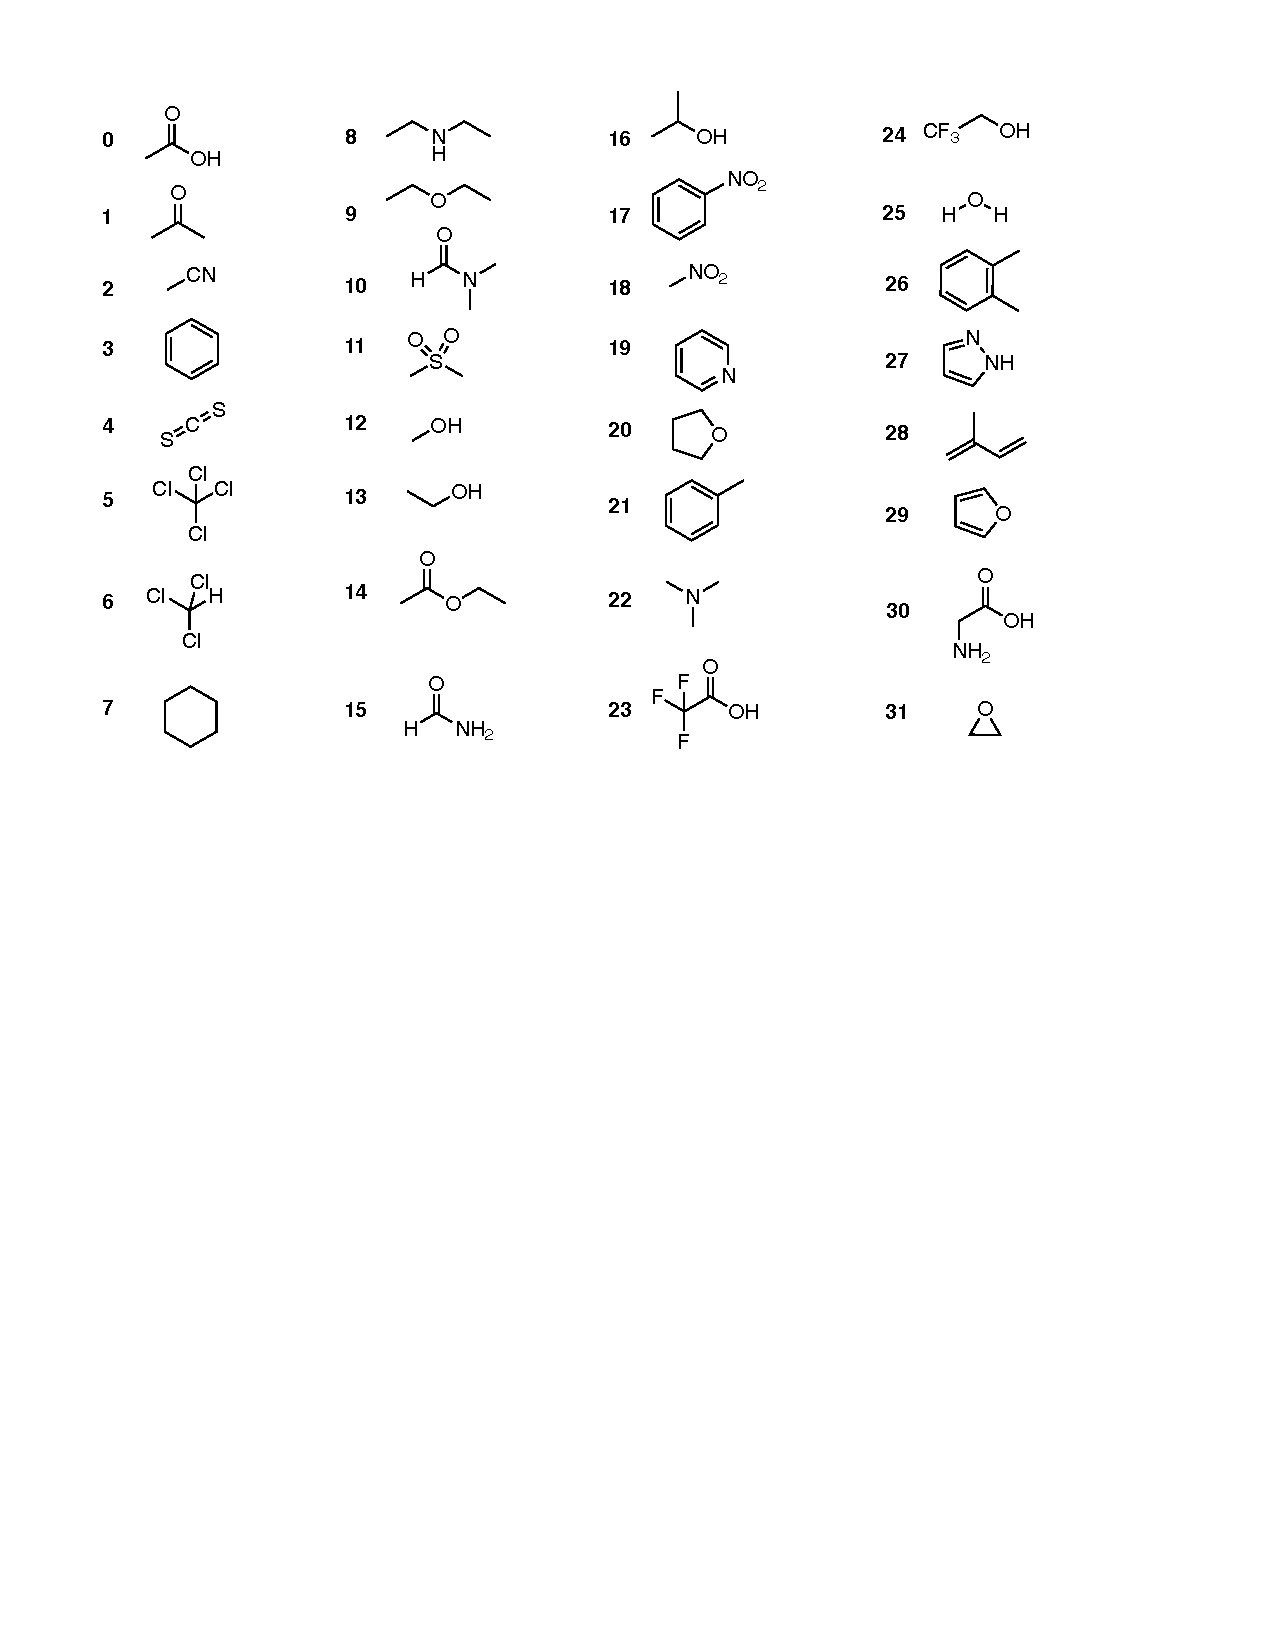
\includegraphics[width=0.9\textwidth]{figSX4.pdf}
	\vspace{0.2cm}
	\hrule
	\vspace{0.1cm}
	\caption{Small molecules used in \figurename{ \ref{fig::SX5}}.}
	\label{fig::SX4}
\end{figure}


\begin{figure}[h!]
	\centering
	\vspace{0.4cm}
	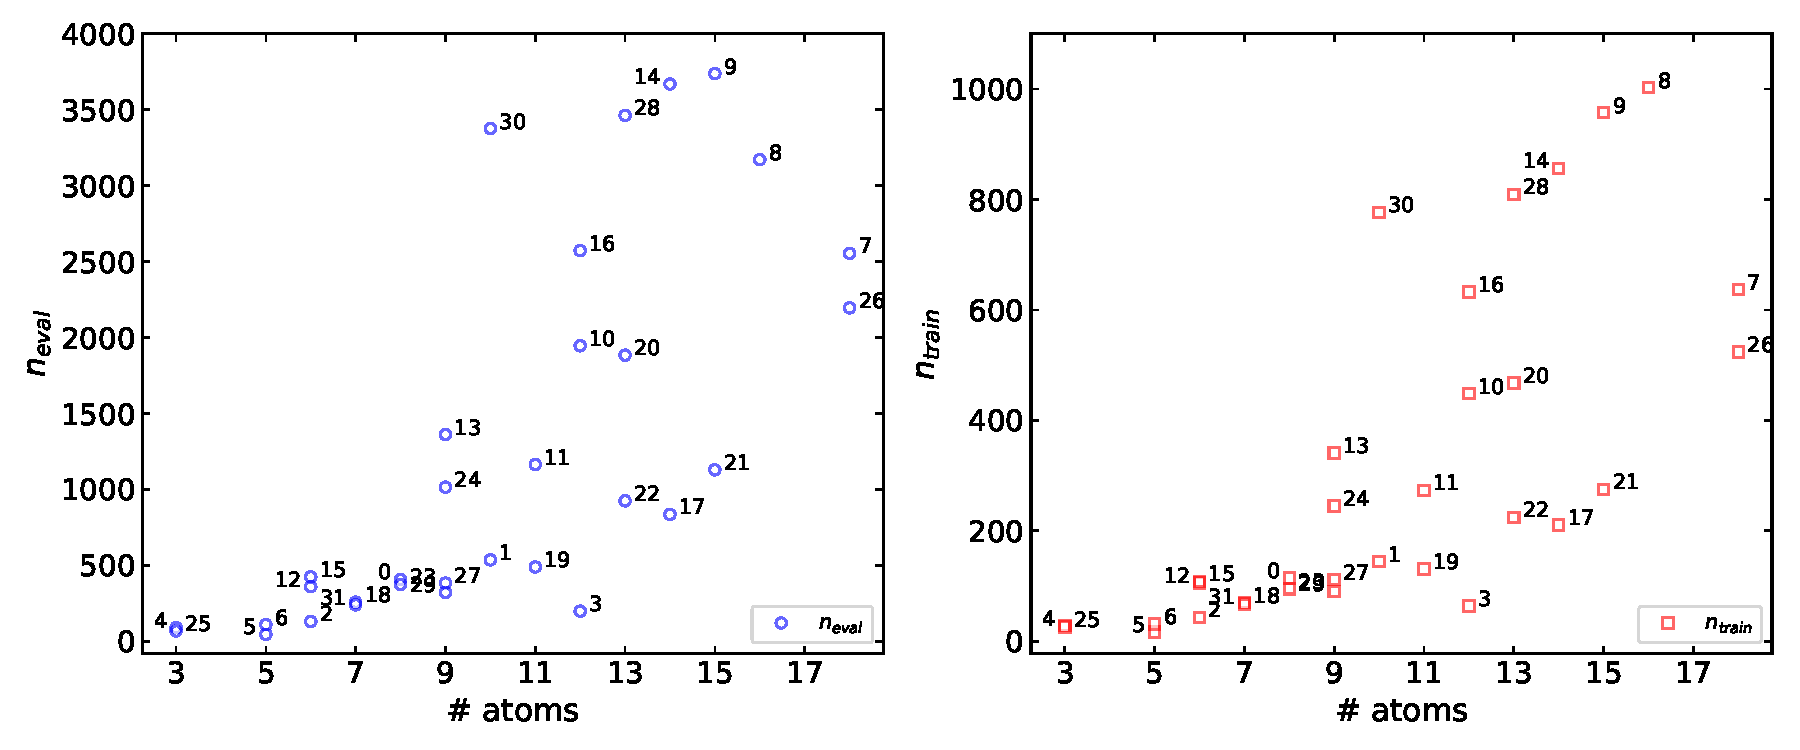
\includegraphics[width=\textwidth]{figSX5.pdf}
	\hrule
	\vspace{0.1cm}
	\caption{Number of reference evaluations ($n_\text{eval}$) and number of training configurations ($n_\text{train}$) required to generate a GAP with \tacc $>1$ ps (parameters as \figurename{ \ref{fig::SX3}}) for a variety of small molecules. Values (averages) and standard errors of the mean are taken over three training repeats with different initial random displacements.}
	\label{fig::SX5}
\end{figure}



\clearpage
\section{Hyperparameter Optimisation} \label{section::SI_hyperparam_opt}
\label{section::hyperparam_opt}

\subsection{QM Convergence}


Using ORCA v. 4.2.1 the default SCF and DFT integration grids provide essentially converged forces (\figurename{ \ref{fig::SX1}}) thus the defaults are used throughout. The error introduced is negligible compared to the `expected error' in the forces used in the GAP fitting ($\sigma_F = 0.1$ eV \AA~by default), thus default ORCA parameters will be used herein.


\begin{figure}[h!]
	\centering
	\vspace{0.4cm}
	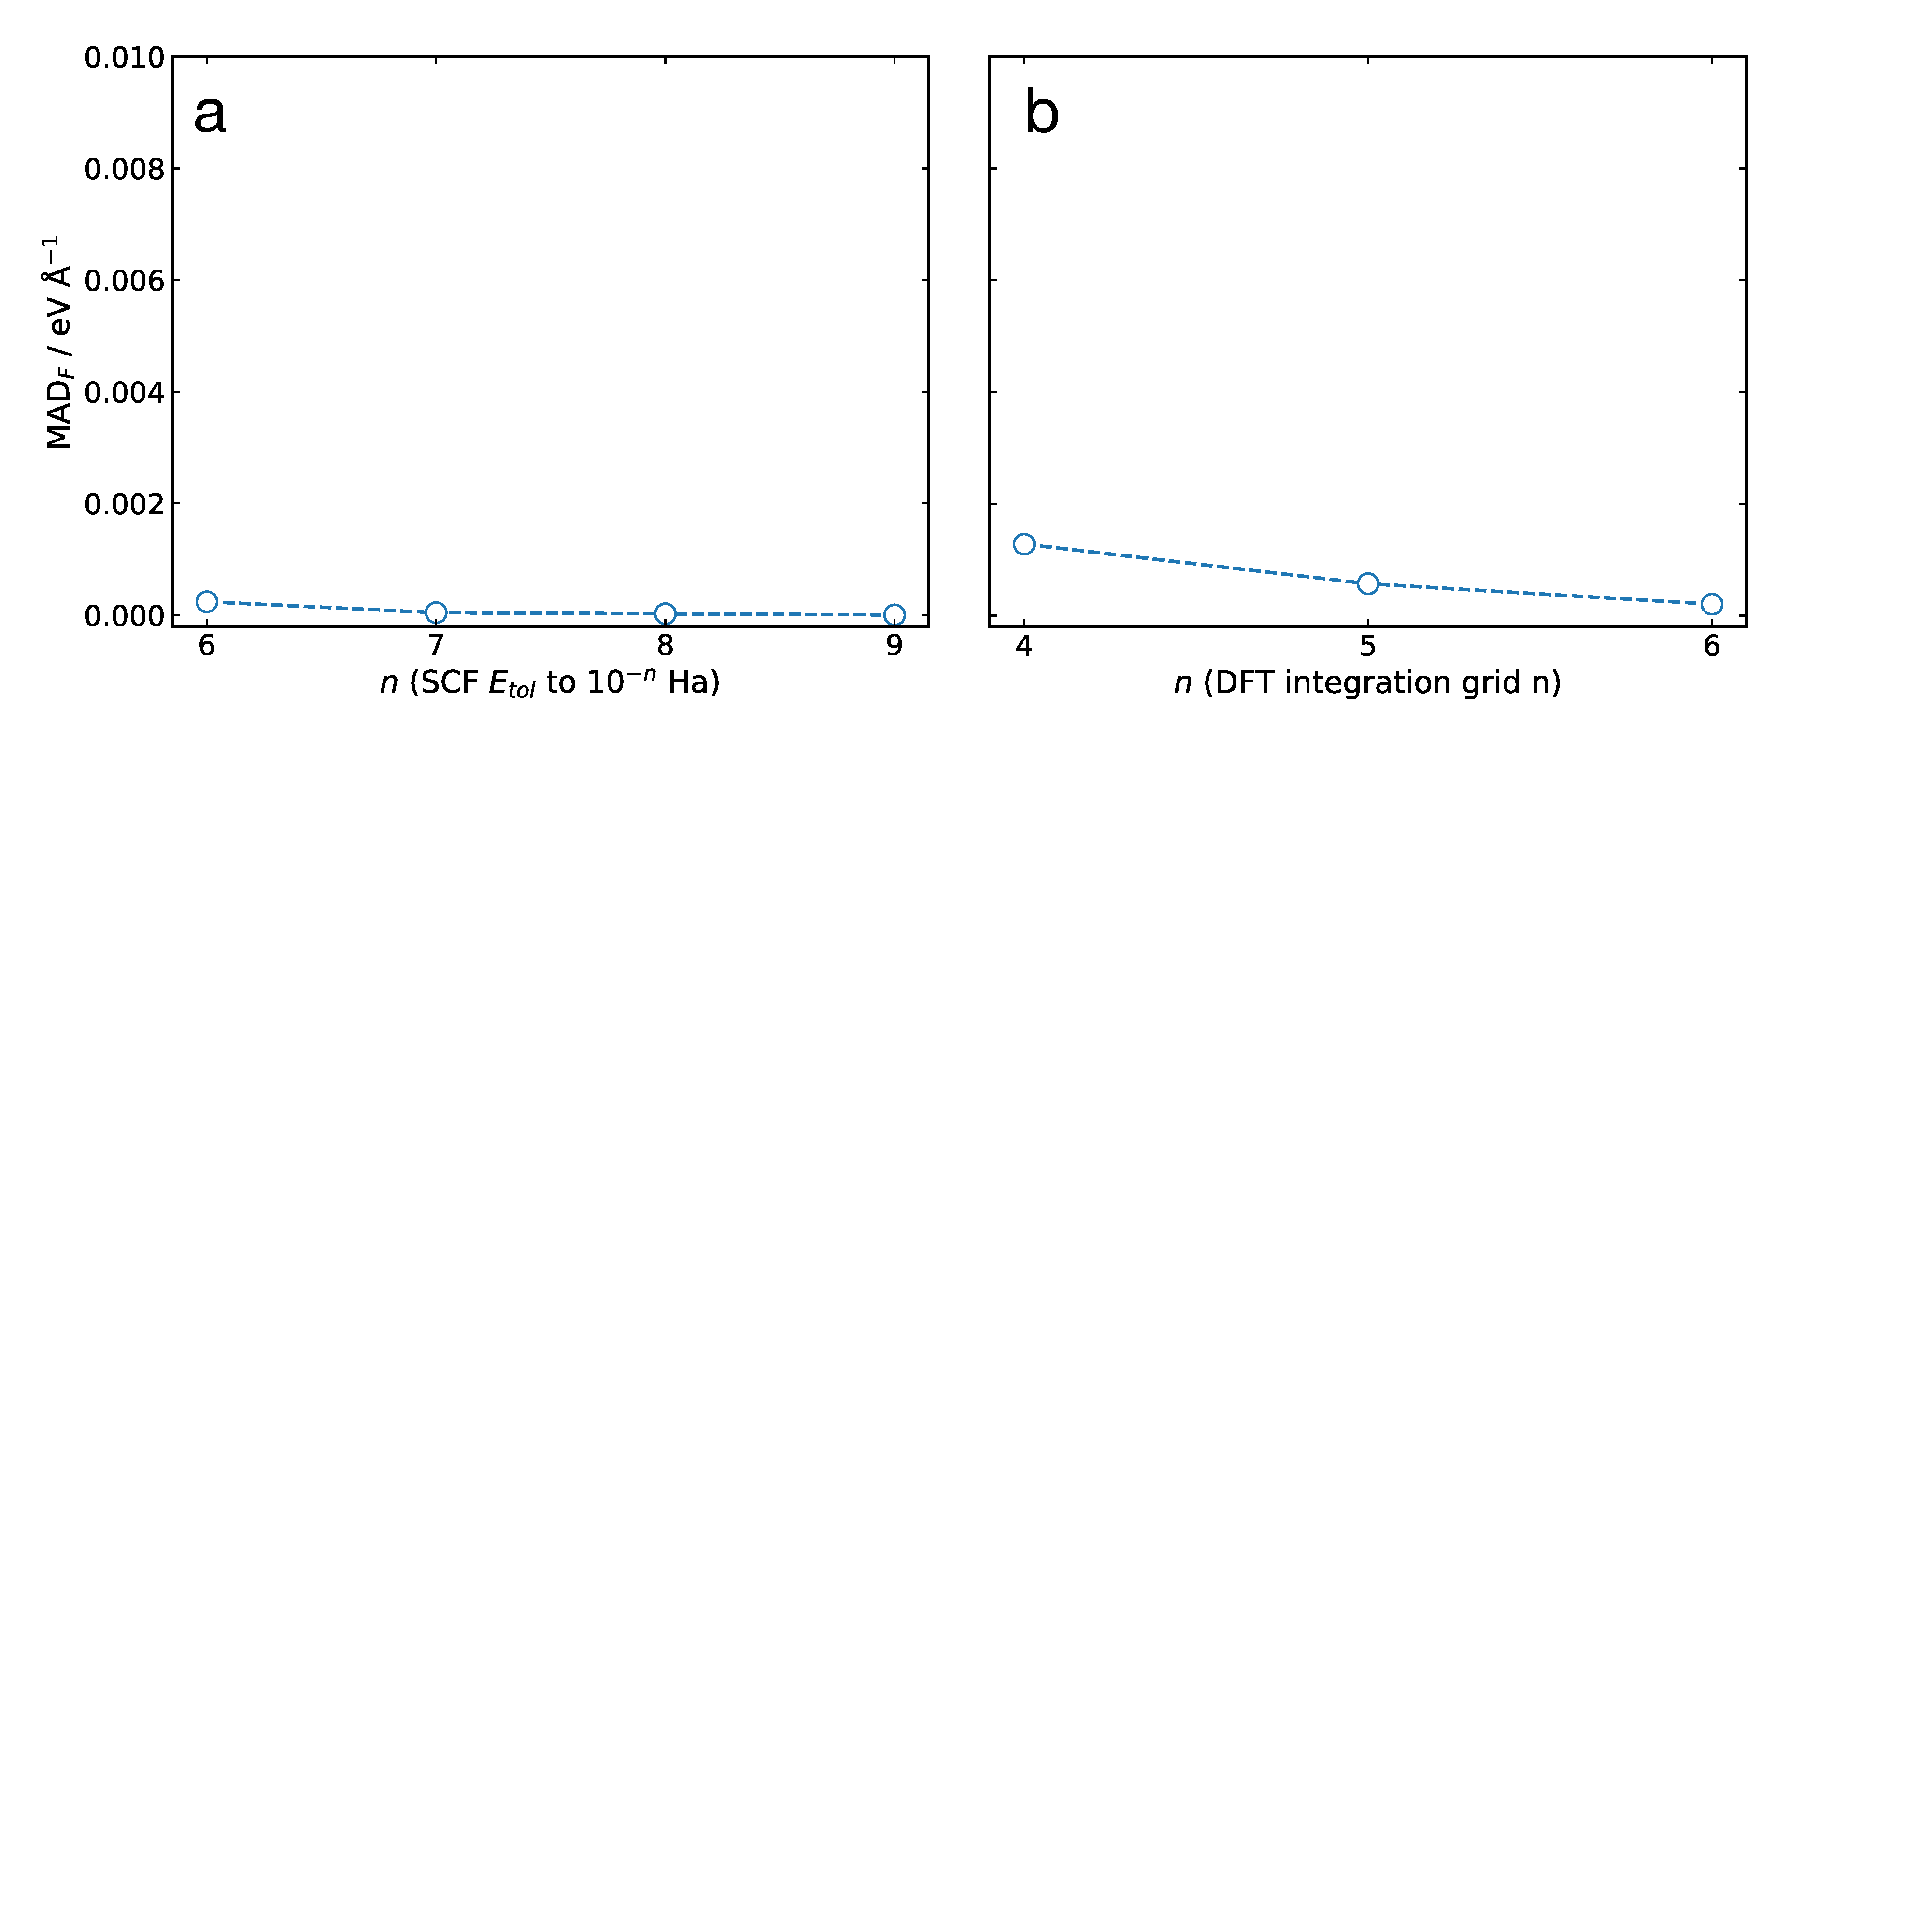
\includegraphics[height=6.4cm]{figSX1.pdf}
	\vspace{0.1cm}
	\hrule
	\vspace{0.1cm}
	\caption{Convergence of the force components of 10 randomly selected frames from an active learning instance from the TS of ethene+butadiene at the PBE/def2-SVP level of theory in ORCA. Convergence of the mean absolute deviation in forcers for the SCF energy change ($E_\text{tol}$) convergence (a) and DFT integration grid (b) is with respect to their maximum values in ORCA ($10^{-10}$ Ha and 7 respectively). The maximum MAD is 10$\times$ less than the default GAP $\sigma_F$.}
	\label{fig::SX1}
\end{figure}


\subsection{Expansion Order}

Increasing the expansion order of the SOAP provides an improved approximation to the overlap between two atomic densities in the (dot product SOAP) kernel. Therefore, the energies and forces should be converged with respect to $n_\text{max}$ and $l_\text{max}$, being aware of the increased computational cost of the SOAP computation. A slightly larger order of 8 in both $l_\text{max}$ and $n_\text{max}$  provides the optimum value, requiring a third of the training data to achieve a chemically accurate potential for propane (\figurename{ \ref{fig::SX2}}). Similar results are obtained for pentane over a smaller $n_\text{max}$, $l_\text{max}$ window, albeit without the exponential decay observed in \figurename{ \ref{fig::SX2}}. As found in other works (e.g. ref. \cite{Rowe2020}), accuracy converges faster with respect to $l_\text{max}$ than $n_\text{max}$ (\figurename{ \ref{fig::SX6}}b). Interestingly, decreasing the radial expansion order seems to reduce inhibit training slightly ($n_\text{max} = l_\text{max} = 8$ in \figurename{ \ref{fig::SX6}a} cf.$n_\text{max} = 8, l_\text{max} = 4$ in \figurename{ \ref{fig::SX6}b} ).


\comment{
	TJW:  10x1 ps GAP-MD?
	TJW: Why is the graph for propane convex while pentane is concave?
}


\begin{figure}[h!]
	\centering
	\vspace{0.4cm}
	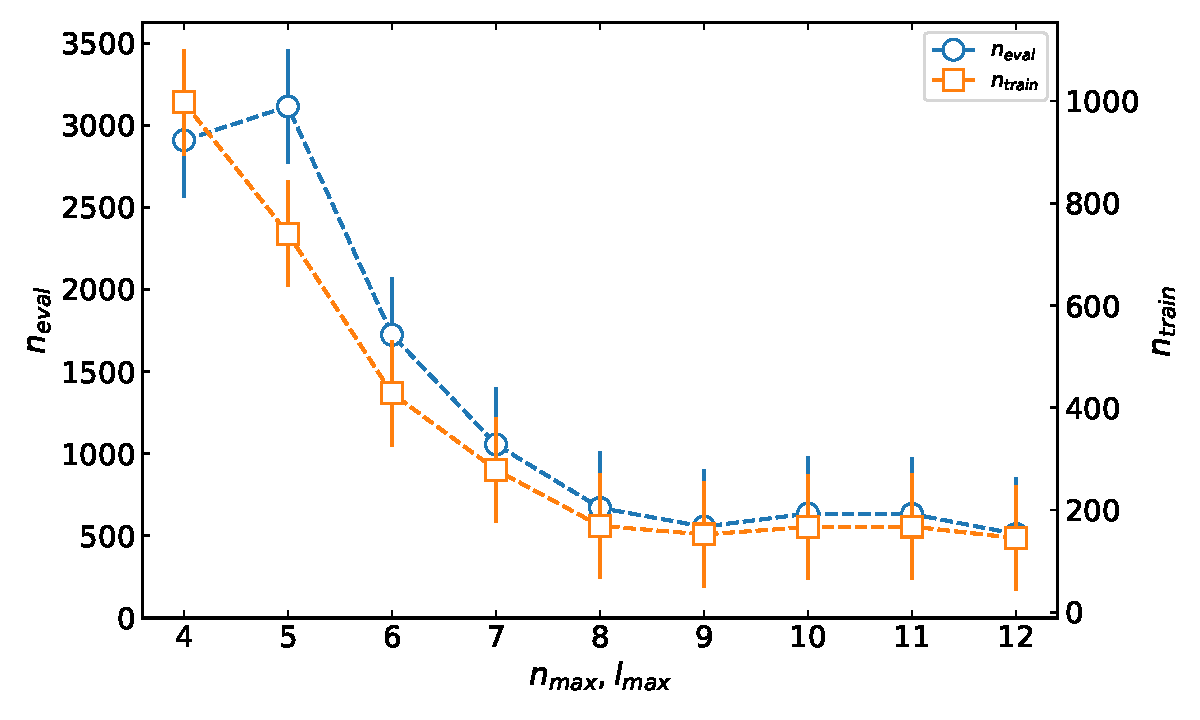
\includegraphics[height=6.4cm]{figSX2.pdf}
	\vspace{0.0cm}
	\hrule
	\vspace{0.1cm}
	\caption{Number of reference evaluations ($n_\text{eval}$) and number of training configurations ($n_\text{train}$) required to propagate 10, 1 ps  GAP-MD at 500 K without finding a prediction with an error $> 1$ \kcal~from the true GFN2-XTB reference at a particular order of radial and angular SOAP expansion ($n_\text{max},\, l_\text{max}$) for propane. Other hyperparameters as \tablename{ \ref{table::default_params}}.}
	\label{fig::SX2}
\end{figure}


\begin{figure}[h!]
	\centering
	\vspace{0.4cm}
	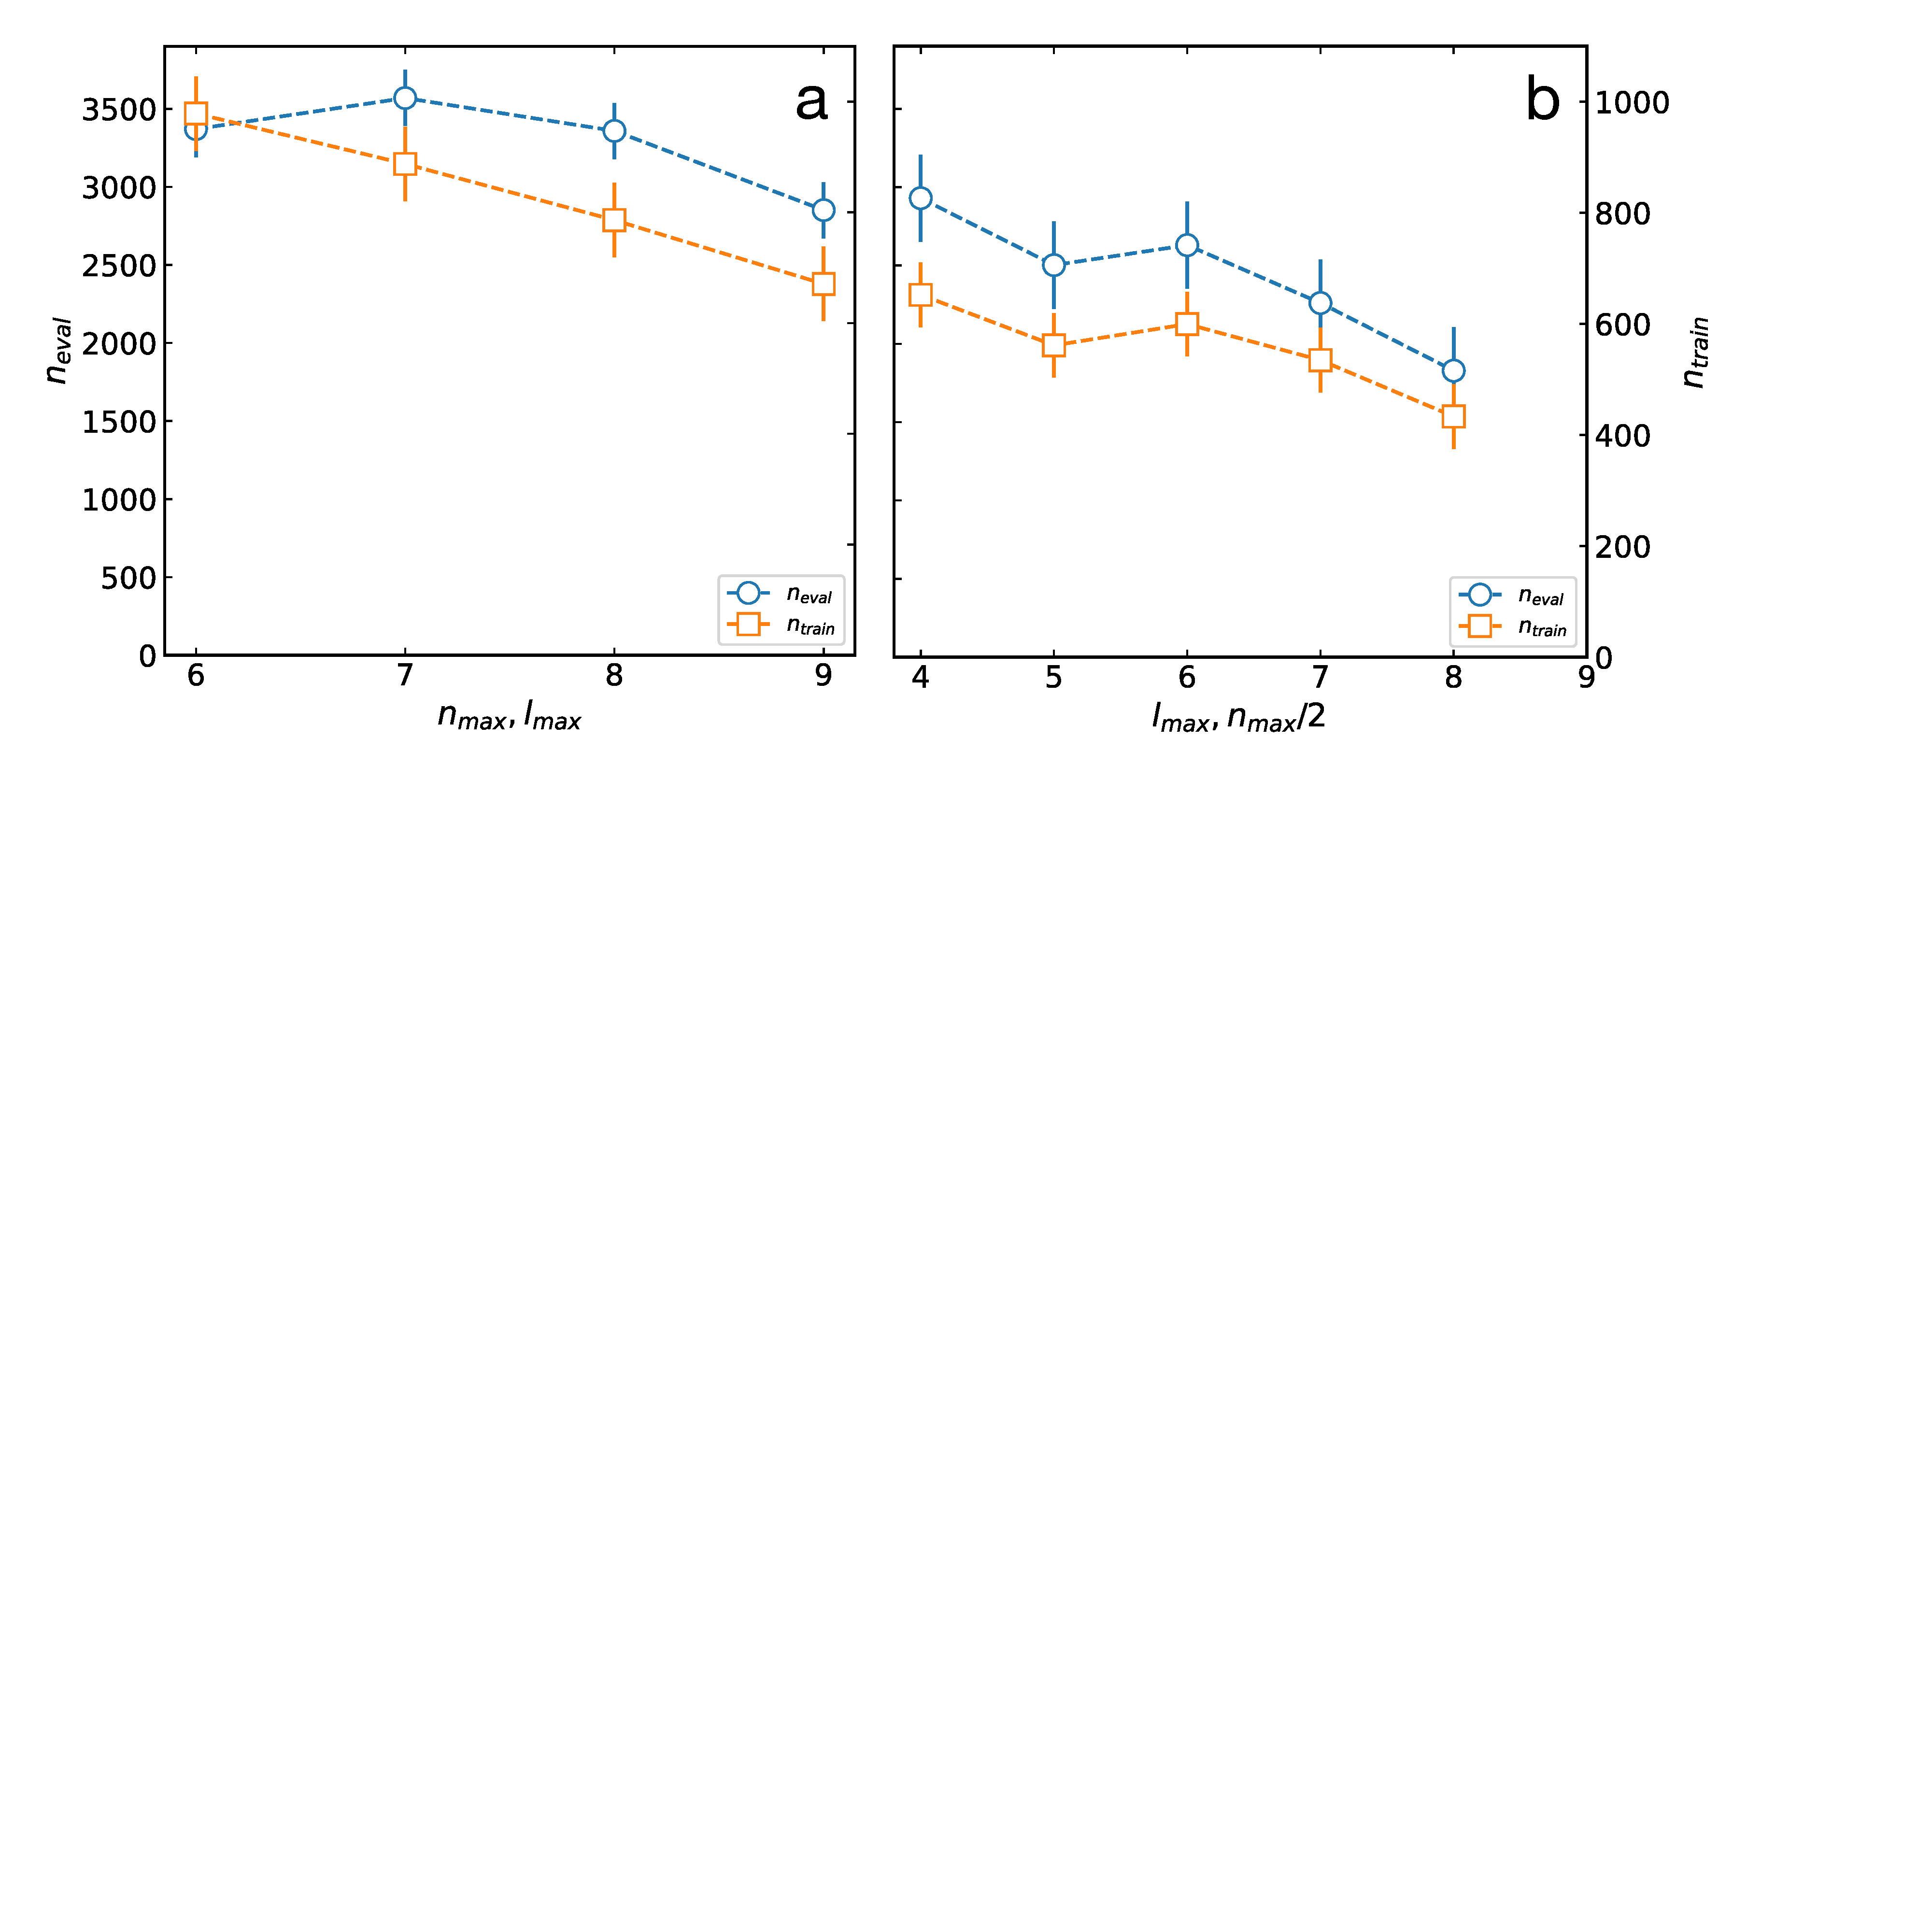
\includegraphics[height=6.4cm]{figSX6.pdf}
	\vspace{0.2cm}
	\hrule
	\vspace{0.1cm}
	\caption{As \figurename{ \ref{fig::SX2}} for pentane with (a) $n_\text{max} = l_\text{max}$ and (b) $n_\text{max} = 2l_\text{max}$ .}
	\label{fig::SX6}
\end{figure}


\clearpage
\subsection{Expected Errors}

\comment{
	TJW: What do you mean by expected errors?
}

Using $n_\text{max} = l_\text{max} = 8$ and optimising the `expected errors' in the energy and forces in training a gas-phase GAP for propane, increasing the `smoothness' (larger $\sigma_E$) is not beneficial to the active learning rate (\figurename{ \ref{fig::SX7}}). Instead, fitting energies and forces more \emph{strongly} (top right, \figurename{ \ref{fig::SX7}}) enables only 75 training configurations required for an accurate propane potential.\footnote{Note that visualisation of a short 1 ps MD trajectory at 500 K suggests the potential is reasonable and is not circumventing the \tacc error metric.} Repeating the same along a slice in the ($\sigma_E$,  $\sigma_F$) space suggests that this result it not limited to just small systems (\figurename{ \ref{fig::SX9}}), no the choice of expansion order.


\begin{figure}[h!]
	\centering
	\vspace{0.4cm}
	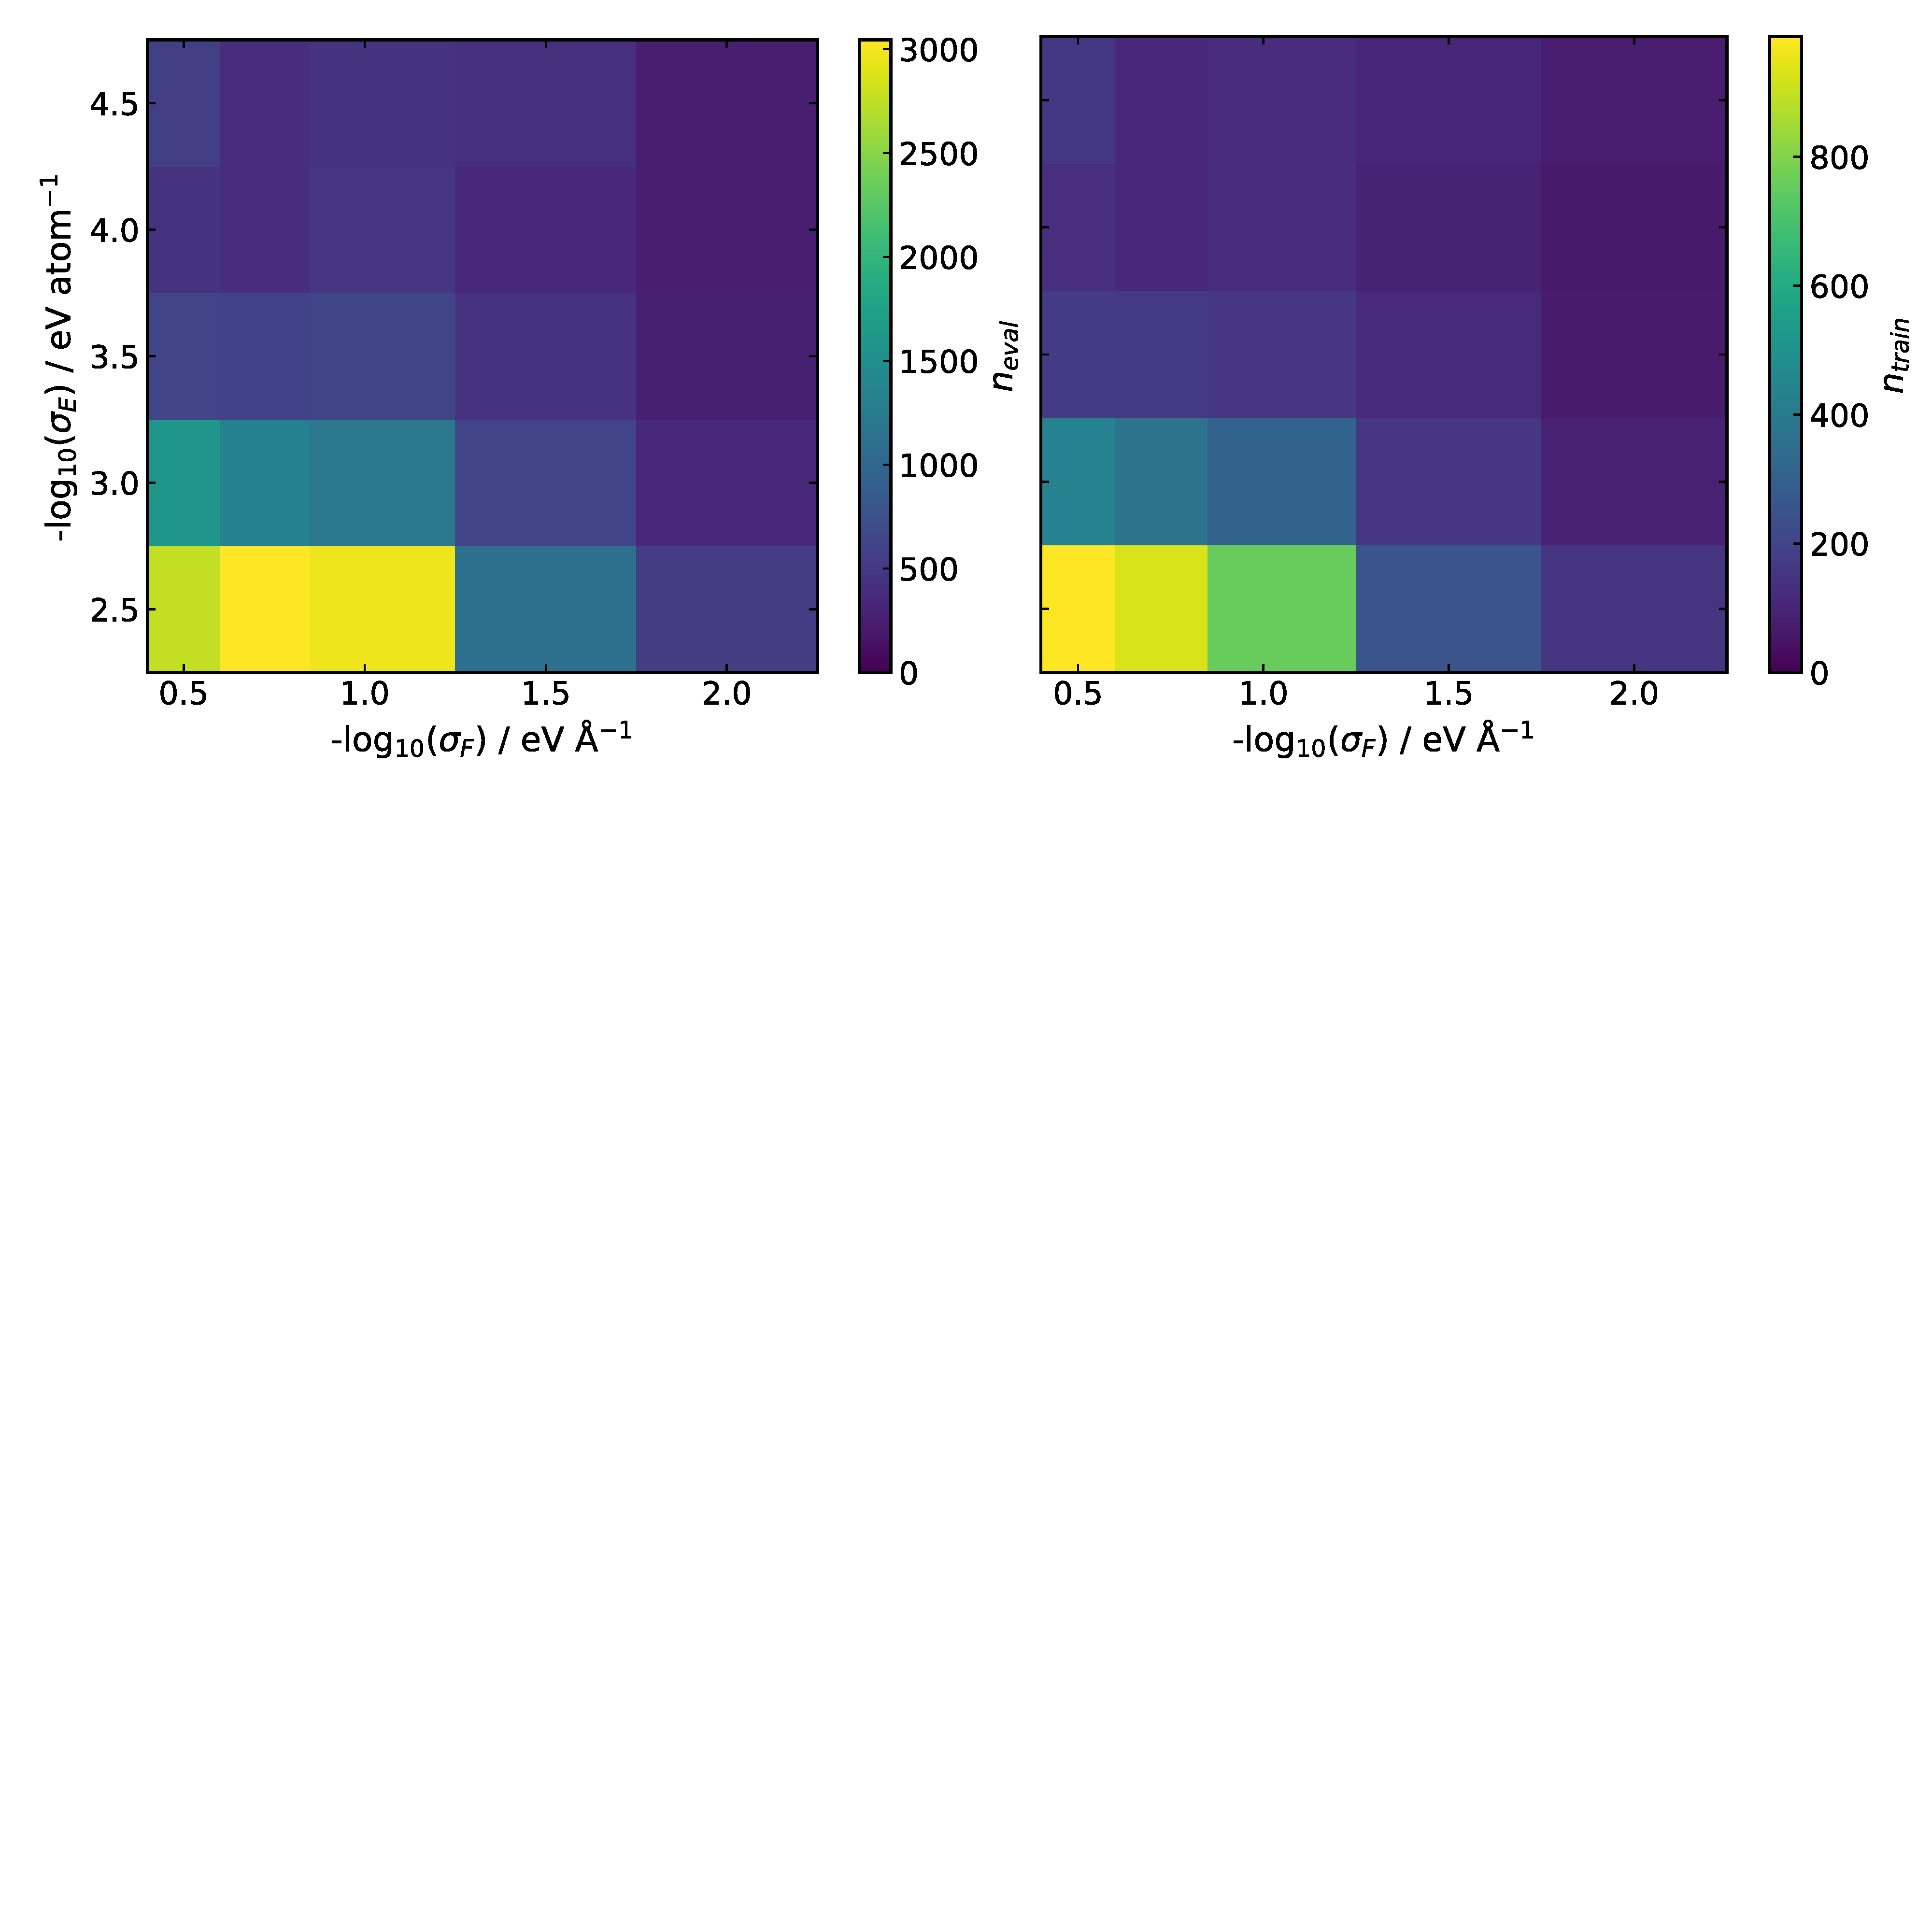
\includegraphics[height=6.4cm]{figSX7.pdf}
	\vspace{0.2cm}
	\hrule
	\vspace{0.1cm}
	\caption{Number of evaluations required to generate a chemically accurate GAP (as \figurename{ \ref{fig::SX2}}) for propane as a function of $\sigma_E$ and $\sigma_F$. Values are averages over three independent repeats.}
	\label{fig::SX7}
\end{figure}


\begin{figure}[h!]
	\centering
	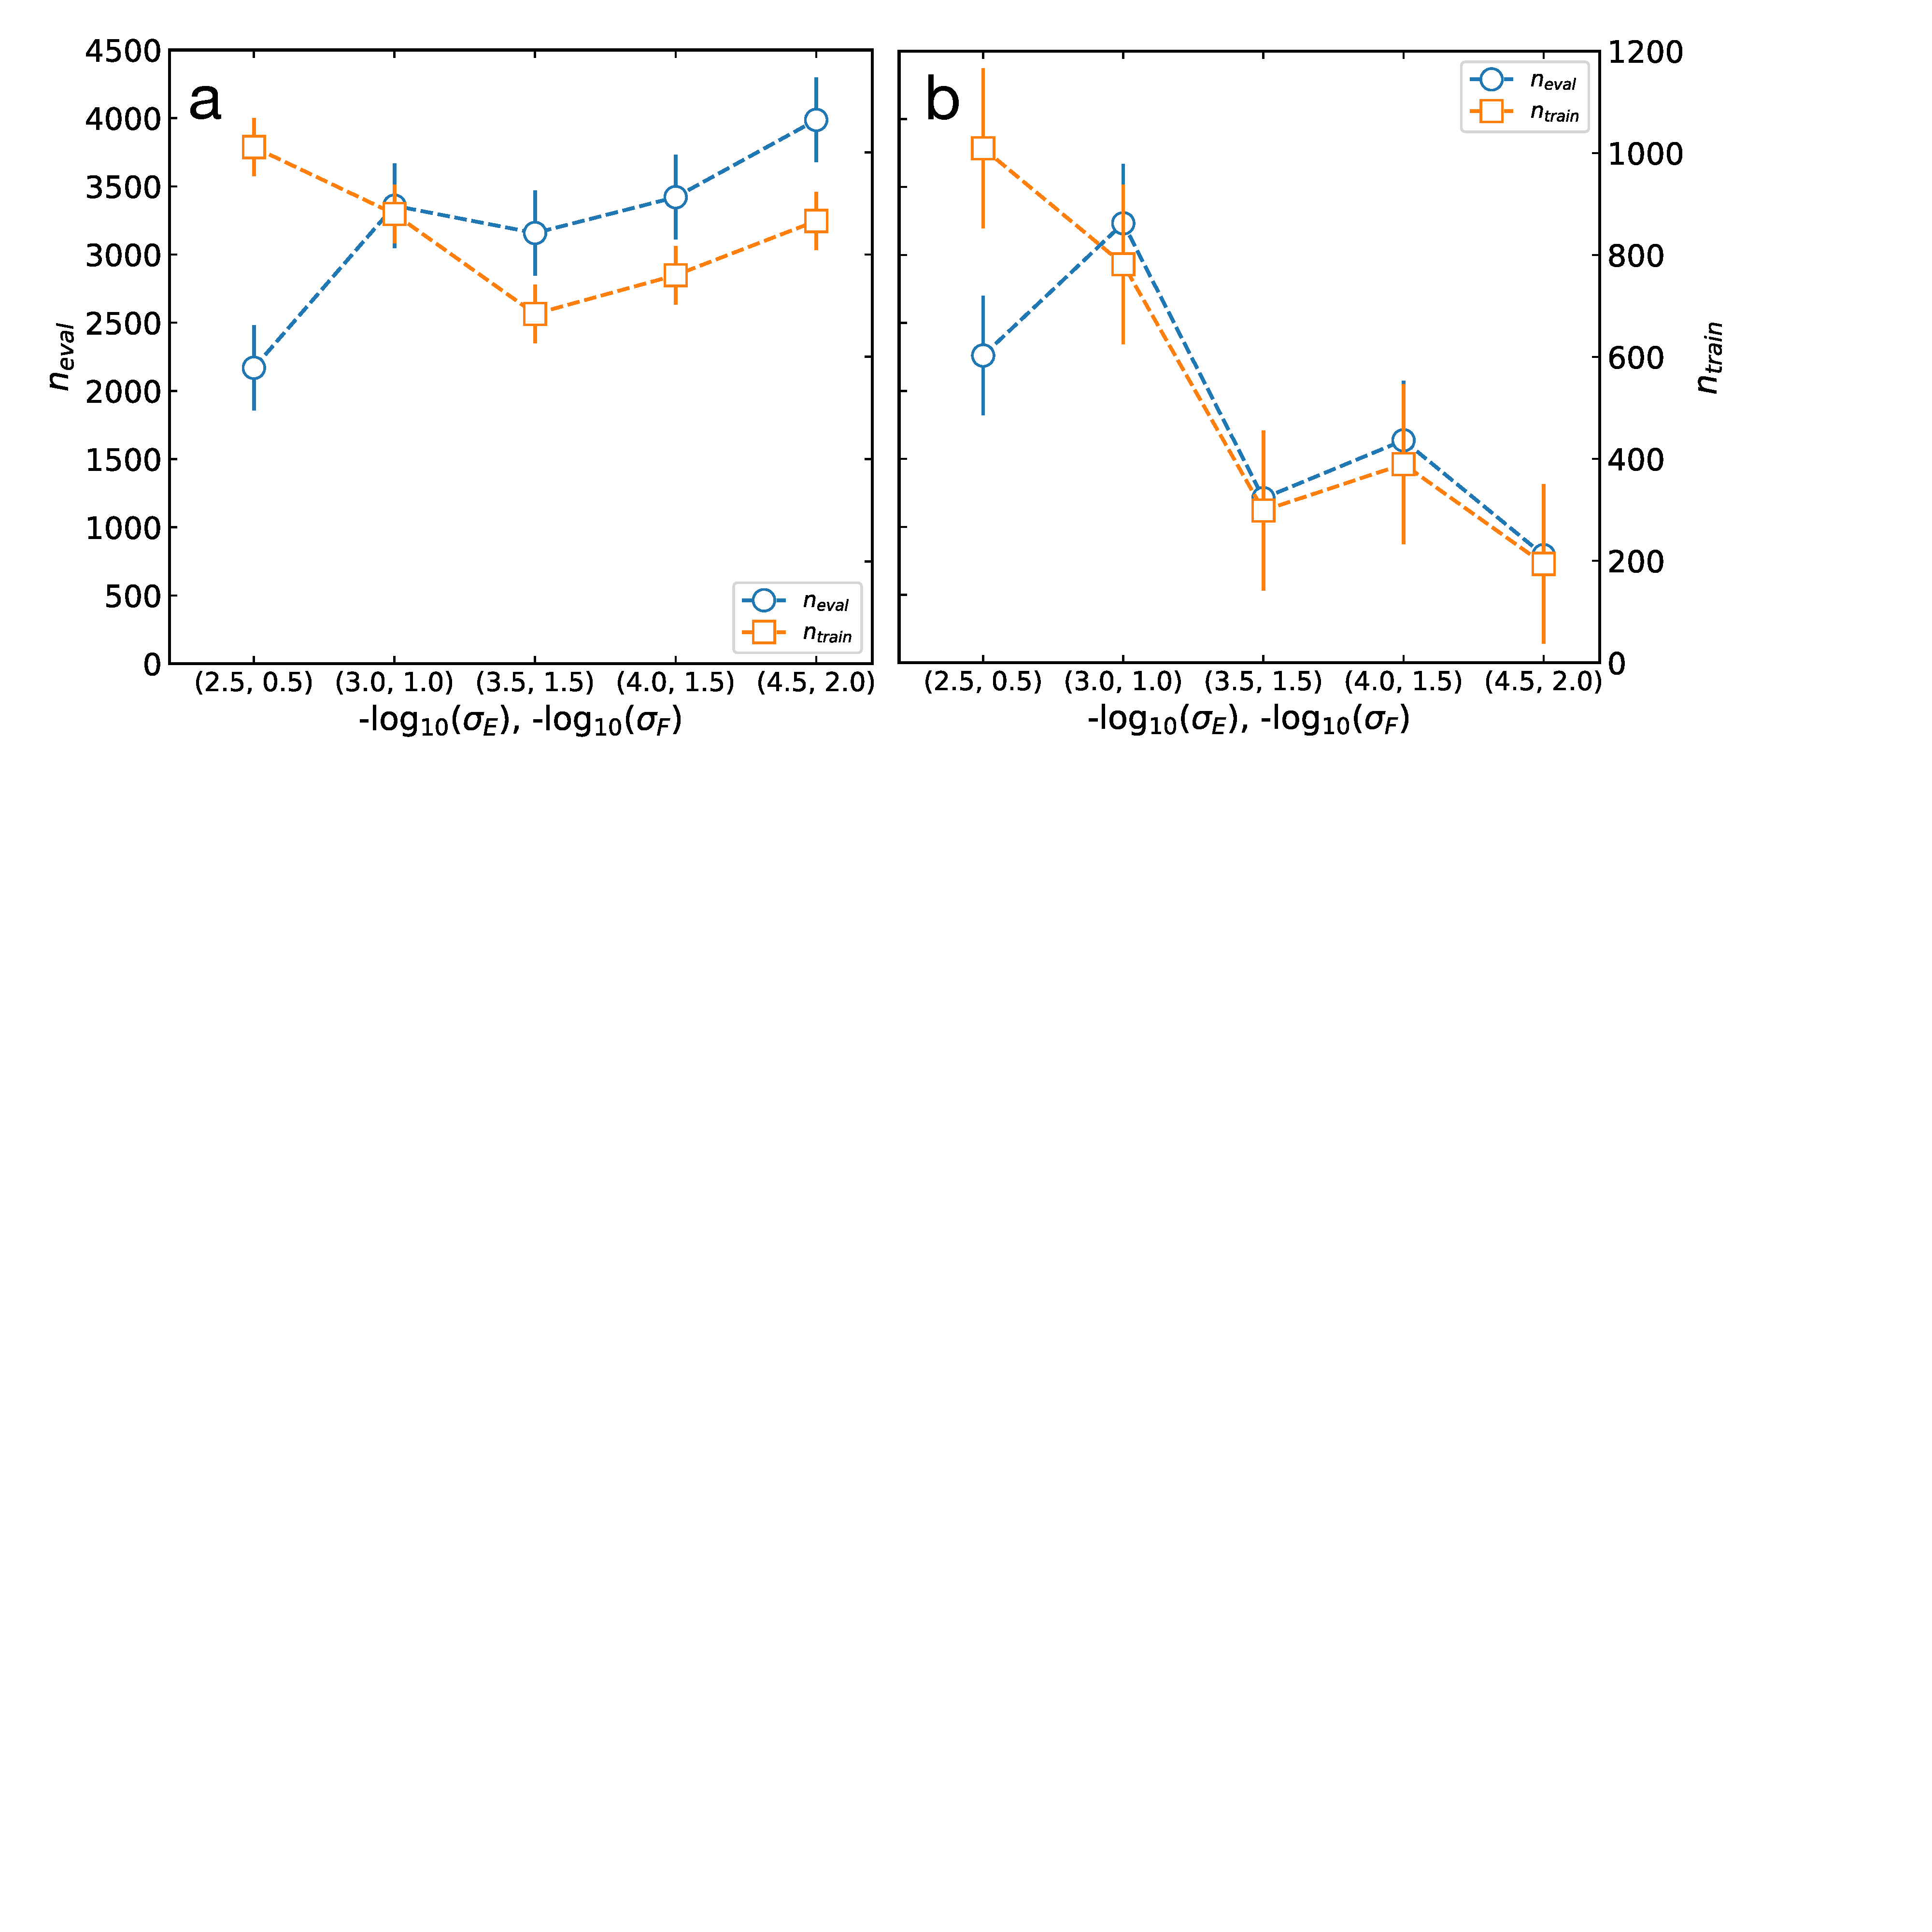
\includegraphics[height=6.4cm]{figSX9.pdf}
	\vspace{0.1cm}
	\hrule
	\vspace{0.1cm}
	\caption{As \figurename{ \ref{fig::SX7}} for pentane along a slice of the 2D space with (a) $n_\text{max} = l_\text{max} = 8$, (b) $n_\text{max} = 12, l_\text{max} = 6$.}
	\label{fig::SX9}
\end{figure}

Here, it is important to emphasize that the pentane potential trained using 500 K active learning at the GFN2-XTB level with the \emph{strongest} fitting ($\sigma_E = 10^{-4}$ eV atom${}^{-1}$, $\sigma_F = 10^{-2}$ eV \AA$^{-1}$, bottom right \figurename{ \ref{fig::SX9}}) is highly accurate over 'long-time' dynamics (\figurename{ \ref{fig::SX20}}).


\begin{figure}[h!]
	\centering
	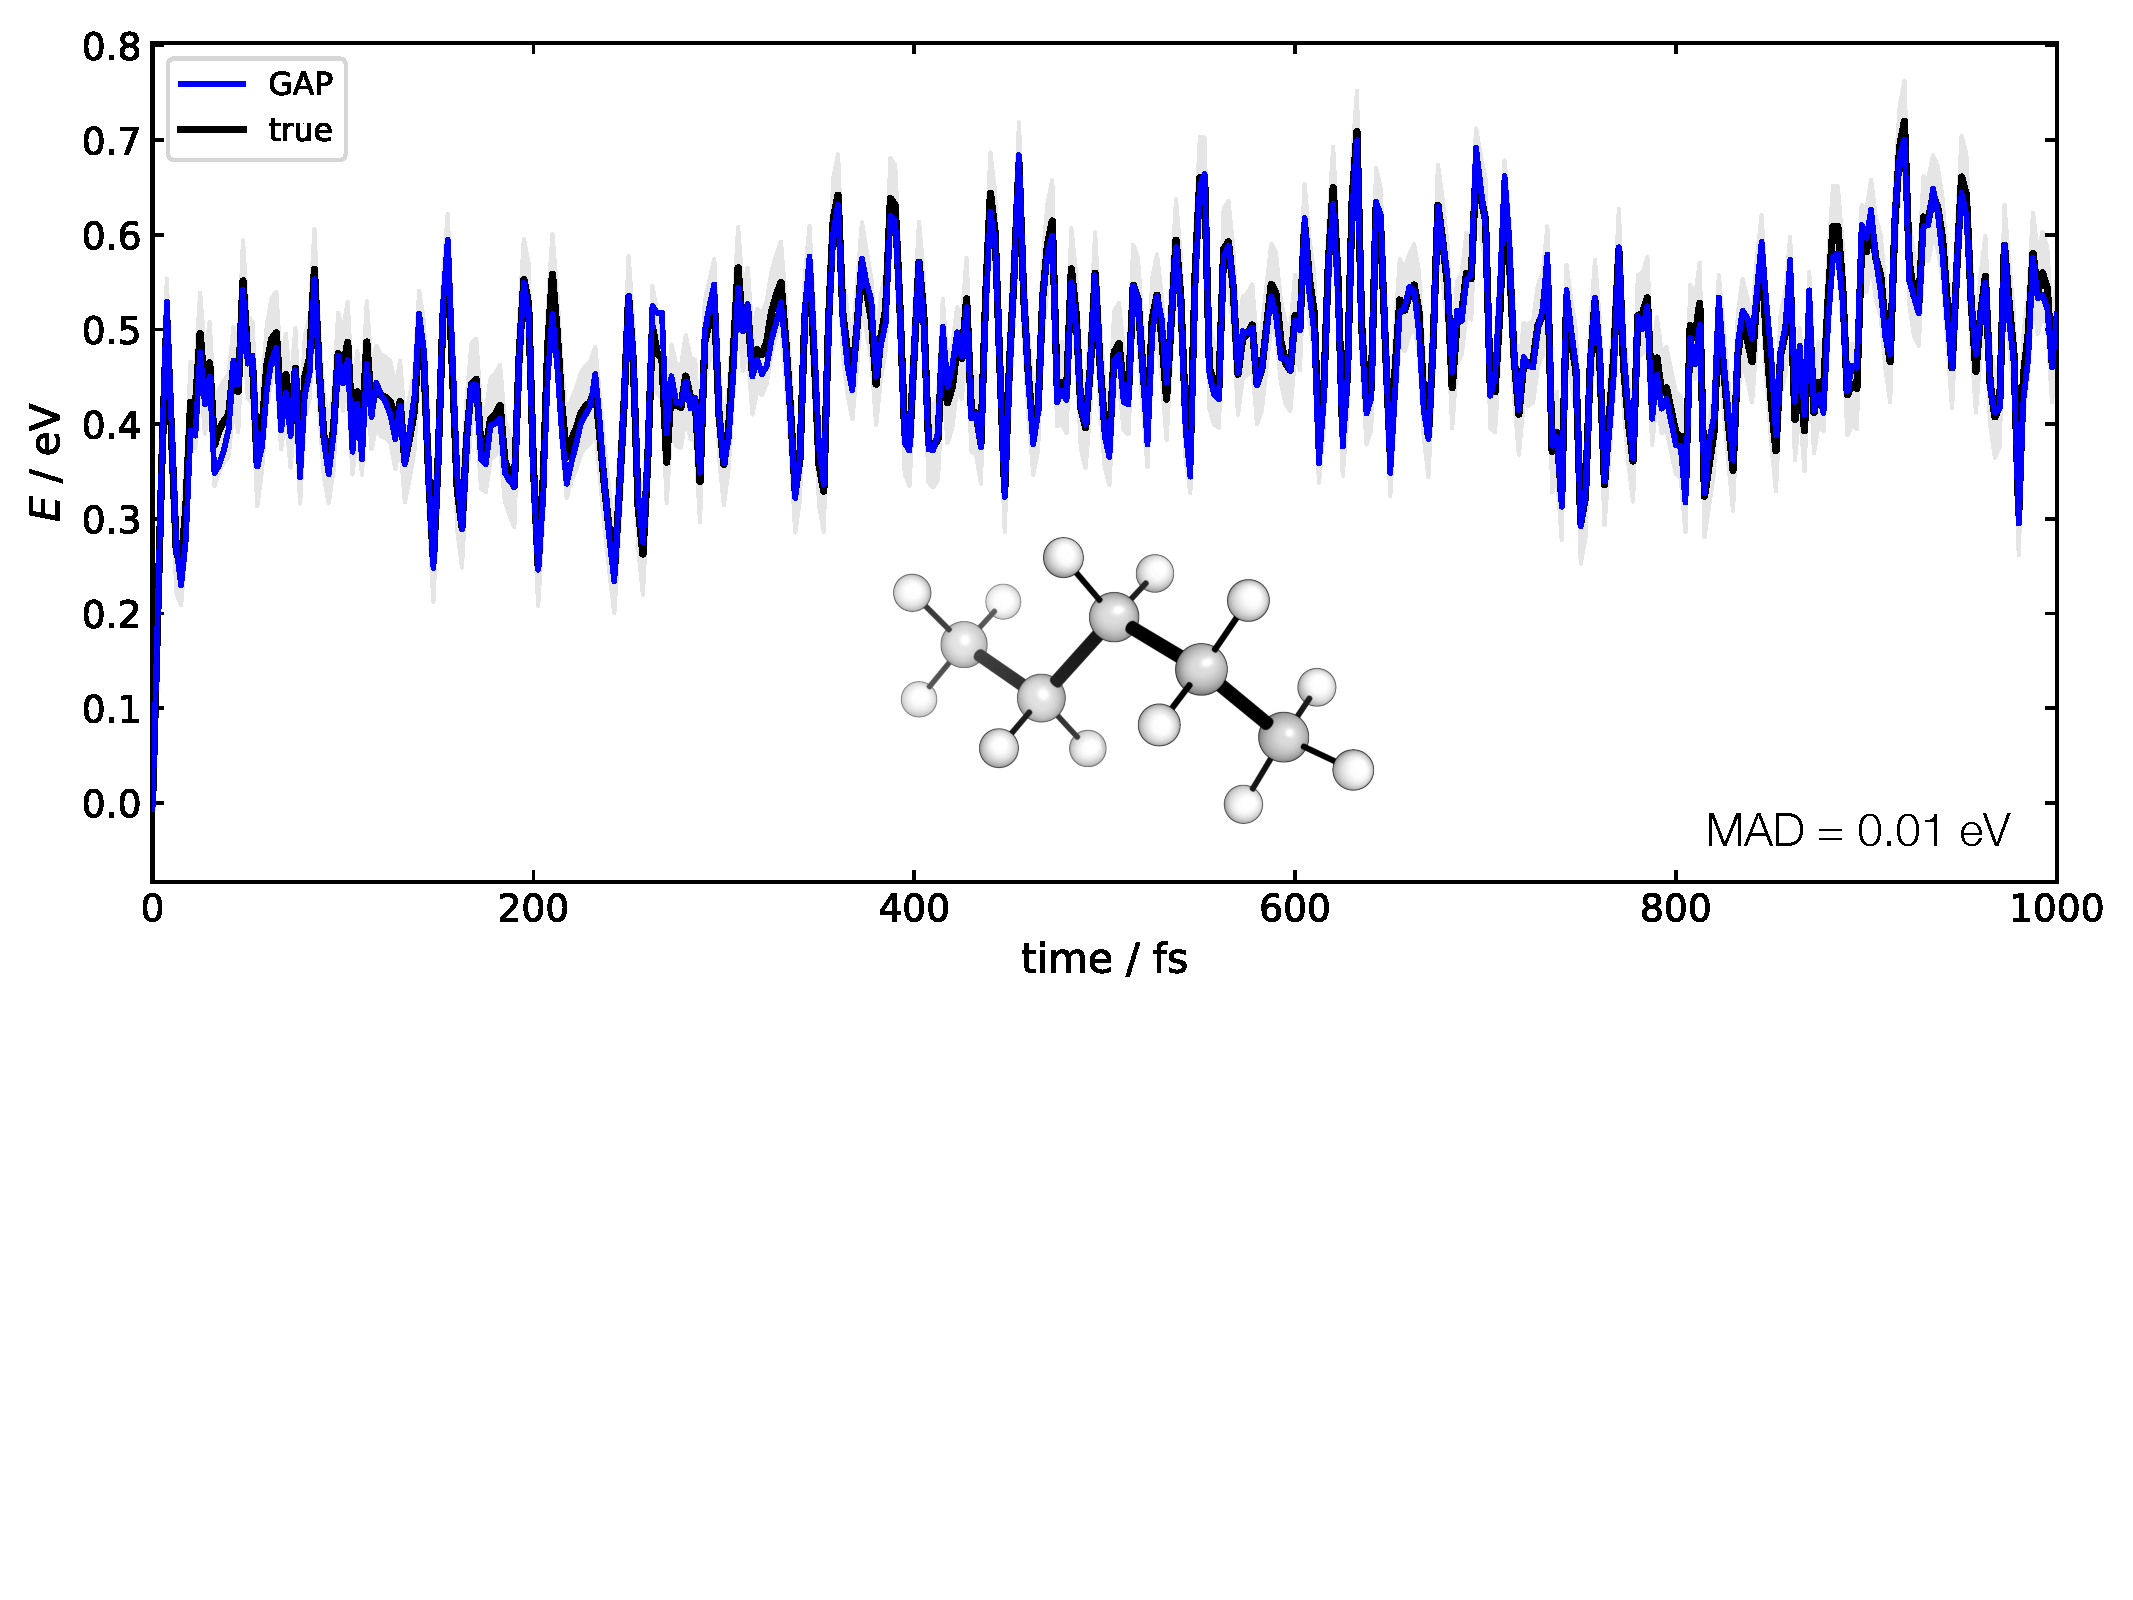
\includegraphics[height=6.4cm]{figSX20.pdf}
	\vspace{0.1cm}
	\hrule
	\vspace{0.1cm}
	\caption{GAP-MD dynamics at 300 K (dt = 0.5 fs, 50 \AA~cubic box equivalent to a vacuum) compared to GFN2-XTB ground truth. $\sigma_E = 10^{-4}$ eV atom${}^{-1}$, $\sigma_F = 10^{-2}$ eV \AA$^{-1}$, 500 K active learning.}
	\label{fig::SX20}
\end{figure}


\newpage
\subsection{Sparse Points}

Previous studies have shown that GAP accuracy can converge exponentially with the number of atomic environments (`sparse points').\cite{Rowe2020}. Of course this will be system dependent, thus the scaling is evaluated for alkanes with 3, 4 and 5 carbons (\figurename{ \ref{fig::SX21}}). For these systems all GAPs are converged with respect to $n_\text{sparse}$ at 800 points. For pentane a substantial drop in the number of required evaluations is observed after 400 configurations, suggesting for `large' systems ($>15$ atoms) $n_\text{sparse}$ closer to 1000 is more suitable.


\begin{figure}[h!]
	\centering
	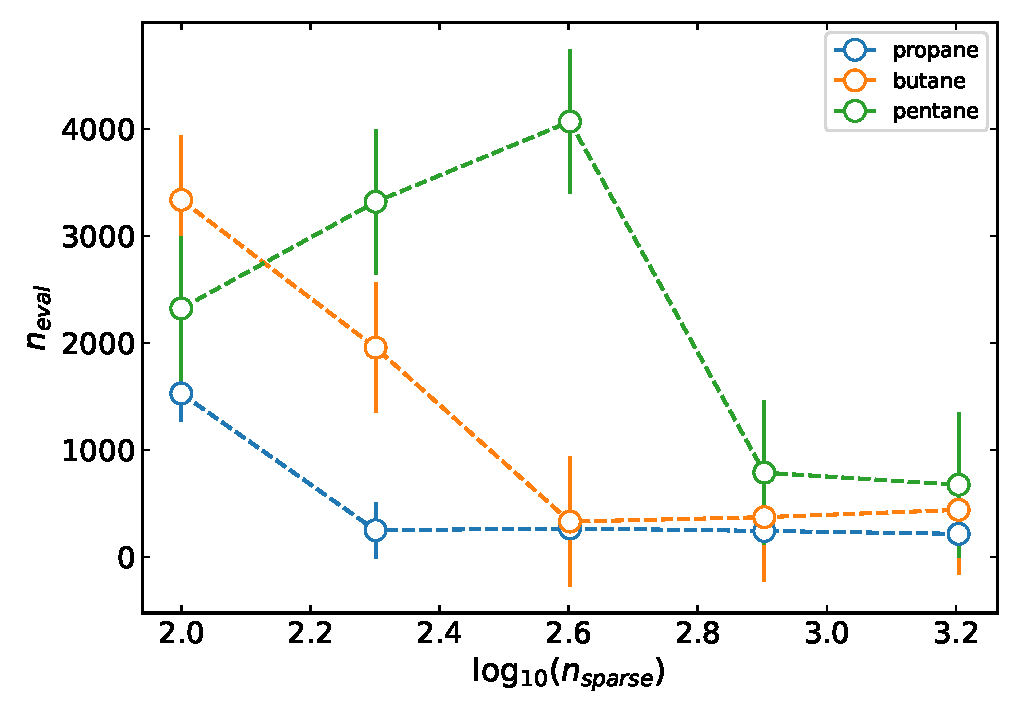
\includegraphics[height=6.4cm]{figSX21.pdf}
	\vspace{0.1cm}
	\hrule
	\vspace{0.1cm}
	\caption{Convergence of the number of evaluations required to generate a potential as \figurename{ \ref{fig::SX2}} for linear alkanes as a function of the sparse points. Error bars are standard errors of the mean over three independent repeats.}
	\label{fig::SX21}
\end{figure}


\subsection{Summary}

Based on these data, we suggest using the updated hyperparameters shown in \tablename{ \ref{table::updated_params}} for small molecules in the gas phase.

\begin{table}[h!]
	\def\arraystretch{1.3}
	\begin{tabularx}{\textwidth}{YYY}
		\hline
		Type&	Parameter	&Value\\
		\hline
		GAP	   &  $\sigma_E$	&  	0.1 meV atom${}^{-1}$ \\
			   &  $\sigma_F$	&  	0.01 eV \AA${}^{-1}$
		\\
		SOAP descriptors  
		&$n_\text{max}/2,$ $l_\text{max}$&6  \\
		 
		&$n_\text{sparse}$ &1000              
	\end{tabularx}
	\hrule
	\vspace{0.1cm}
	\caption{Updated hyperparameters parameter set for GAPs and SOAP descriptors, all other hyperparameters as {\tablename{ \ref{table::default_params}}}.}
	\label{table::updated_params}
\end{table}




\clearpage
\section{Mixing Energy and Force Methods} \label{section::SI_mixed_e_f}

Prior CCSD(T)-quality GAPs\cite{gaptrain2021} have used computationally demanding numerical gradients.\footnote{$3N_\text{atoms}$ single points at the minimum and $6N_\text{atoms}$ by default in ORCA v. 4.2.1, which uses the central difference approximation to the numerical gradient.} It would therefore be beneficial to use a cheaper QM method to evaluate the gradients in combination with CCSD(T) energies. The following examples are chosed to be of modest computational cost, and are assumed to be generalisable.


\begin{figure}[h!]
	\centering
	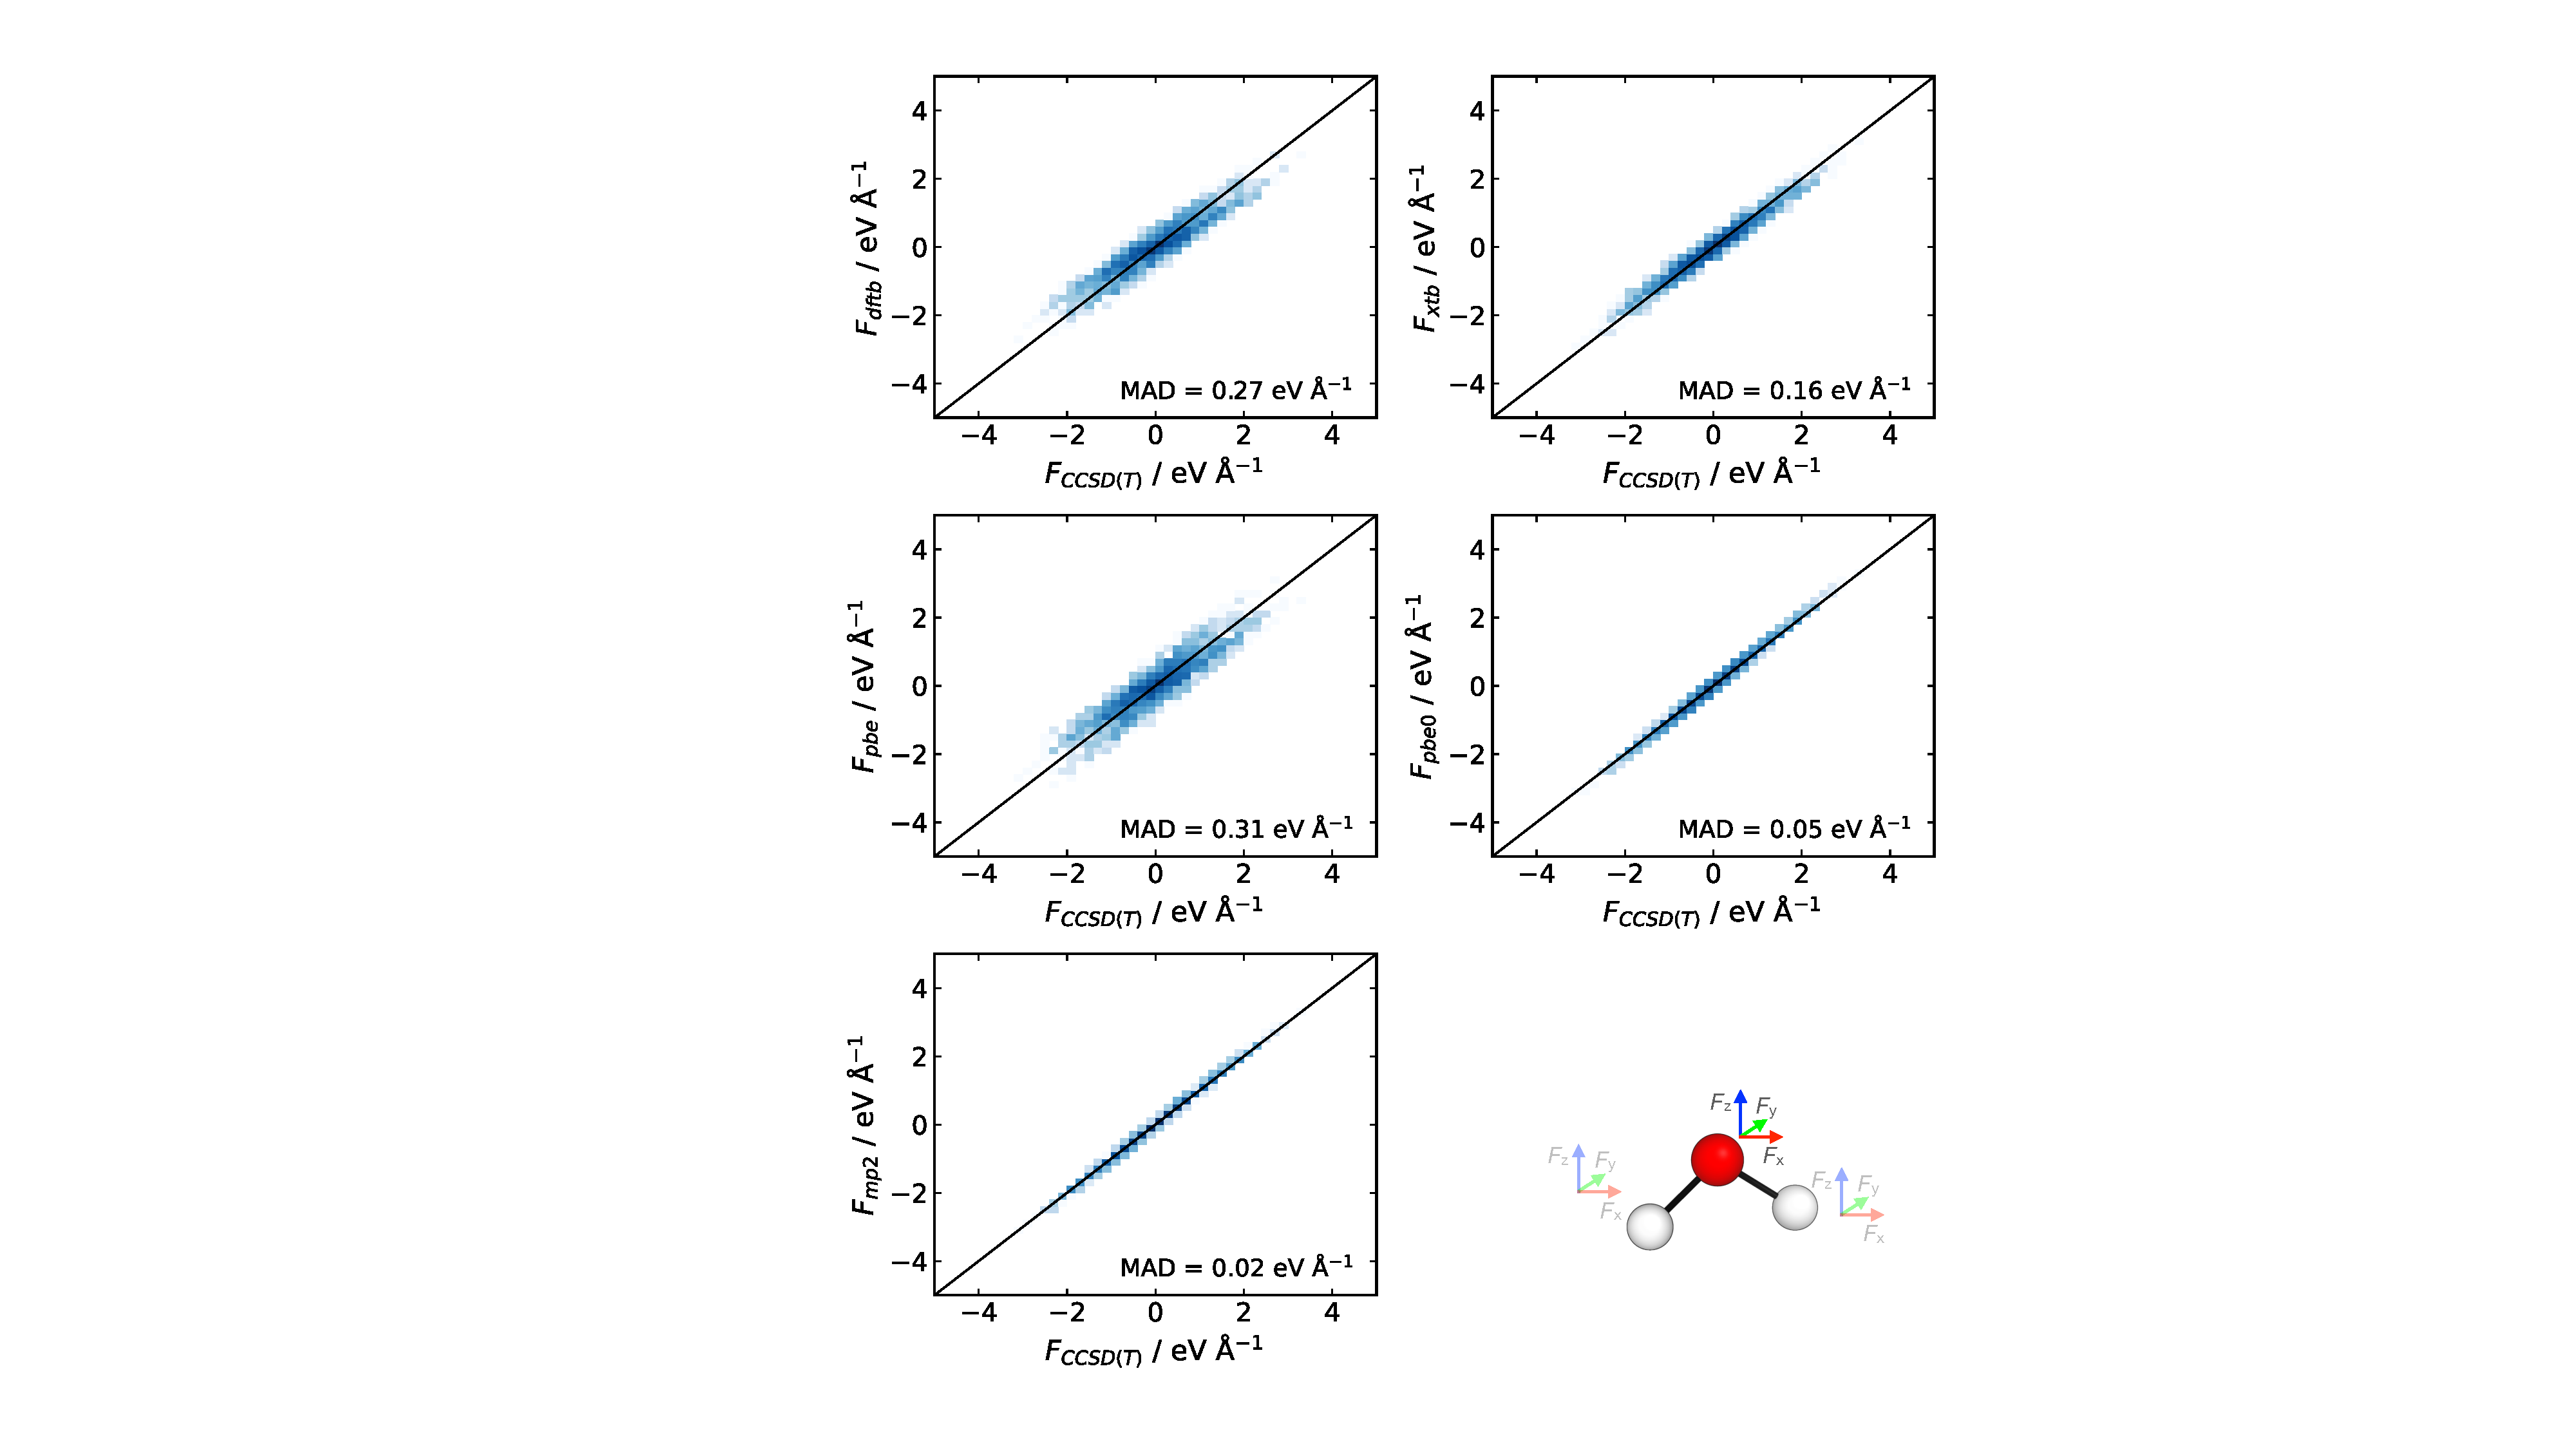
\includegraphics[width=0.76\textwidth]{figSX8.pdf}
	\vspace{0.1cm}
	\hrule
	\vspace{0.1cm}
	\caption{Parity plots of the force components (log density colouring) encountered in a DFTB(3ob) MD simulation (500 K, $\delta t$ = 0.5 ps, 1 ps, 10 step print interval) of a gas phase water molecule at a QM method compared to CCSD(T)/de2-TZVP reference values. Methods: dftb $\equiv$ DFTB(3ob), xtb $\equiv$ GFN2-XTB, pbe $\equiv$ PBE/def2-SVP, PBE0 $\equiv$ PBE0/def2-SVP, mp2 $\equiv$ MP2/def2-TZVP. Dispersion is not expected to alter the forces.}
	\label{fig::SX8}
\end{figure}

Generating frames using a DFTB(3ob) MD simulation and evaluating the force components at several levels of theory  suggests that using hybrid DFT or MP2 forces in combination with CCSD(T) energies should be sufficient to train a CCSD(T)-quality GAP. The average error is less than or similar to an `expected error' in the forces that optimises the active learning rate ($\sigma_F = <0.1$ eV \AA${}^{-1}$, \figurename{ \ref{fig::SX8}}). 


\subsection{Methane}
Training a GAP on CCSD(T) energies and MP2 forces for a gas-phase methane molecule is sufficient to generate a GAP within 1 \kcal~of the true CC surface. Using active learning at XTB to sample the configuration space, MP2 forces and CC energies, highly accurate methane dynamics (\figurename{ \ref{fig::SX10}}) can be propagated in just 5 minutes of training time (10 cores).


\begin{figure}[h!]
	\centering
	\vspace{0.4cm}
	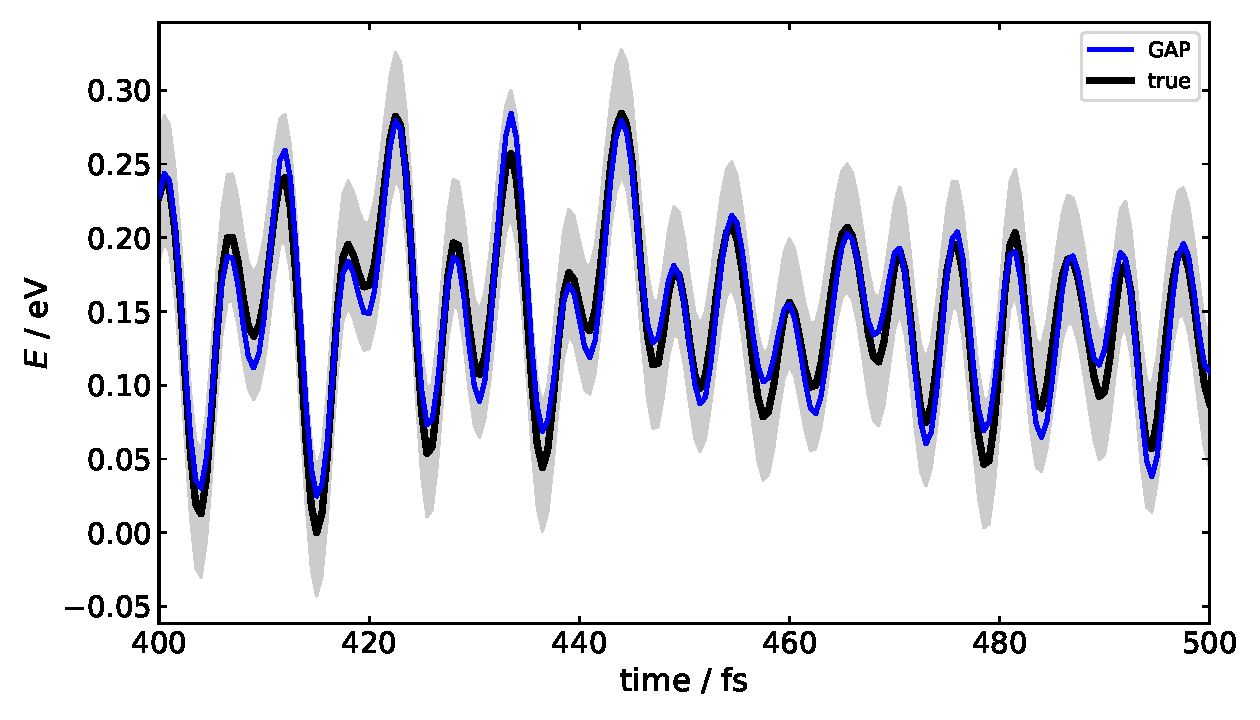
\includegraphics[height=6.4cm]{figSX10.pdf}
	\vspace{0.1cm}
	\hrule
	\vspace{0.1cm}
	\caption{GAP predicted energies compared to true CCSD(T)/def2-TZVP values for a GAP trained using GFN2-XTB active learning, MP2/def2-TZVP energy and force evaluations then CCSD(T)/def2-TZVP single point energies on those configurations. Methane AL at 1000 K, GAP-MD at 500 K with a single frame printing interval. The shaded region bounds the 1 \kcal~area of accuracy. Hyperparameters as \tablename{ \ref{table::default_params}}.}
	\label{fig::SX10}
\end{figure}


\subsection{Methanol}

Generating a GAP using active learning (AL) in parallel can lead to an overcomplete set of configurations. This is because in the initial stages the independent MD can sample similar regions of configuration space, which in turn do not provide much information for the fit. Selecting the most diverse set of configurations is therefore advantageous when the energy and forces are going to be reevaluated. Training a GAP for methanol using XTB AL then evaluating MP2/def2-TZVP energies and gradients using different number of CUR\supercite{Mahoney2009} selected configurations on the SOAP kernel matrix leads a reasonably stable \tacc~with the number selected (\tablename{ \ref{table::SX1}}).

\begin{table}[h!]
	\def\arraystretch{1.3}
	\begin{tabularx}{\textwidth}{YY}
		\hline
		$N_\text{configs}$ &\tacc~/ fs \\
		\hline
		190	   &  1000 $\pm$ 0\\
		160	   &  1000 $\pm$ 0\\
		130	   &  1000 $\pm$ 0\\
		100	   &  1000 $\pm$ 0\\
		 70	   &  1000 $\pm$ 0\\
		 40	   &  100 $\pm$ 30
	\end{tabularx}
	\hrule
	\vspace{0.1cm}
	\caption{GAP accuracy on CUR selected configurations generated as \figurename{ \ref{fig::SX10}} for methanol values are averages over three \tacc~evaluations and errors in standard error of the mean.}
	\label{table::SX1}
\end{table}


\subsection{Acetic acid}

Employing both mixed energy and forces and CUR selection of the configurations allows dynamics broadly within (MAD = 0.7 \kcal) chemical accuracy to the ground truth CC using only 167 configurations. For comparison this is $\sim 100$  times fewer CC calculations than would have been required using numerical gradients on the whole set of configurations.\footnote{334 configurations $\times$ 3 Cartesian coordinates $\times$ 2 for central differences $\times$ 8 atoms = 16,032 total calculations.} 


\begin{figure}[h!]
	\centering
	\vspace{0.4cm}
	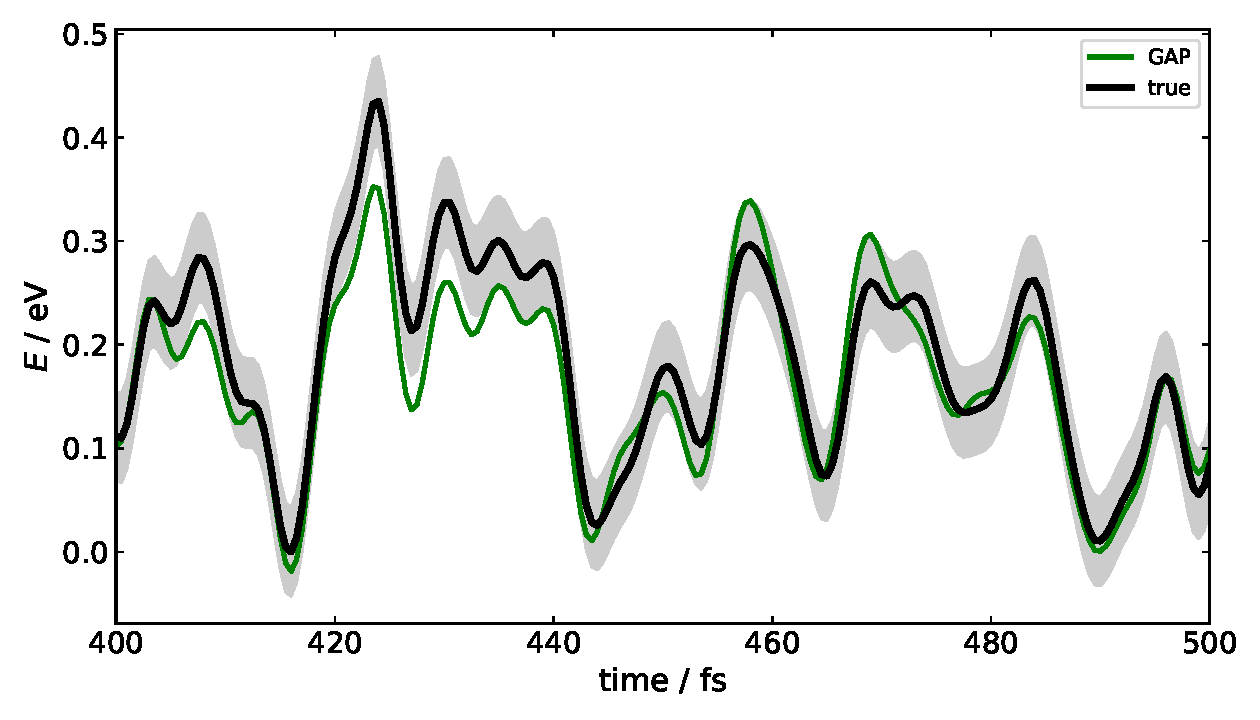
\includegraphics[height=6.4cm]{figSX11.pdf}
	\vspace{0.1cm}
	\hrule
	\vspace{0.1cm}
	\caption{As \figurename{ \ref{fig::SX10}} for acetic acid using a 50\% CUR selection of configurations. Hyperparameters as \tablename{ \ref{table::default_params}}.}
	\label{fig::SX11}
\end{figure}





\clearpage
\section{Ethene + Butadiene}  \label{section::SI_ethene_butadiene}
\subsection{Sampling Methodology}

We have shown previously that the AL sampling method (e.g. DFT functional) is important in obtaining accurate uplifted GAPs,\supercite{gaptrain2021} where the energy/forces of generated configurations are recalculated at a higher level. For the [4+2] Diels-Alder reaction between ethene and butadiene, sampling using a cheaper method than PBE does not seem to be suitable over the intrinsic reaction coordinate (IRC, \figurename{ \ref{fig::SX12}}a). Although the thermodynamics at PBE are closer to the reference MP2 values, kinetics at PBE0 are slightly closer (\figurename{ \ref{fig::SX12}}b). Sampling is therefore performed with the more transferable PBE0 functional.


\begin{figure}[h!]
	\centering
	\vspace{0.4cm}
	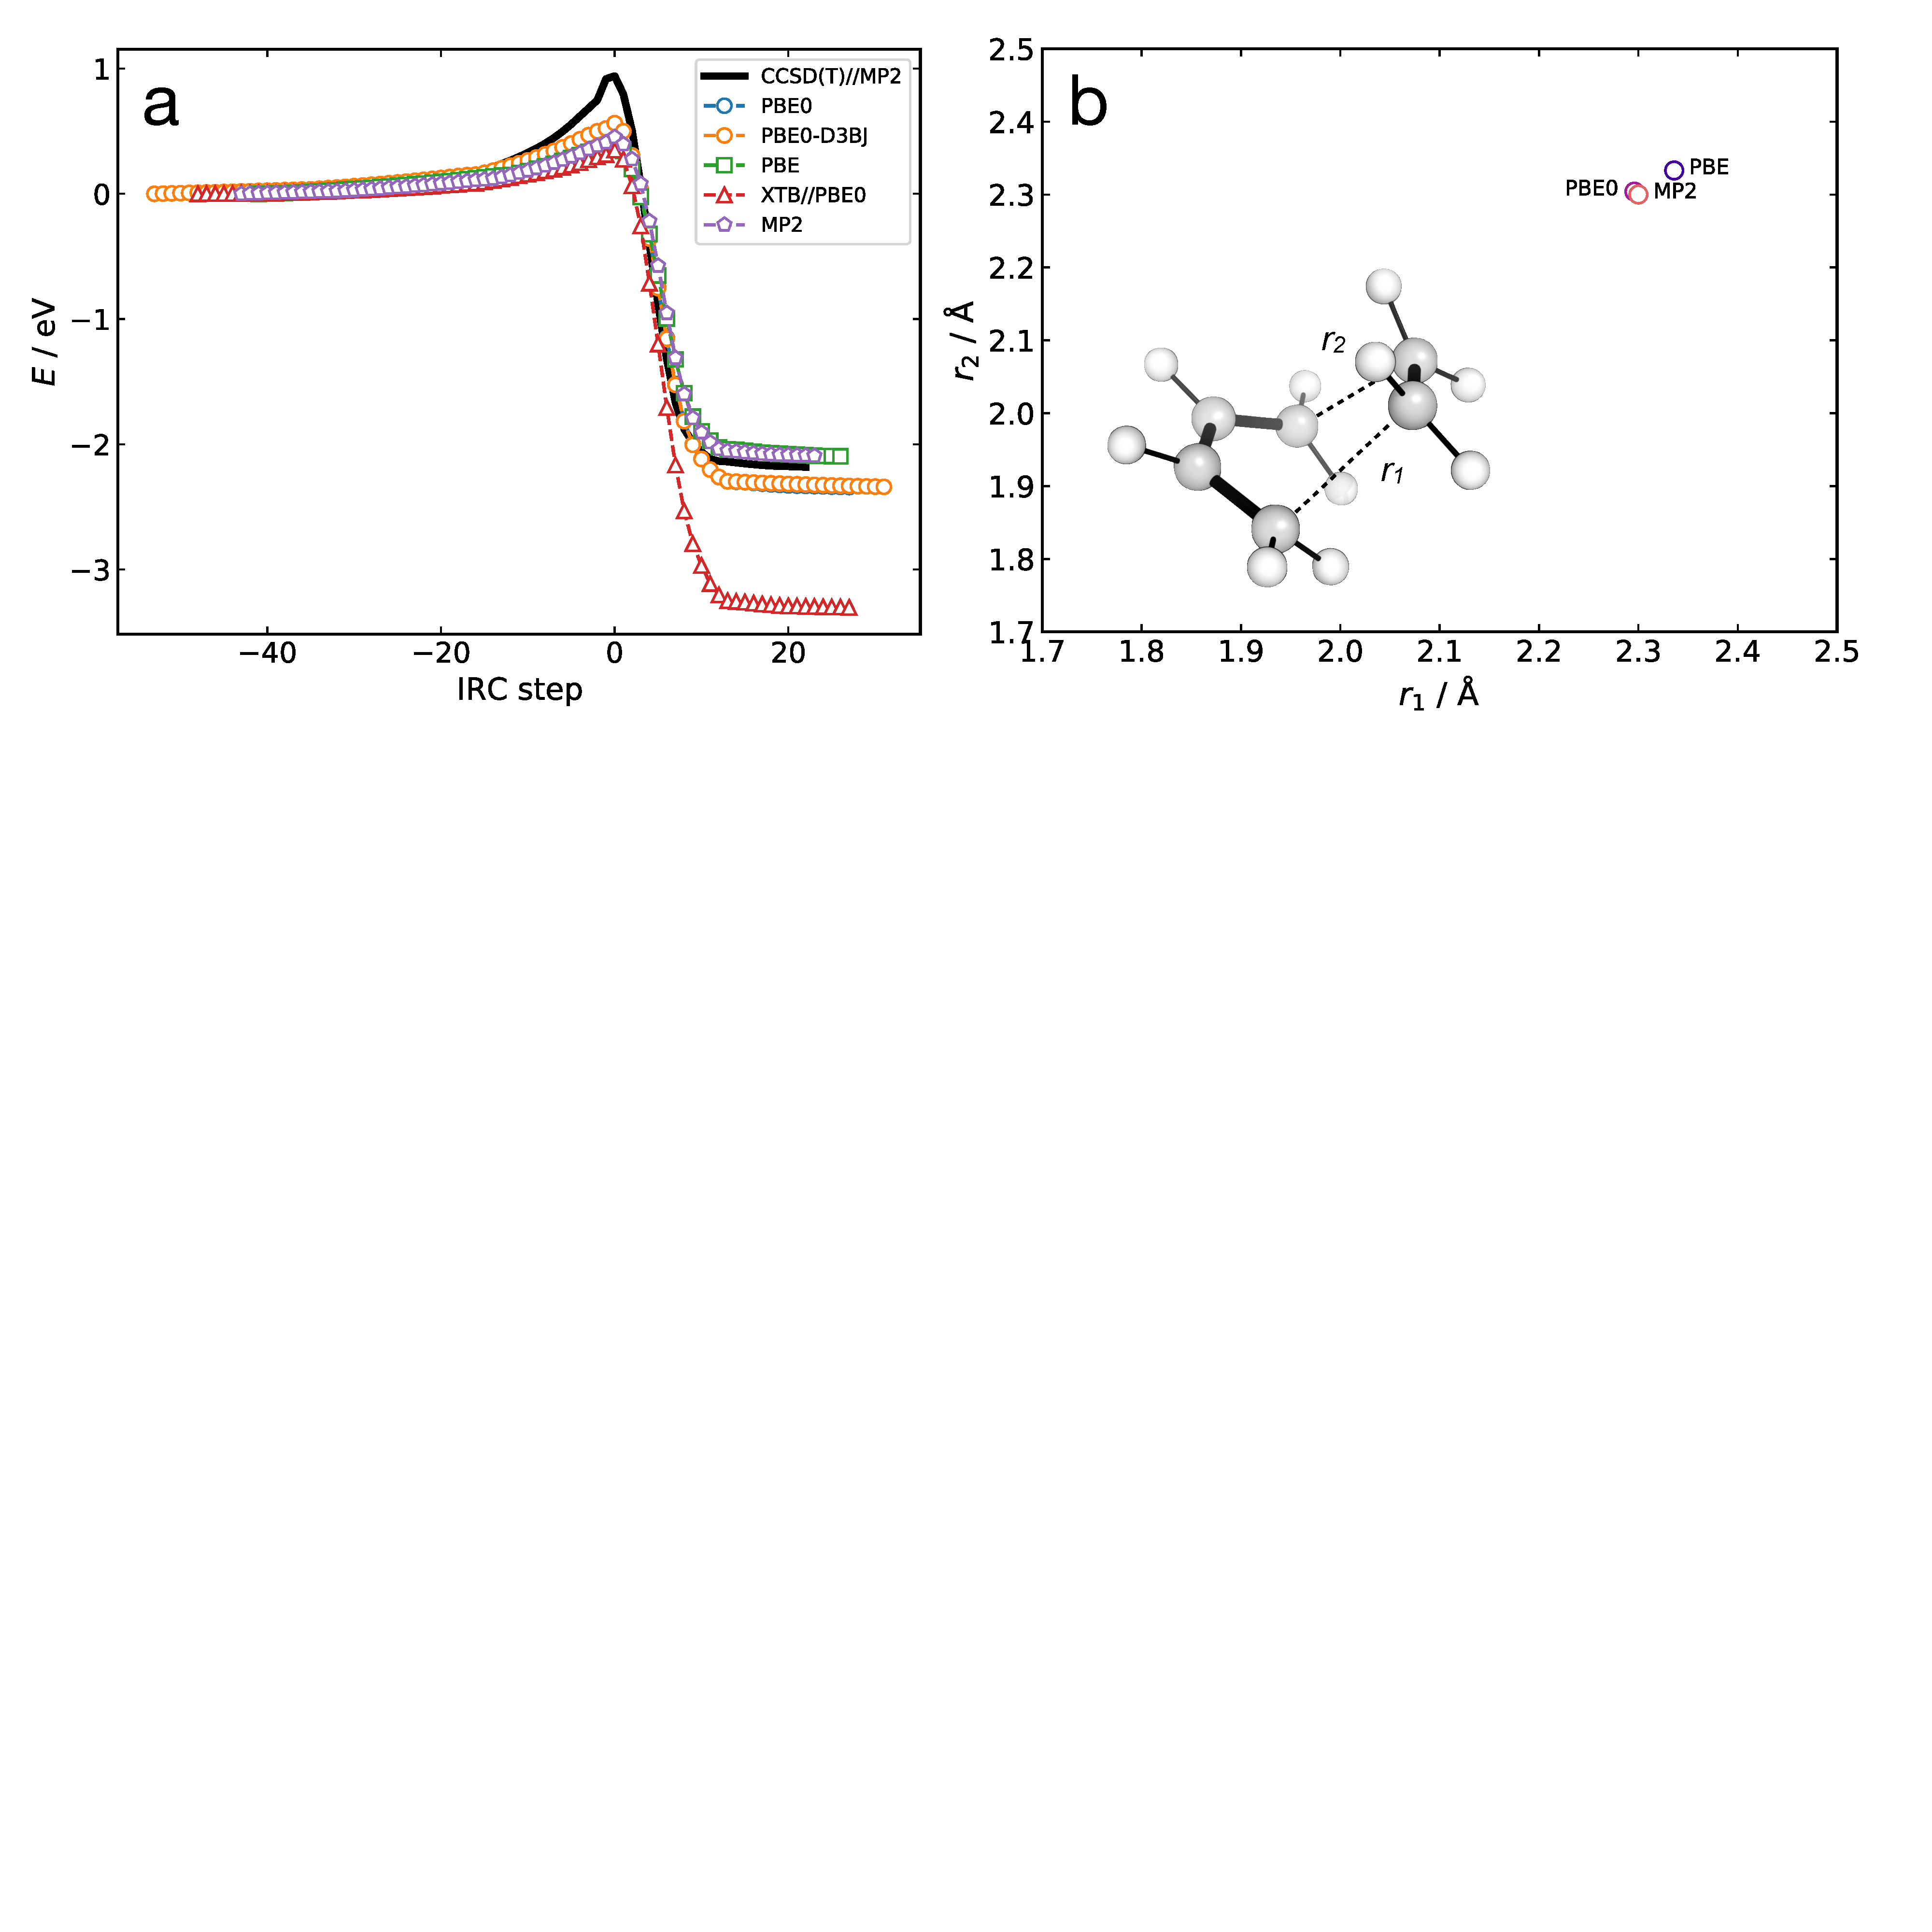
\includegraphics[width=\textwidth]{figSX12.pdf}
	\vspace{0.0cm}
	\hrule
	\vspace{0.1cm}
	\caption{Intrinsic reaction coordinates for ethene+butadiene [4+2] cyclisation at different levels of theory. DFT use def2-SVP basis sets, MP2 a def2-TZVP basis and XTB//PBE0 corresponds to GNF2-XTB energies on PBE0 IRC geometries. All TSs are confirmed as such by the presence of a single imaginary mode.}
	\label{fig::SX12}
\end{figure}


Instead of using the difference between reference and predicted energies as the criteria for adding new configurations in the AL loop the GP variance may also be used.\cite{gaptrain2021} For this system, using a threshold around $2 \times10^{-5}$ eV atom${}^{-1}$ samples in a similar region of the energy space as using a 0.09 eV (2 \kcal) difference threshold (\figurename{ \ref{fig::SX15}}), but at a much lower computational cost.\footnote{Using a `diff' strategy requires evaluating $|E_0 - E_\text{GAP}|$ at intermediate points in the GAP-MD trajectory, which are avoided using `gp\_var'.} Therefore, a `gp\_var' sampling strategy will be used for maximum training efficiency.

\begin{figure}[h!]
	\centering
	\vspace{0.4cm}
	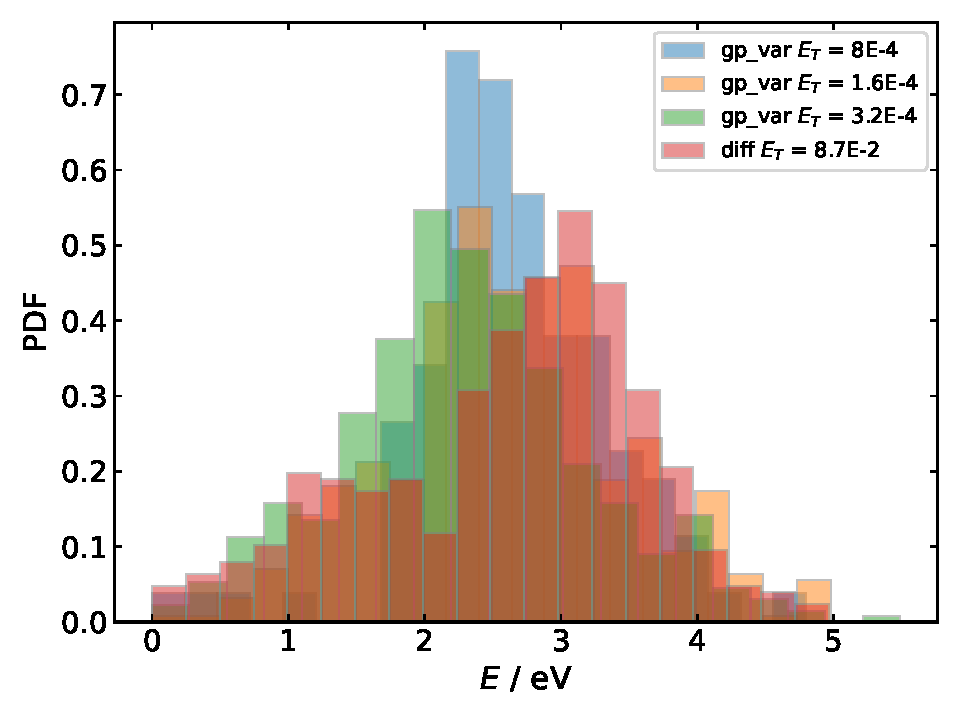
\includegraphics[height=6.4cm]{figSX15.pdf}
	\vspace{0.1cm}
	\hrule
	\vspace{0.1cm}
	\caption{Normalised probability density function over the energies sampled using AL from the ethene+butadiene [4+2] TS. gp\_var = $x$ corresponds to running GAP-MD at 500 K until the predicted variance is above $x$ eV for the whole system. diff$= y$ eV corresponds to running GAP-MD at 500 K until $|E_0 = E_\text{GAP}| > y$.}
	\label{fig::SX15}
\end{figure}

\clearpage
\subsection{Conformational Rearrangement}

\comment{
	TJW:  "interconversion differently, with an MM forcefield (GAFF), while the" - I don't understand the 'with an MM forcefield' clause
	TJW: So we see no interconversion between half-chair and chair for GAP? Do we want to run some repeats as the variation (in the MM especially) is large over 2 ps. Also 	in the caption could you mention which grey line refers to which conformation?
}

Upon cyclisation, the formed cyclohexene molecule undergoes conformational rearrangement to the more  stable (and $>99$\% populated) chair conformer. While often assumed to be fast, in cyclohexane solution the interconversion at room temperature only occurs at a rate of 55 s${}^{-1}.$\cite{Jensen1962} An MM forcefield (GAFF) affords rapid interconversion between the conformers, while the GAP (trained at 1200 K on cyclohexene) interconverts more slowly (\figurename{ \ref{fig::SX13}}). The MM however does afford the qualitatively correct distribution (\figurename{ \ref{fig::SX14}}), with the half-chair favoured over the half-boat. Developing potentials which allow for conformational changes without reparametrisation is necessary if accurate long-time simulations are to be possible.


\begin{figure}[h!]
	\centering
	\vspace{0.4cm}
	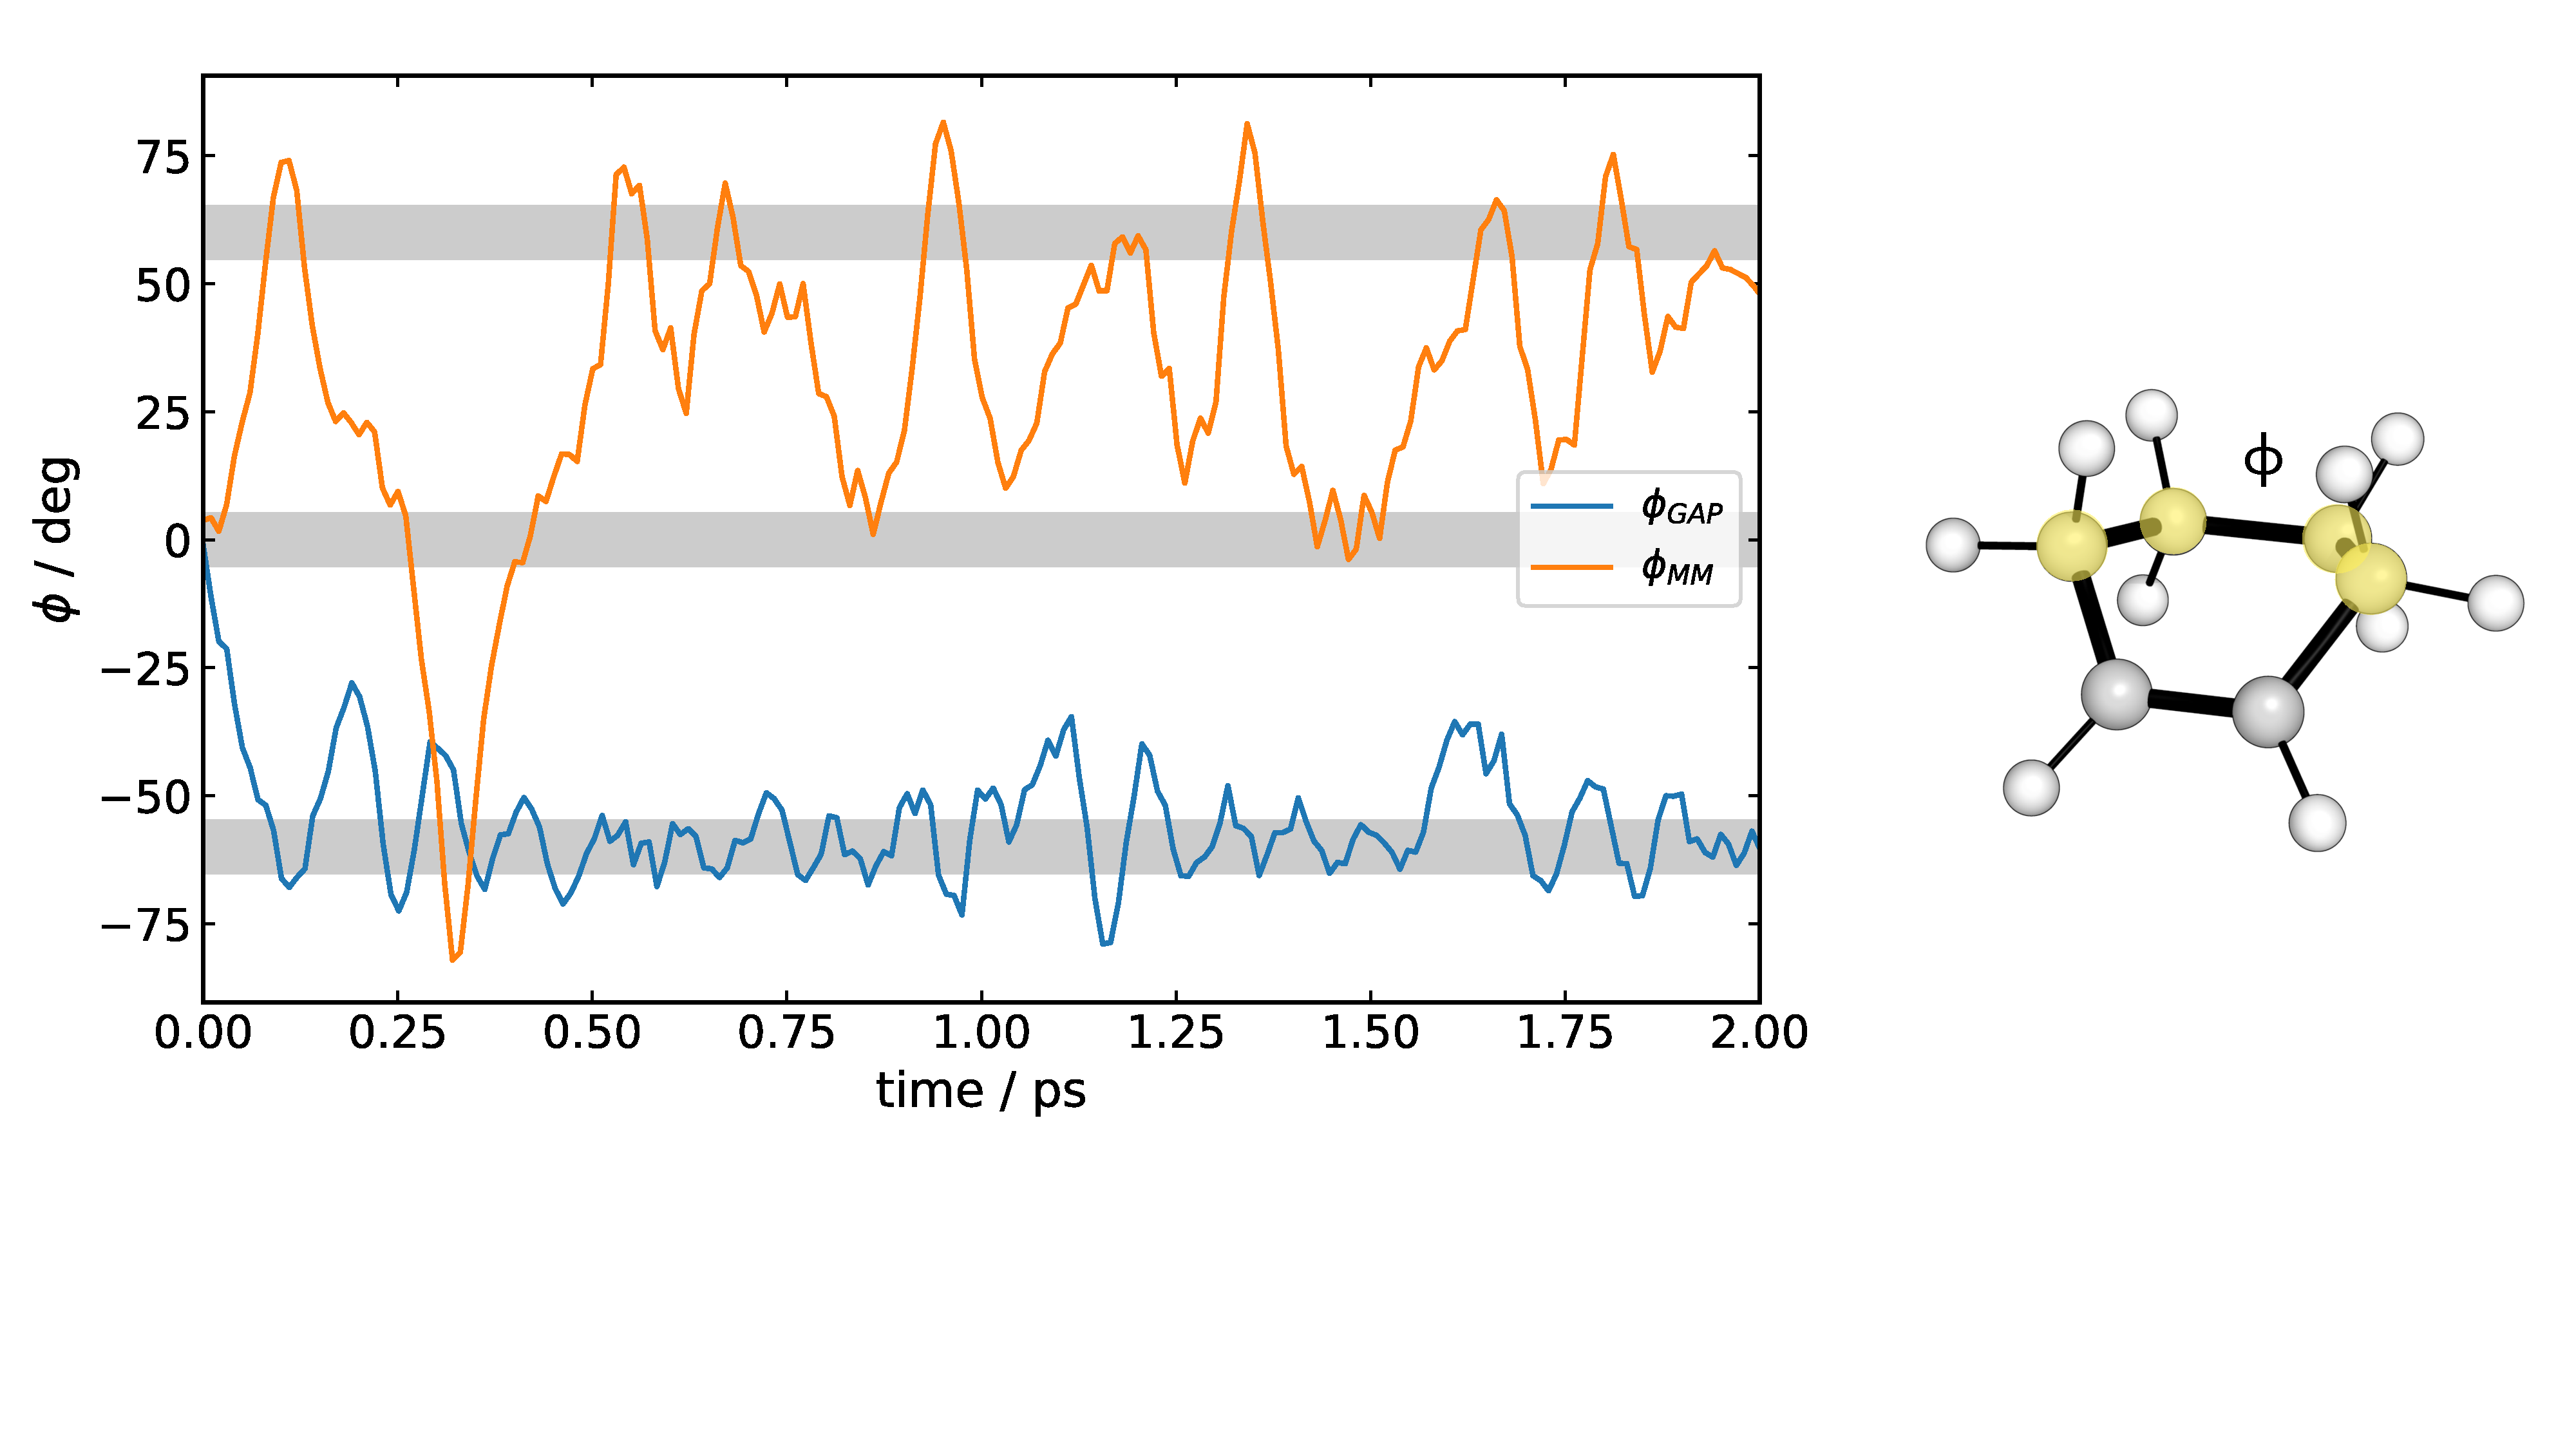
\includegraphics[width=14cm]{figSX13.pdf}
	\vspace{0.1cm}
	\hrule
	\vspace{0.1cm}
	\caption{Sample trajectories of cyclohexene at 900 K (0.5 fs timestep) using GAFF-parametrised (RESP charges) and GAP-AL generated potentials (latter uplifted from $\sim500$ GFN2-XTB AL configurations to PBE0 CUR selected to 50\%). Shaded areas highlight the approximate regions of the half-chair, boat and chair conformations of cyclohexene. Plotted using a 5 fs block average.}
	\label{fig::SX13}
\end{figure}


\begin{figure}[h!]
	\centering
	\vspace{0.4cm}
	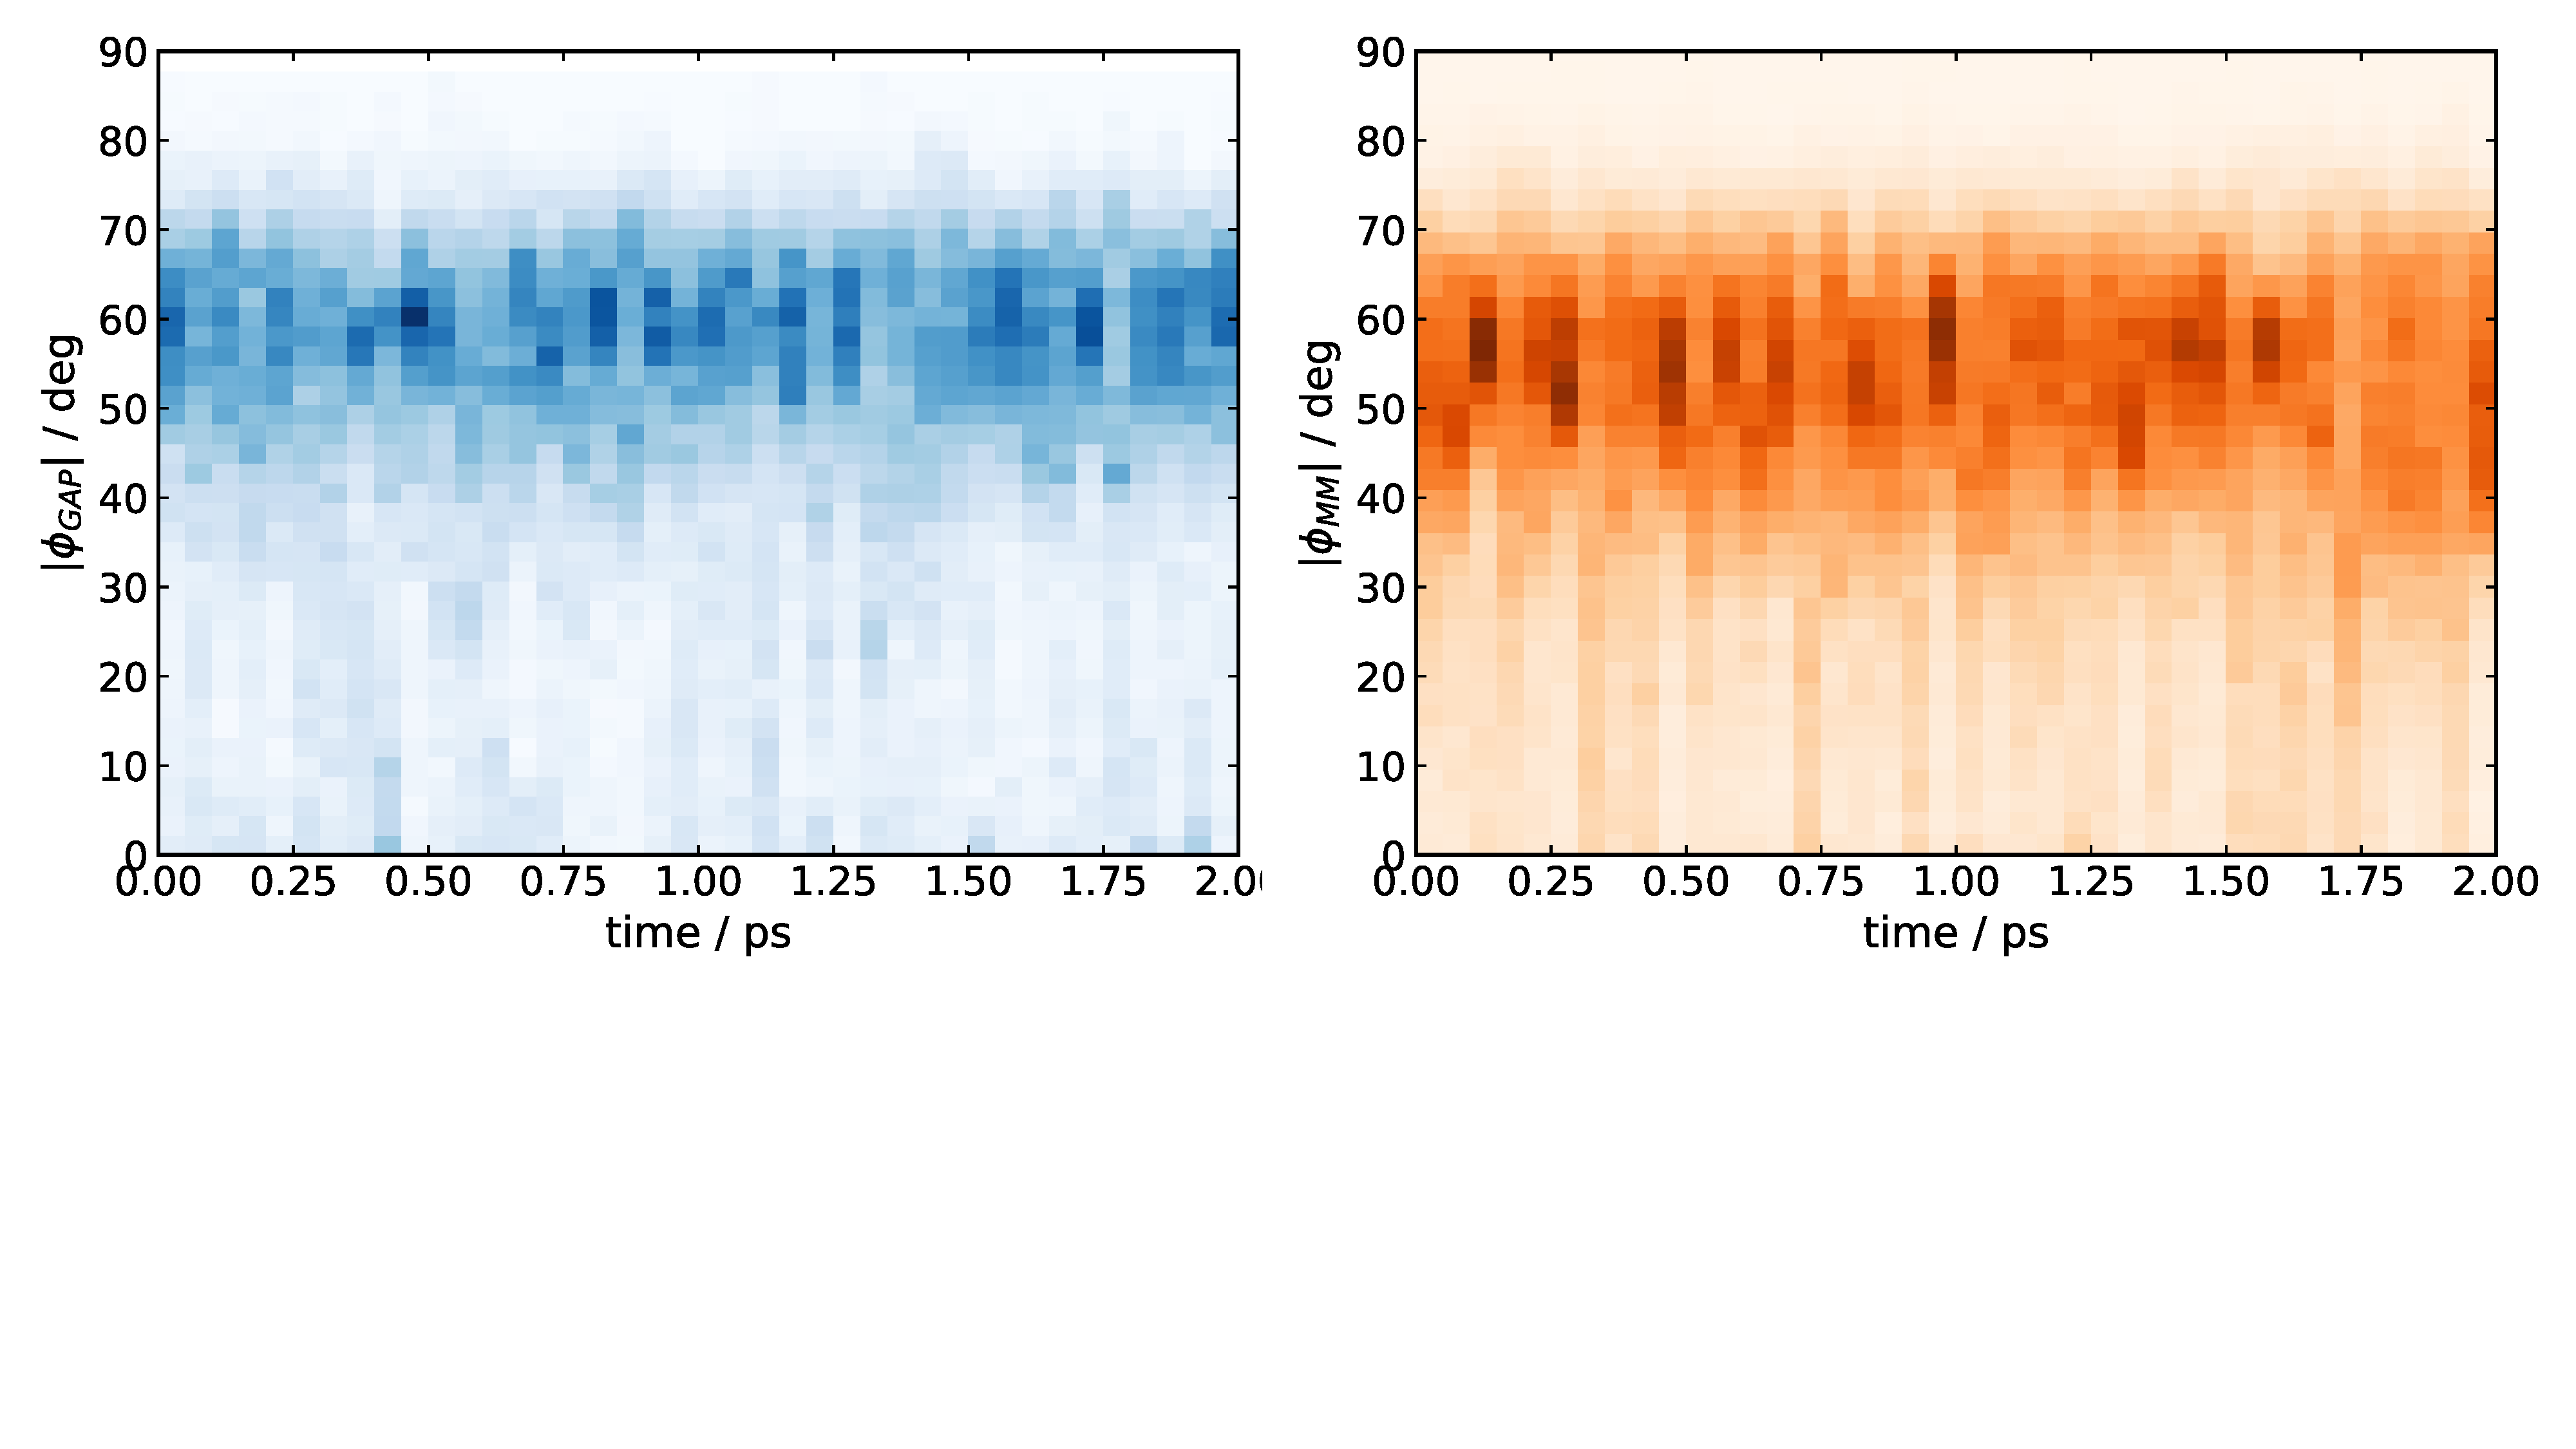
\includegraphics[width=\textwidth]{figSX14.pdf}
	\vspace{0.1cm}
	\hrule
	\vspace{0.1cm}
	\caption{Histogram of absolute dihedral angles over 100 trajectories of cyclohexene, as \figurename{ \ref{fig::SX13}}.}
	\label{fig::SX14}
\end{figure}


\clearpage
\subsection{Fragmentation}  \label{section::SI_ethene_butadiene_fragmentation}

\comment{
	TJW: The graph goes to 100, but you stop at 60. Are you going to add more t_acc for n_eval > 60?
	TY: Nope
	
	TJW: Is it worth having a graphical comparison between the t_accs for doing the I+I decomposition vs not doing it?
	TY: I hate bar charts, what do other people think?
}

With a view to reducing the number of evaluations required to generate a chemically accurate potential for ethene+butadiene cyclisation we explored an additive approach to obtaining a potential. Training the intermolecular interaction between components is an effective fragmentation of a condensed phase molecular\cite{gaptrain2021} or solid state system.\cite{Wengert2021} Extending this approach to covalent bonds however did not lead to a  gain in accuracy for a specific number of configurations (i.e. \tacc $\sim 100$ fs cf. \tacc $\sim 200$ fs using the same `gp\_var' selection strategy).

Fragmentation over a covalent bond in this manner produces two limitations (1) the intra GAP used to train the fragments may never have encountered the configuration adopted in the full system and (2) the energy scale over which the inter GAP must be accurate is much larger than without an I+I decomposition. Specifically for this system, even if the ethene and butadiene potentials are high quality ($\tau_\text{acc} > 1$ ps, \figurename{ \ref{fig::SX16}}) they will not have well sampled the pyramidal sp${}^3$ geometrics present in the  cyclohexene product. This increases the amount of data required for the inter GAP to learn. Furthermore, the intra component distortion is only possible in the product making the energy scale larger that otherwise required (\figurename{ \ref{fig::SX15}}). The one advantage is that the reactant state (reactants separated by $> 3$\AA) is well approximated by the intra+inter decomposition, as observed for e.g. bulk water.


\begin{figure}[h!]
	\centering
	\vspace{0.4cm}
	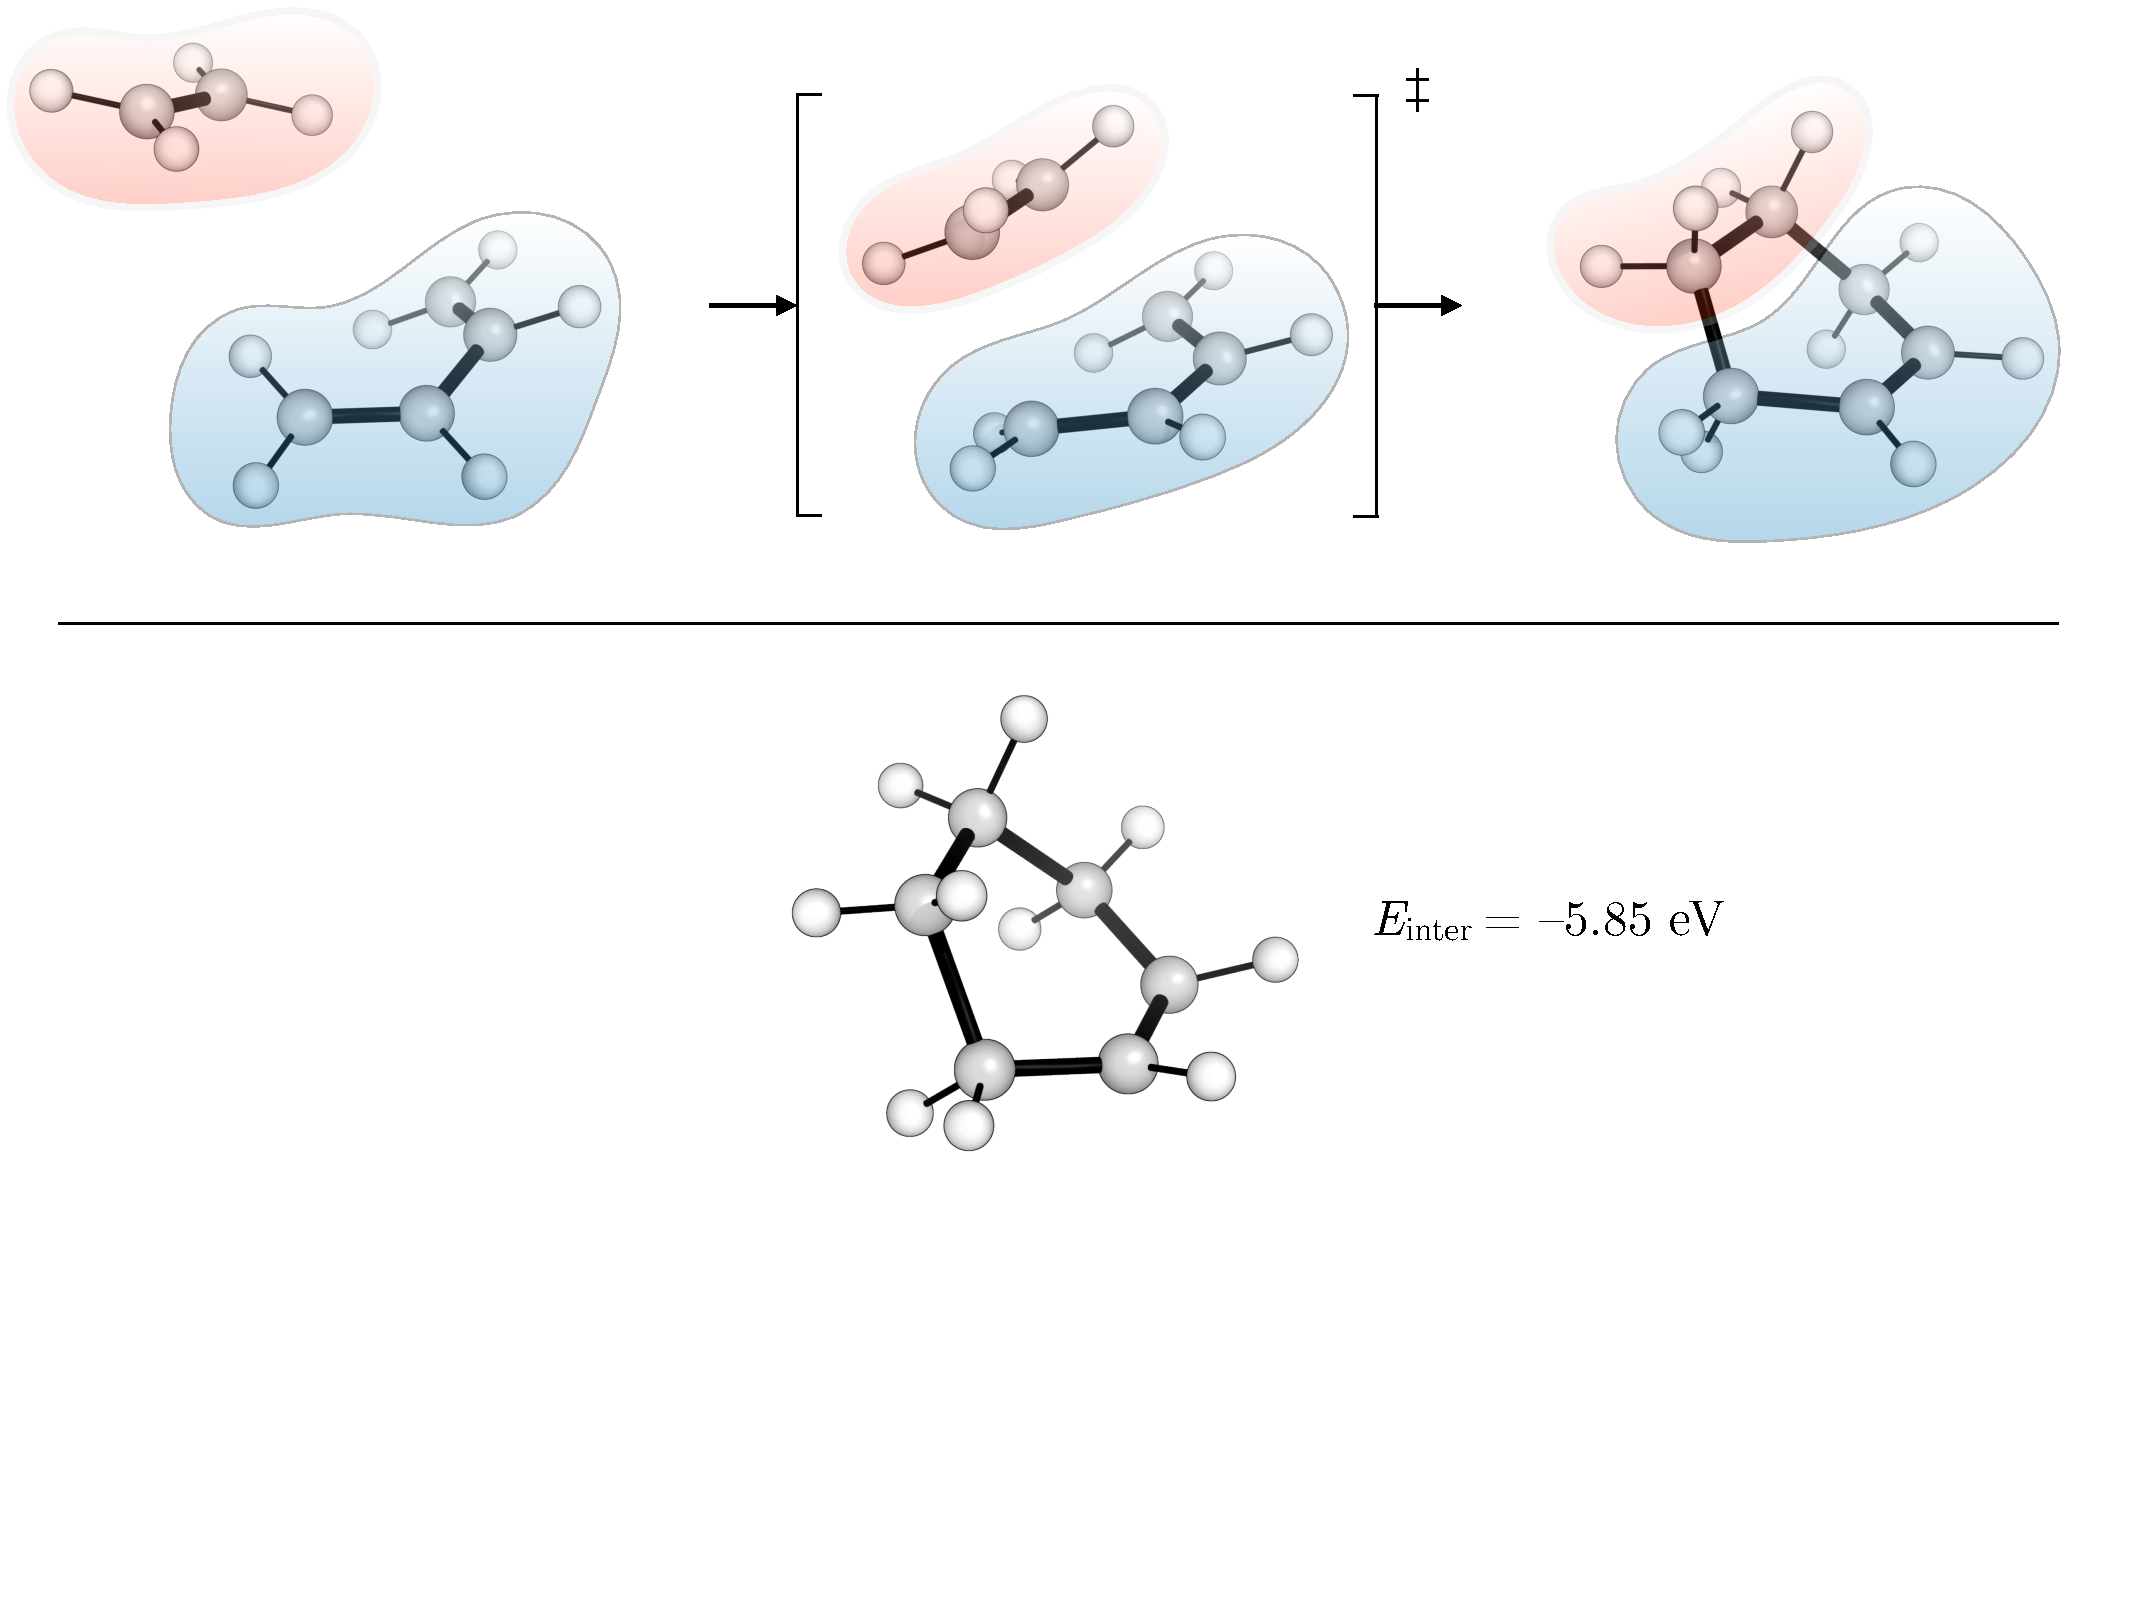
\includegraphics[width=0.9\textwidth]{figSX17.pdf}
	\vspace{0.1cm}
	\hrule
	\vspace{0.1cm}
	\caption{Sample intra+inter fragmentation strategy for ethene+butadiene. An example configuration is highlighted in the bottom panel along with the residual interaction energy between the two fragments (i.e. true total energy minus $E_\text{intra}^\text{GAP}$) for each component.}
	\label{fig::SX17}
\end{figure}


\begin{figure}[h!]
	\centering
	\vspace{0.4cm}
	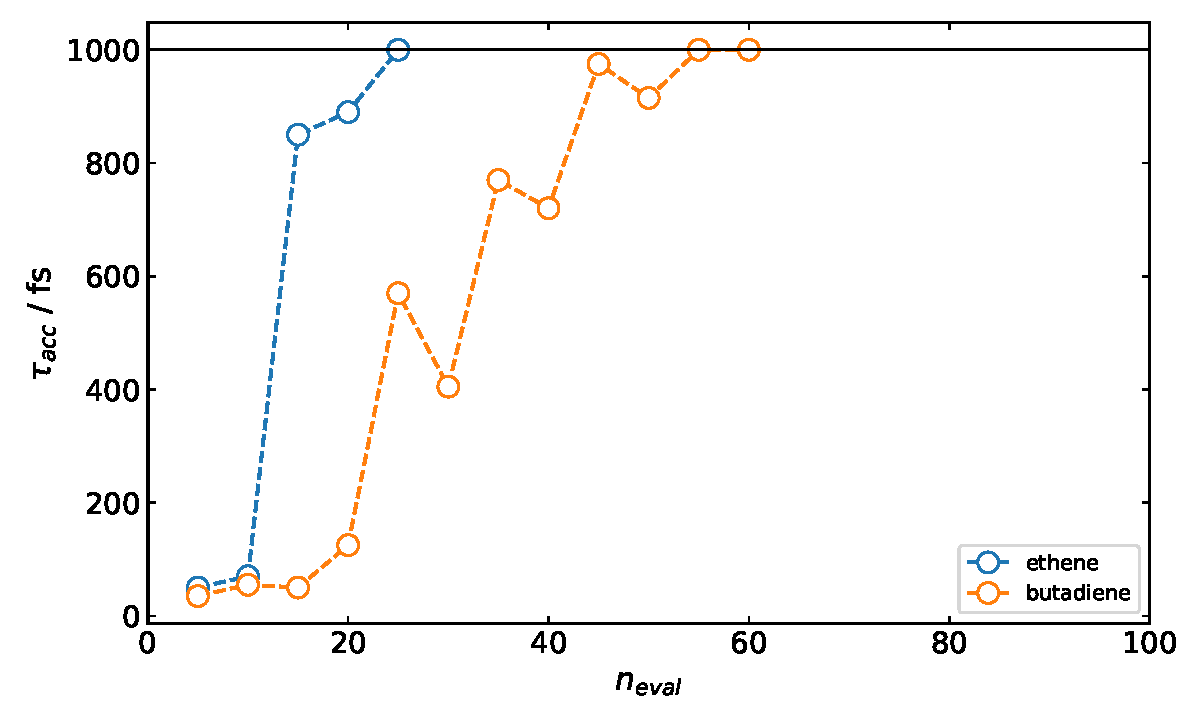
\includegraphics[height=6.4cm]{figSX16.pdf}
	\vspace{0.1cm}
	\hrule
	\vspace{0.1cm}
	\caption{Learning curves for ethene and butadiene using a `gp\_var' selection strategy with $E_t = 1\times10^{-5}$ eV atom${}^{-1}$. $\tau_\text{acc}$ uses $E_l$ = 1 \kcal, $E_T = 10E_l$, 25 fs interval and a maximum time of 1 ps. $n_\text{eval}$ is the total number of reference PBE0/def2-SVP calculations performed.}
	\label{fig::SX16}
\end{figure}


\subsection{Reaction Training}

Training a GAP for the whole ethene+butadiene reaction with the optimised hyperparameters (\tablename{ \ref{table::updated_params}}) from the TS using a `gp\_var' selection strategy generated a MLP capable of a \tacc~$\sim 500$ fs at 1 \kcal. A representative trajectory back and forwards from the TS illustrates the achieved accuracy (\figurename{ \ref{fig::SX22}}) available in just 30 CPUh.


\begin{figure}[h!]
	\centering
	\vspace{0.4cm}
	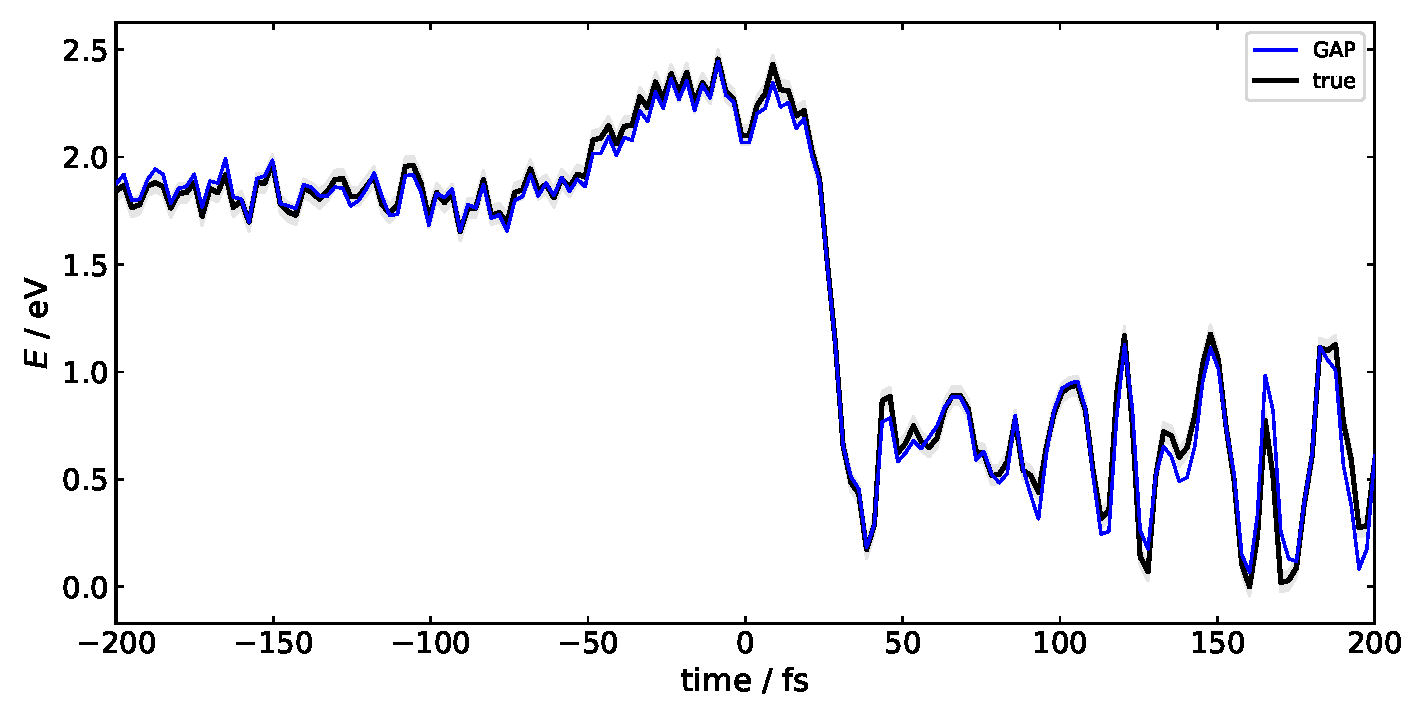
\includegraphics[height=6.4cm]{figSX22.pdf}
	\vspace{0.1cm}
	\hrule
	\vspace{0.1cm}
	\caption{Comparison of true (PBE0/def2-SVP) and GAP predicted energies over one trajectory propagated from the TS to reactants ($t < 0$) and products ($t > 0$). GAP trained using `gp\_var' ($E_t = 2\times10^{-5}$ eV \AA${}^{-1}$, 300 K) and contained 181 configurations.}
	\label{fig::SX22}
\end{figure}


%%%%%%%%%%%%%%%%%%%%%%%%%%%%%%%%%%%%%
%   Old data not using the correct hyperparameters
%%%%%%%%%%%%%%%%%%%%%%%%%%%%%%%%%%%%%
\comment{

\subsection{Different Training Strategies}


The following section provides details of how modifying training hyperparameters affects \tacc~(300 K simulation from the ethene +butadiene [4+2] TS, $E_l$ = 1 \kcal, $E_t = 10E_l$). As random initialisation can have a moderate ($\sim50$\%) impact on the calculated \tacc, they are averaged over 3 independent repeats of the whole training strategy (\tablename{ \ref{table::SX2}}).


\begin{table}[h!]
	\def\arraystretch{1.3}
	\begin{tabularx}{\textwidth}{YYYYYYY}
		\hline
		Initial config.(s)& AL strategy & $E_T$ / eV & $t_\text{max}$ / ps& $T$ / K &other &\tacc~ / fs \\
		\hline
		 & I+I, diff& 0.0867& 1& intra: 1000, inter: 500& -& 155\\
		TS + separated reactants & I+I, gp\_var & 1.6 $\times10^{-4}$& 1& intra: 1000, inter: 300& -& 112\\
		TS + separated reactants & I+I, gp\_var& 8 $\times10^{-4}$& 5& intra: 500, inter: 300& -& $<25$\\
		& I+I, gp\_var& intra: 1.6 $\times10^{-4}$, inter: 4.8 $\times10^{-4}$& 1& intra: 1000, inter: 500& -& 37\\
		\hline
		Product & uphill {\footnotesize{(2 eV bond${}^{-1}$)}}, gp\_var& 8 $\times10^{-4}$& 5 & 500 & - & 78 \\
		TS & gp\_var & 1.6$\times10^{-4}$ & 0.5 & 300 & - & 182 \\
		TS & gp\_var & 3.2$\times10^{-4}$ & 0.5 & 300 & - & 162 \\
		TS & gp\_var & 3.2$\times10^{-4}$ & 0.5 & 300 & $n_\text{max}$ = 10 & 202 \\
		TS & diff & 0.0867 & 1 & 500 & - & 230 \\
		TS & diff & 0.1734 & 1 & 500 & - & 200 \\
		TS & gp\_var  & 1.6$\times10^{-4}$ & 1 & 500 & - & 180 \\
		TS & gp\_var  & 3.2$\times10^{-4}$ & 1 & 500 & - & 140 \\
		TS & gp\_var  & 3.2$\times10^{-4}$ & 0.5 & 300 & $r_c$ = 3.0 \AA& 255 \\
		TS & gp\_var  & 3.2$\times10^{-4}$ &0.5 & 300 & $r_c$ = 5.0 \AA& 150 \\
		TS & gp\_var  & 8$\times10^{-4}$ & 1 & 500 & - & 207 \\
		TS & gp\_var  & 8$\times10^{-4}$ & 1 & 1000 & - & 90 \\
		TS & gp\_var  & 8$\times10^{-4}$ & 5 & 300 & - & 215 \\
		\hline
		 & gp\_var  & 8$\times10^{-4}$ & 5 & 300 & - & 257 \\
		TS +reactant + product& gp\_var  & 8$\times10^{-4}$ & 5 & 2, 300 & - & 170 \\
		 & gp\_var  & 8$\times10^{-4}$ & 5 & 5, 50, 500 & - & 70 \\
	\end{tabularx}
	\hrule
	\vspace{0.1cm}
	\caption{Training strategies for the [4+2] cyclisation between ethene and butadiene. GAP and SOAP hyperparameters as \tablename{ \ref{table::updated_params}}. All strategies generate at most 500 configurations (for each component in I+I).}
	\label{table::SX2}
\end{table}


\clearpage
To understand the plateau in \tacc at around 200 fs for training from the TS the dependence of \tacc~on the temperature at which it is evaluated (and the potential trained) is outlined in \figurename{ \ref{fig::SX18}}. The larger configuration space assessed at higher temperatures is reflected by a reduced \tacc~, approaching that of GAPs trained from the TS in \tablename{ \ref{table::SX2}}.


\begin{figure}[h!]
	\centering
	\vspace{0.4cm}
	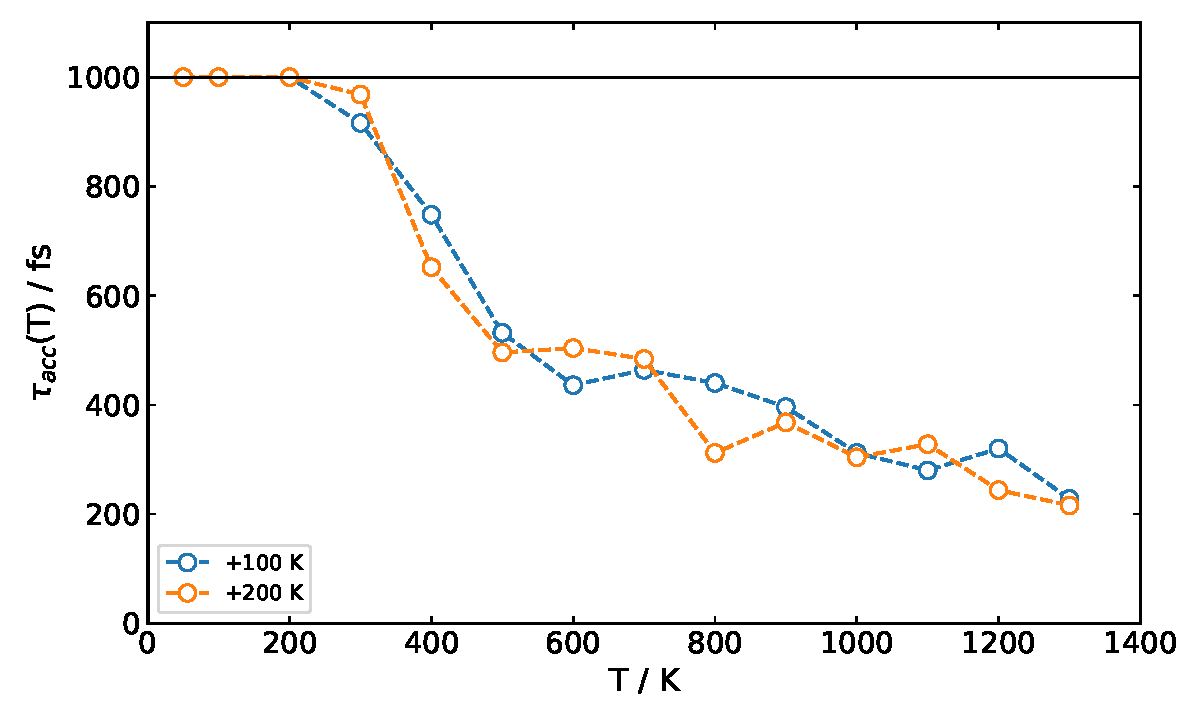
\includegraphics[height=6.4cm]{figSX18.pdf}
	\vspace{0.1cm}
	\hrule
	\vspace{0.1cm}
	\caption{\tacc for simulation of cyclohexene trained and evaluated at the GN2-XTB level of theory (0.5 fs timestep, 25 fs interval, $E_l = 1$ \kcal) at a temperature. Active learning performed using a `gp\_var' strategy ($E_T = 1.6\times10^{-4}$ eV) at either 100 K or 200 K above the temperature at which \tacc~is evaluated.}
	\label{fig::SX18}
\end{figure}

 
} % end comment

\clearpage
\section{Atomic Energy Errors}  \label{section::SI_atomic_energy_errors}

In addition to the complexity increasing with system size, the accuracy \emph{per atom} increases when the goal is to generate a potential that is accurate to 1 \kcal~in total energy. To evaluate if the total (relative) energy is an important quantity for our target properties (free energies or reaction dynamics) we use the set of S${}_N$2 reactions: Cl$^{-}$ + \{MeCl, EtCl, ${}^n$PrCl\}. 

Generating highly accurate (error $\ll 1$ \kcal) GAPs for the reaction is possible (\figurename{ \ref{fig::SX19a}}). Using these potentials and increasing the regularisation (`expected error') on energies \emph{per atom} leads to larger errors on the potential energy  barriers (\figurename{ \ref{fig::SX19b}}). Note that these GAPs are trained purely on energies, to isolate the effect of adding larger atomic errors. This scenario simulates training different potentials to the same \emph{per atom} accuracy, which -- as expected -- leads to larger errors on barriers for these small systems. Based on these data the total energy is an important quantity in predicting {\large {\color{red} free}} energy barriers.


\begin{figure}[h!]
	\centering
	\vspace{0.5cm}
	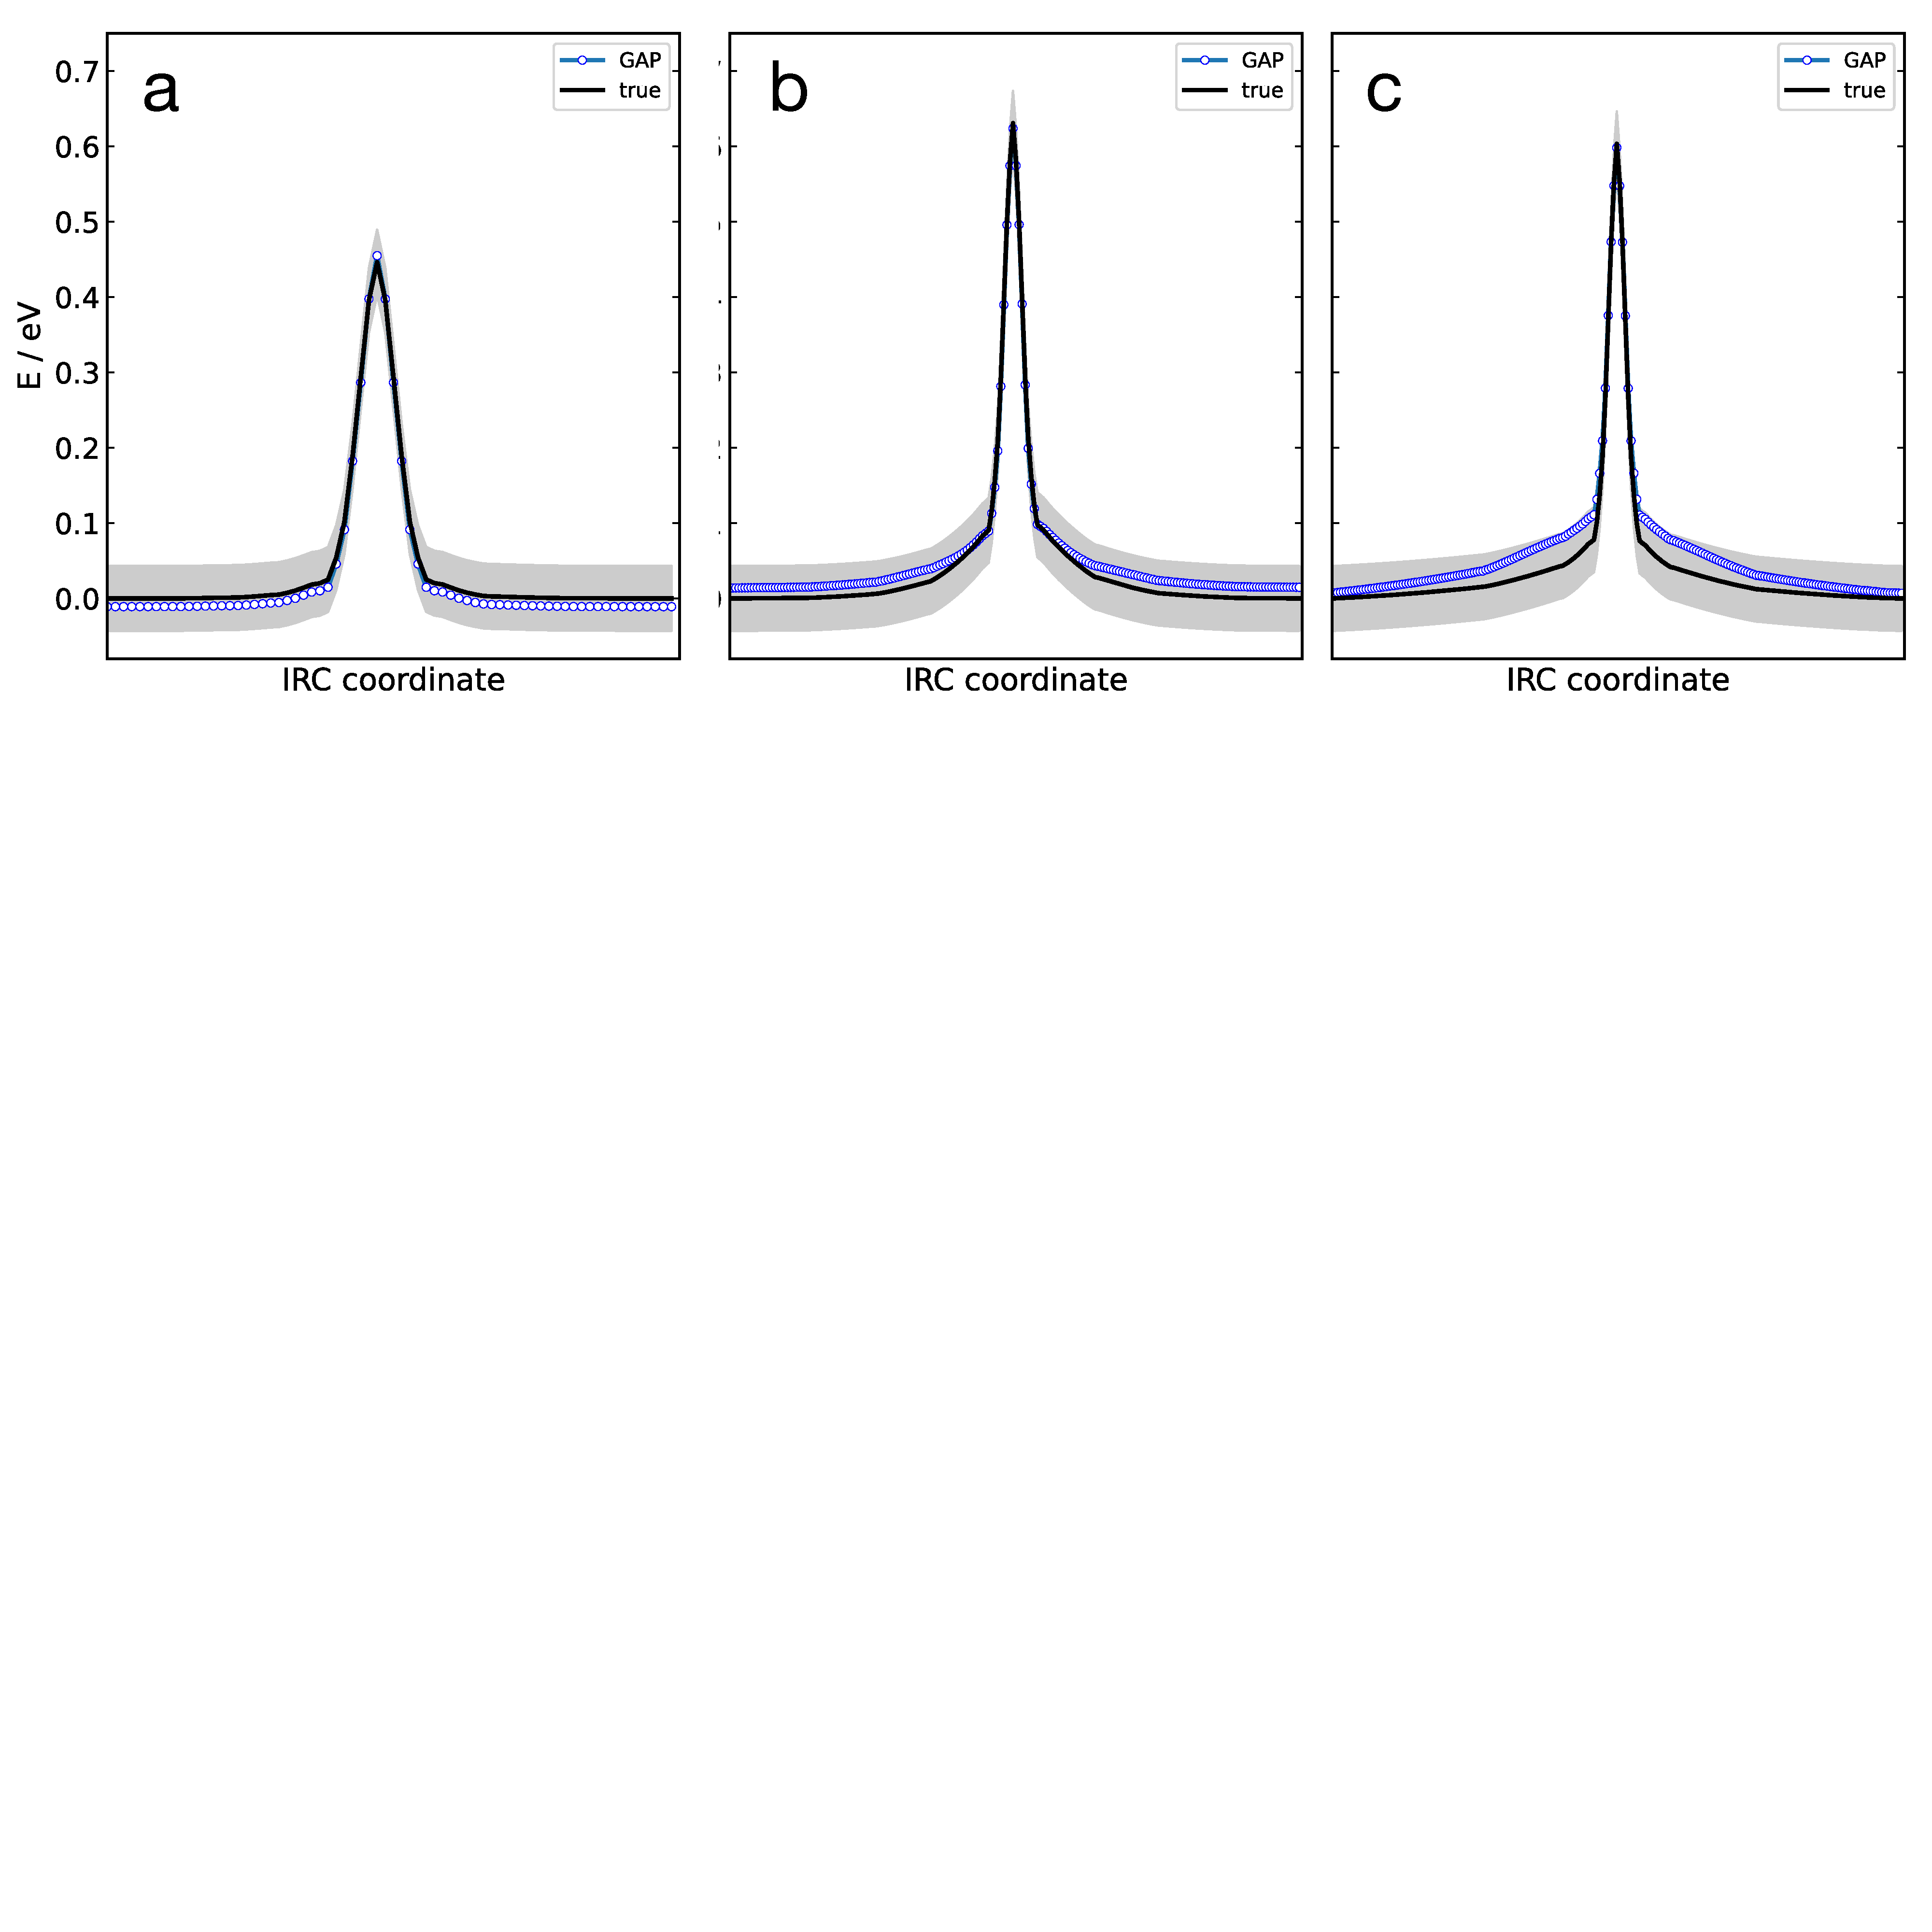
\includegraphics[width=\textwidth]{figSX19a.pdf}
	\vspace{0.1cm}
	\hrule
	\vspace{0.1cm}
	\caption{True intrinsic reaction coordinates (IRCs) for Cl$^{-}$ + MeCl, EtCl, ${}^n$PrCl  (a--c respectively), calculated at PBE0-D3BJ/ma-def2-SVP with GAP predicted values overlaid. GAPs trained at 500 K from their respective TSs up to a maximum time of 0.5 ps using a `gp\_var' strategy ($E_t = 1\times10^{-5}$ eV atom${}^{-1}$. $\sigma_E = 10^{-3.5}$ eV atom${}^{-1}$, $\sigma_F = 10^{-1.5}$ eV \AA${}^{-1}$). The shaded area bounds the 1 \kcal~region of accuracy.}
	\label{fig::SX19a}
\end{figure}


\begin{figure}[h!]
	\centering
	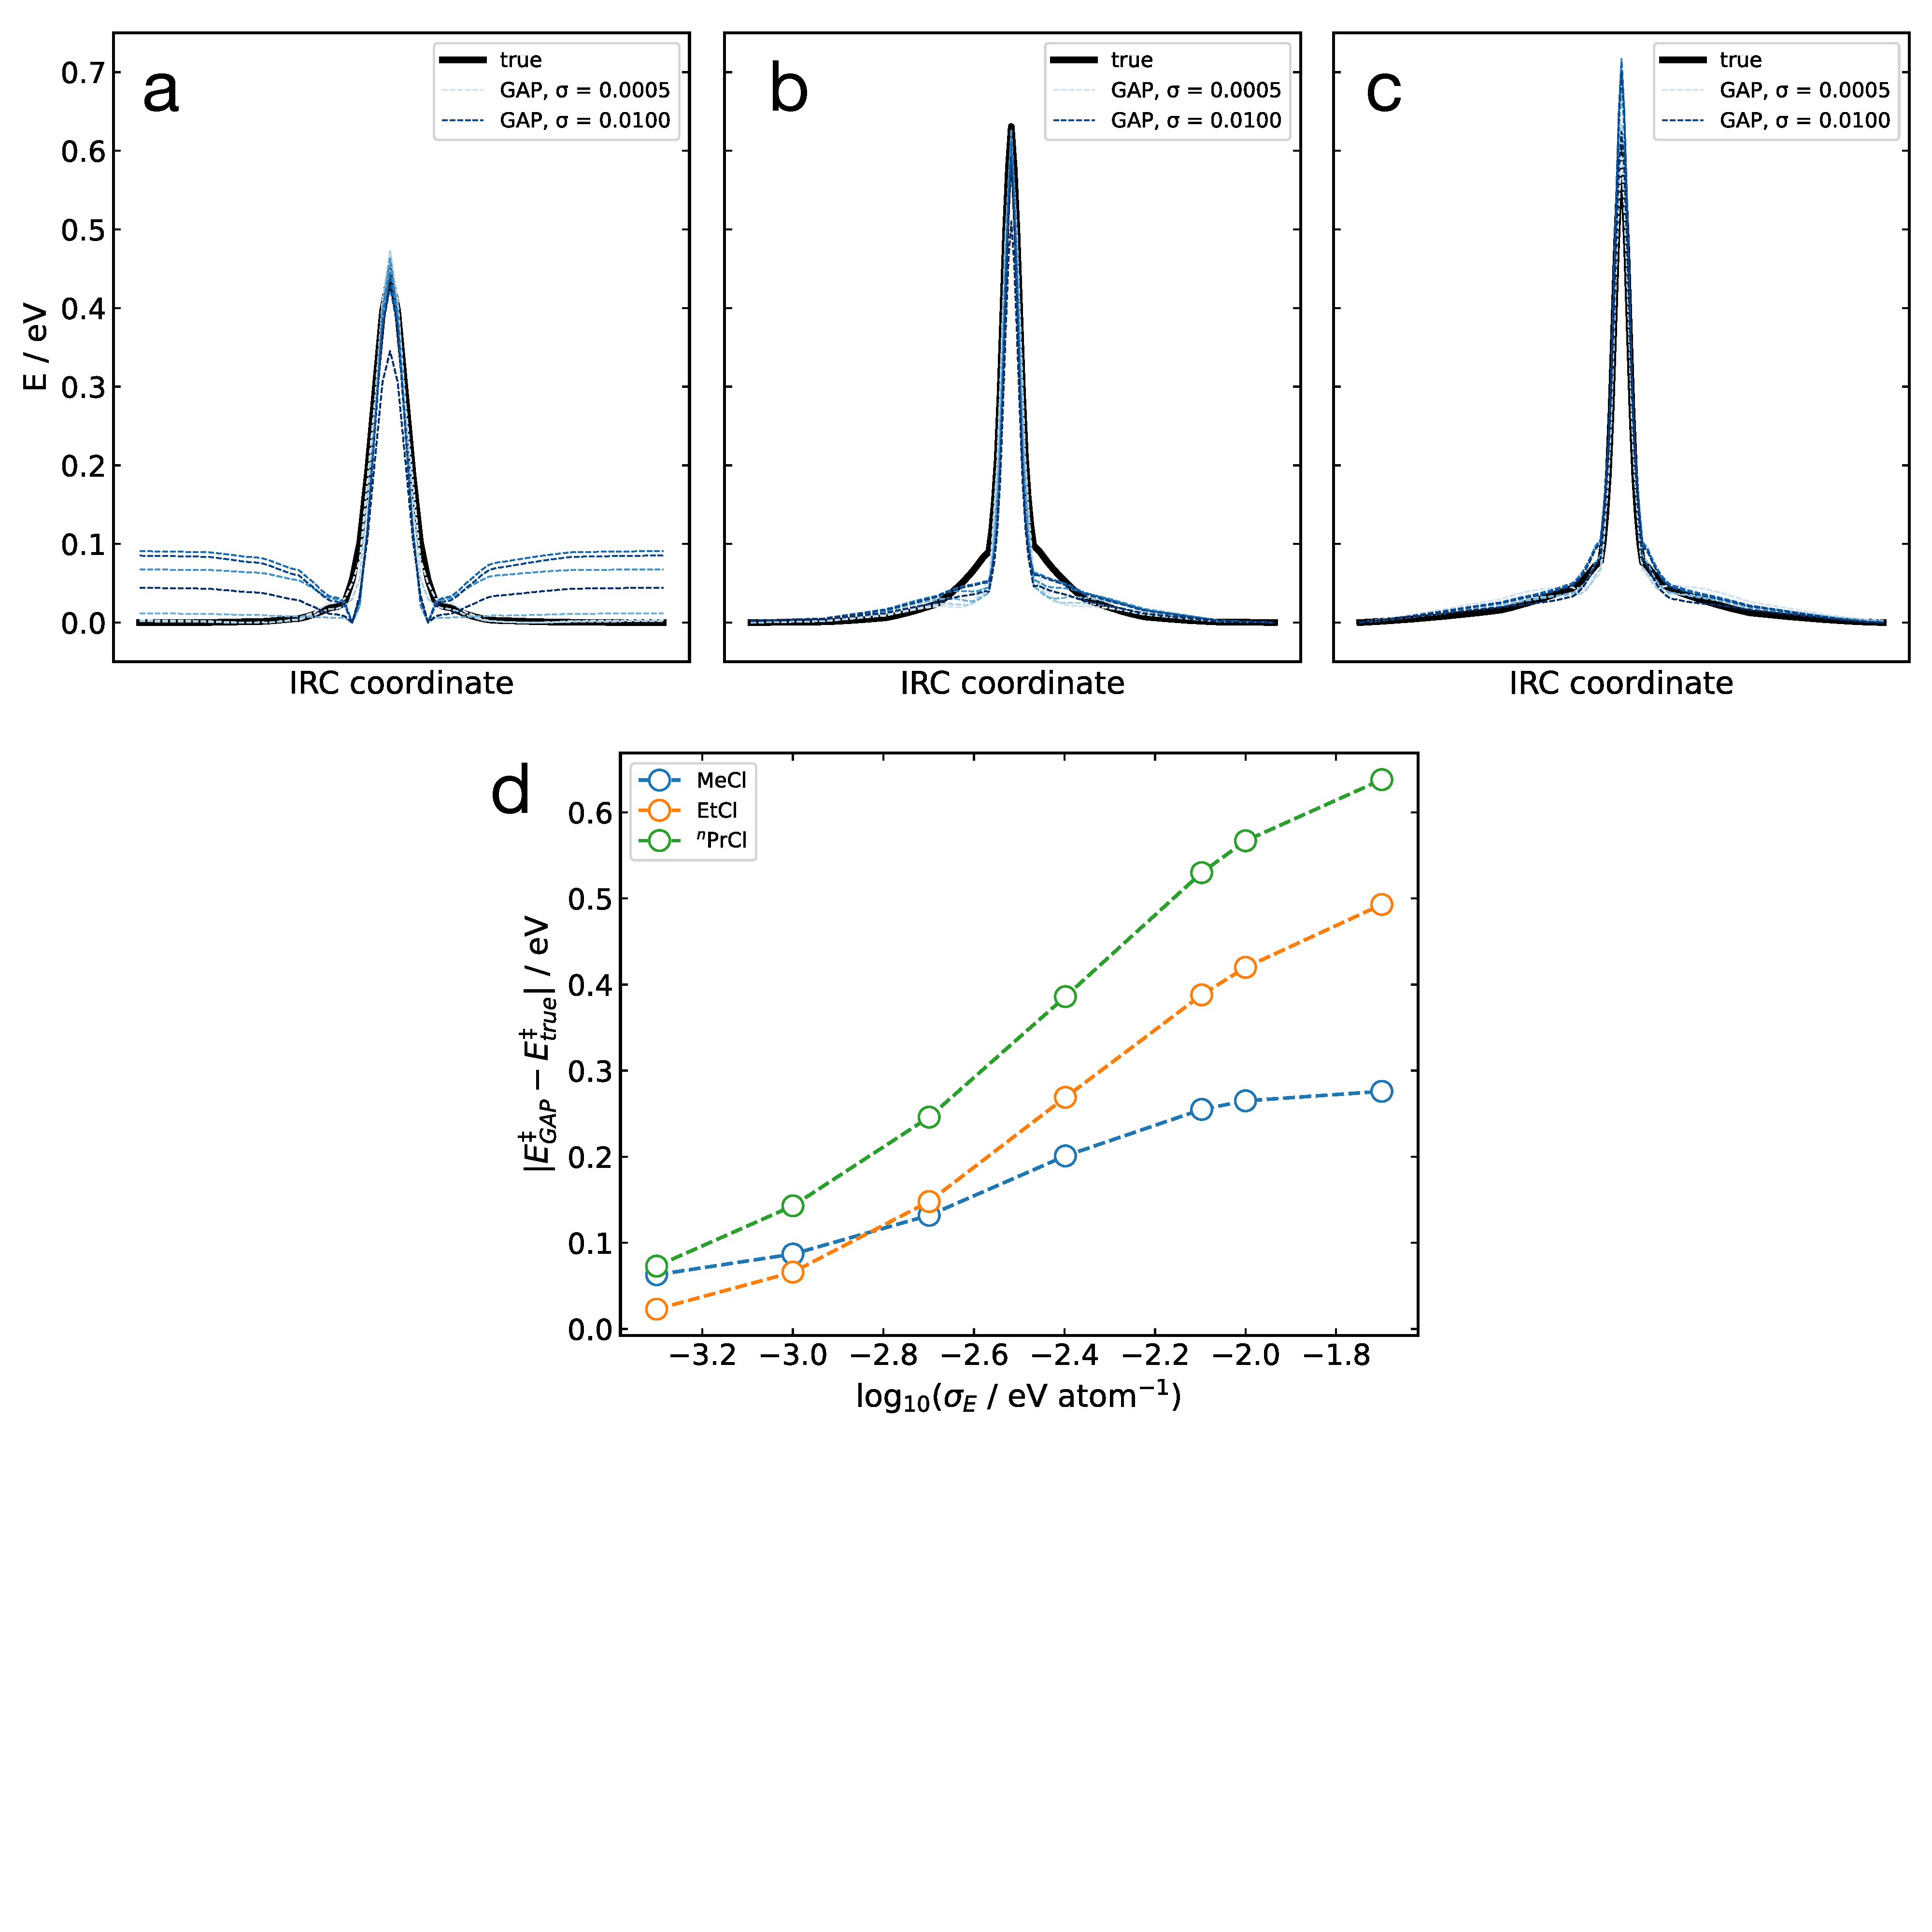
\includegraphics[width=\textwidth]{figSX19b.pdf}
	\vspace{0.0cm}
	\hrule
	\vspace{0.1cm}
	\caption{True and predicted IRCs (training data identical \figurename{ \ref{fig::SX19a}}) with GAPs trained on energies only with different $\sigma_E$ values for MeCl, EtCl, ${}^n$PrCl  (a--c respectively). Absolute error on the TS  energy for each GAP is plotted in (d).}
	\label{fig::SX19b}
\end{figure}


\clearpage
\section{Method Comparison}  \label{section:SI_mlp_comparison}

Training different MLP methods on the ethene+butadiene reaction using active learning with a selection criteria of 0.1 eV\footnote{If $|E_\text{MLP} - E_\text{true}| > 0.1$ eV then the configuration is selected in MLP-driven MD, propagated at 500 K with a 0.5 fs time step. AL is halted if 10 trajectories reach the maximum MD time of 500 fs.} affords highly accurate potentials in all cases (\figurename{ \ref{fig::SX23}}, MAD $\sim 0.04$ eV, 1 \kcal). The data requirement of the GAP (406 configurations) was significantly higher than both ACE (114) and NeQUIP (126) potentials and required significant hyper-parameter tuning (\ref{section::hyperparam_opt}). The total training time on 10 CPU cores was 7, 4 and 14 hours for GAP, ACE and NeQUIP potentials respectively, the latter also utilised an Nvidia RTX 2080 GPU.


\begin{figure}[h!]
	\centering
	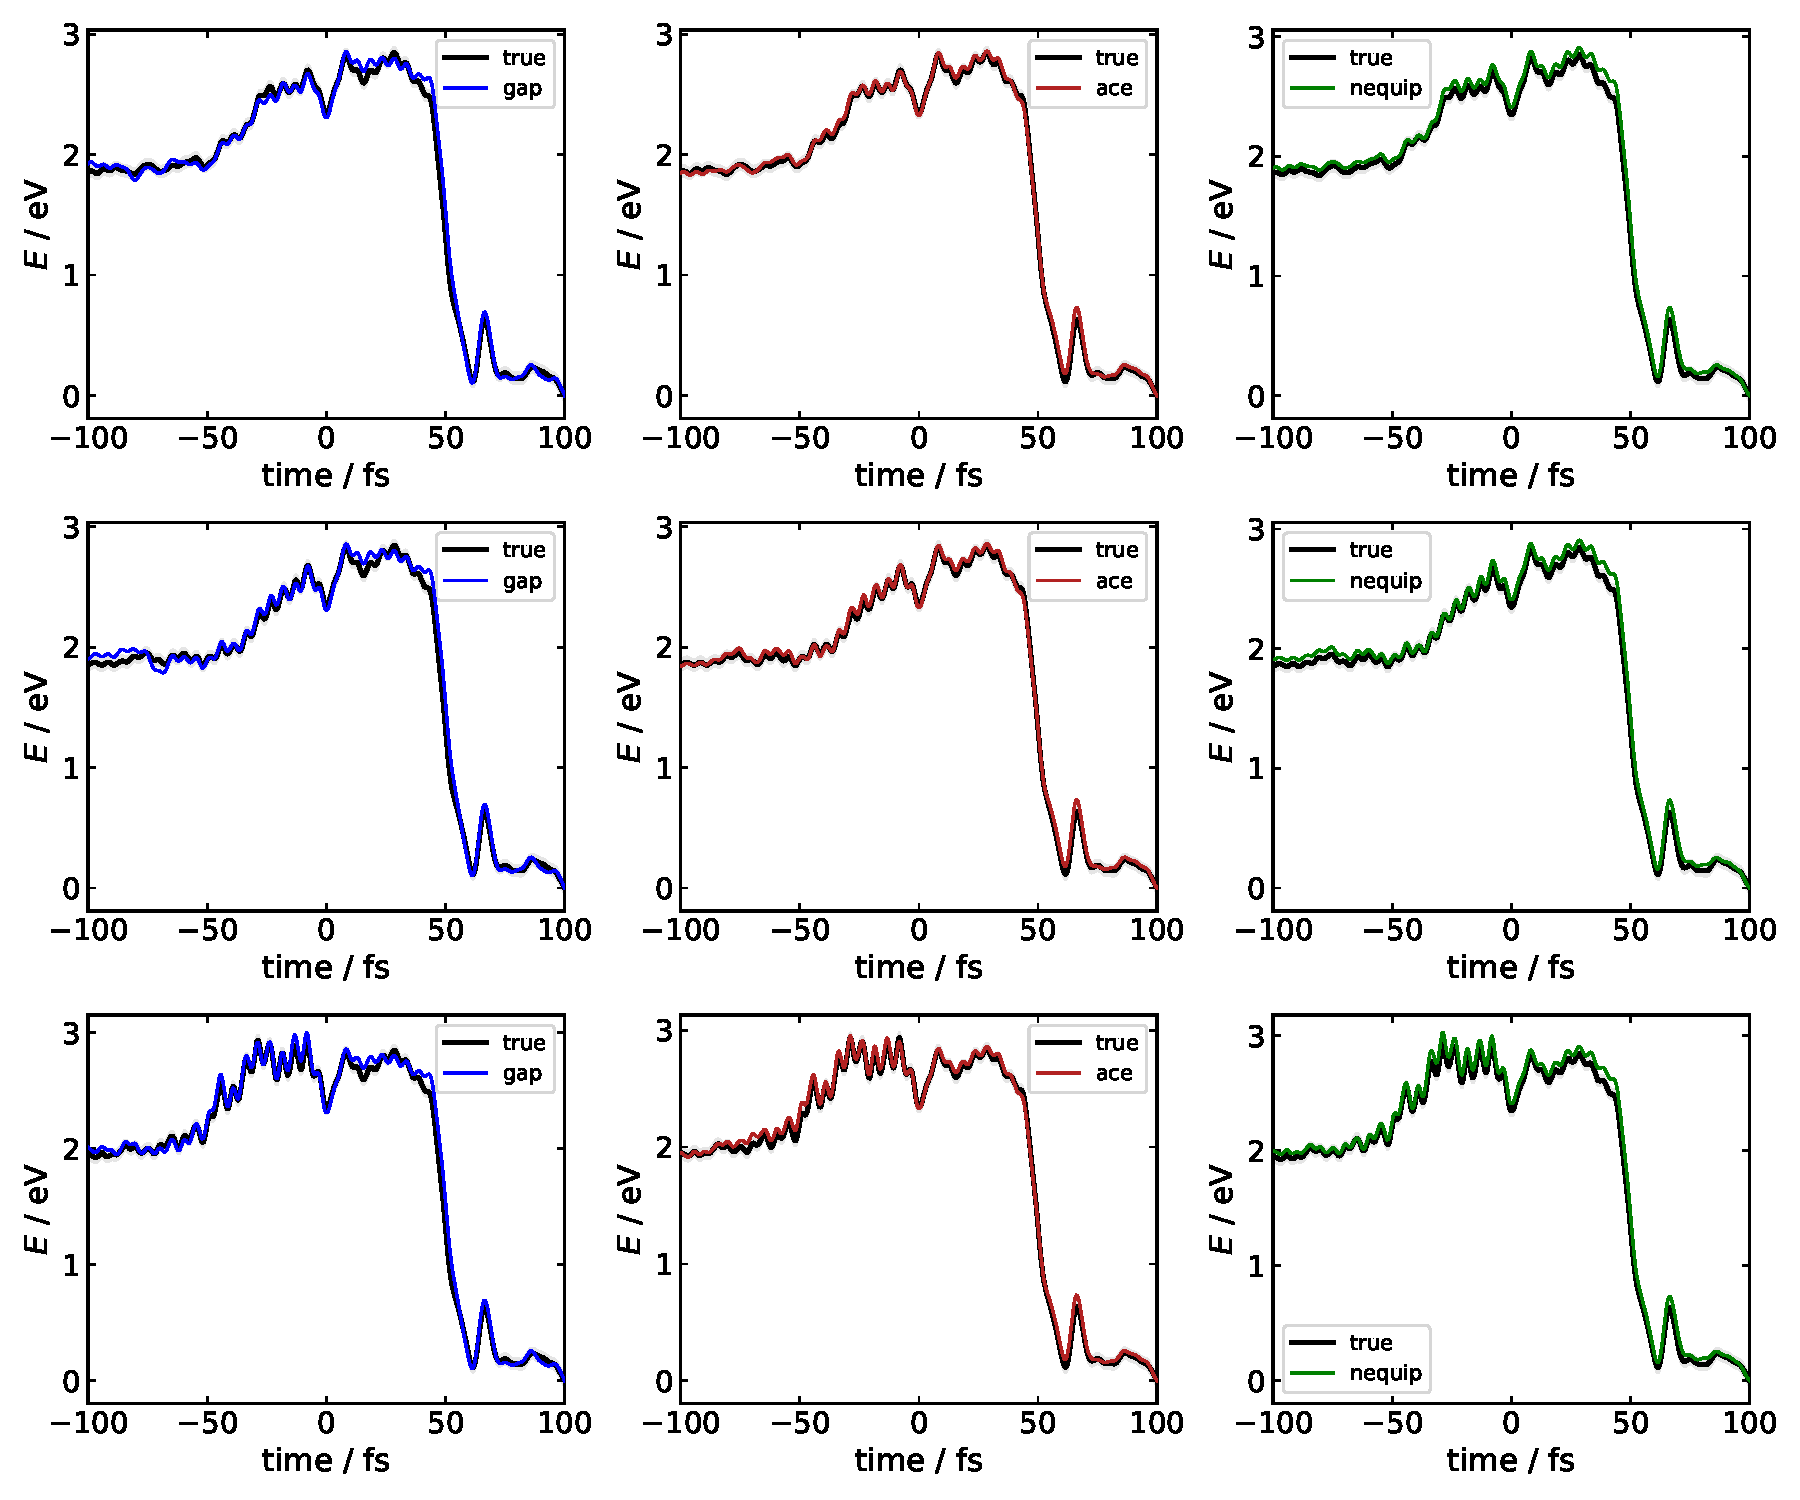
\includegraphics[width=\textwidth]{figSX23.pdf}
	\vspace{0.0cm}
	\hrule
	\vspace{0.1cm}
	\caption{Comparison of MLP methods trained using an identical AL strategy from the TS of ethene+butadiene to `ground truth' AIMD data. Both the training and AIMD used the PBE0/def2-SVP level of DFT theory. Dynamics propagated from the TS at 300 K using a Berendsen thermostat, as implemented in ORCA v. 4.2.1. Trajectories are stitched from two that proceeded forwards and backwards.}
	\label{fig::SX23}
\end{figure}


Evaluating the potentials on the intrinsic reaction coordinate again each perform comparably (\figurename{ \ref{fig::SX24}}), and all provide smooth 2D surfaces (\figurename{ \ref{fig::SX25}}). The latter is in spite of the extrapolation within high-energy regions. Interpolating the surface 


\begin{figure}[h!]
	\centering
	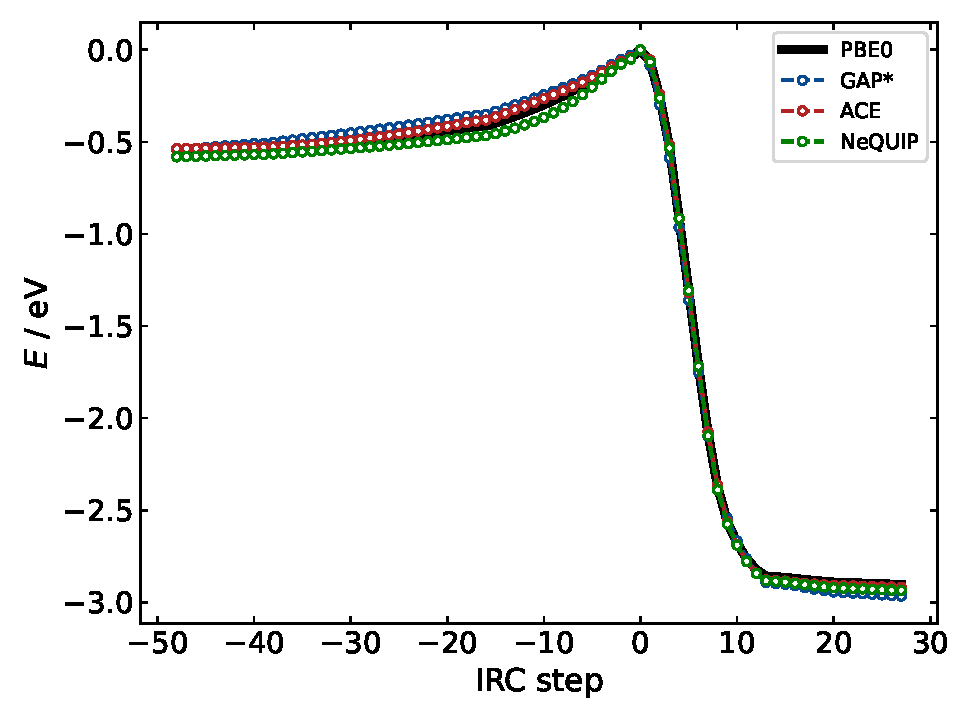
\includegraphics[height=6.4cm]{figSX24.pdf}
	\vspace{0.0cm}
	\hrule
	\vspace{0.1cm}
	\caption{Comparison of MLP methods (as \figurename{ \ref{fig::SX23}}) on the PBE0/def2-SVP intrinsic reaction coordinate (IRC).}
	\label{fig::SX24}
\end{figure}


\begin{figure}[h!]
	\centering
	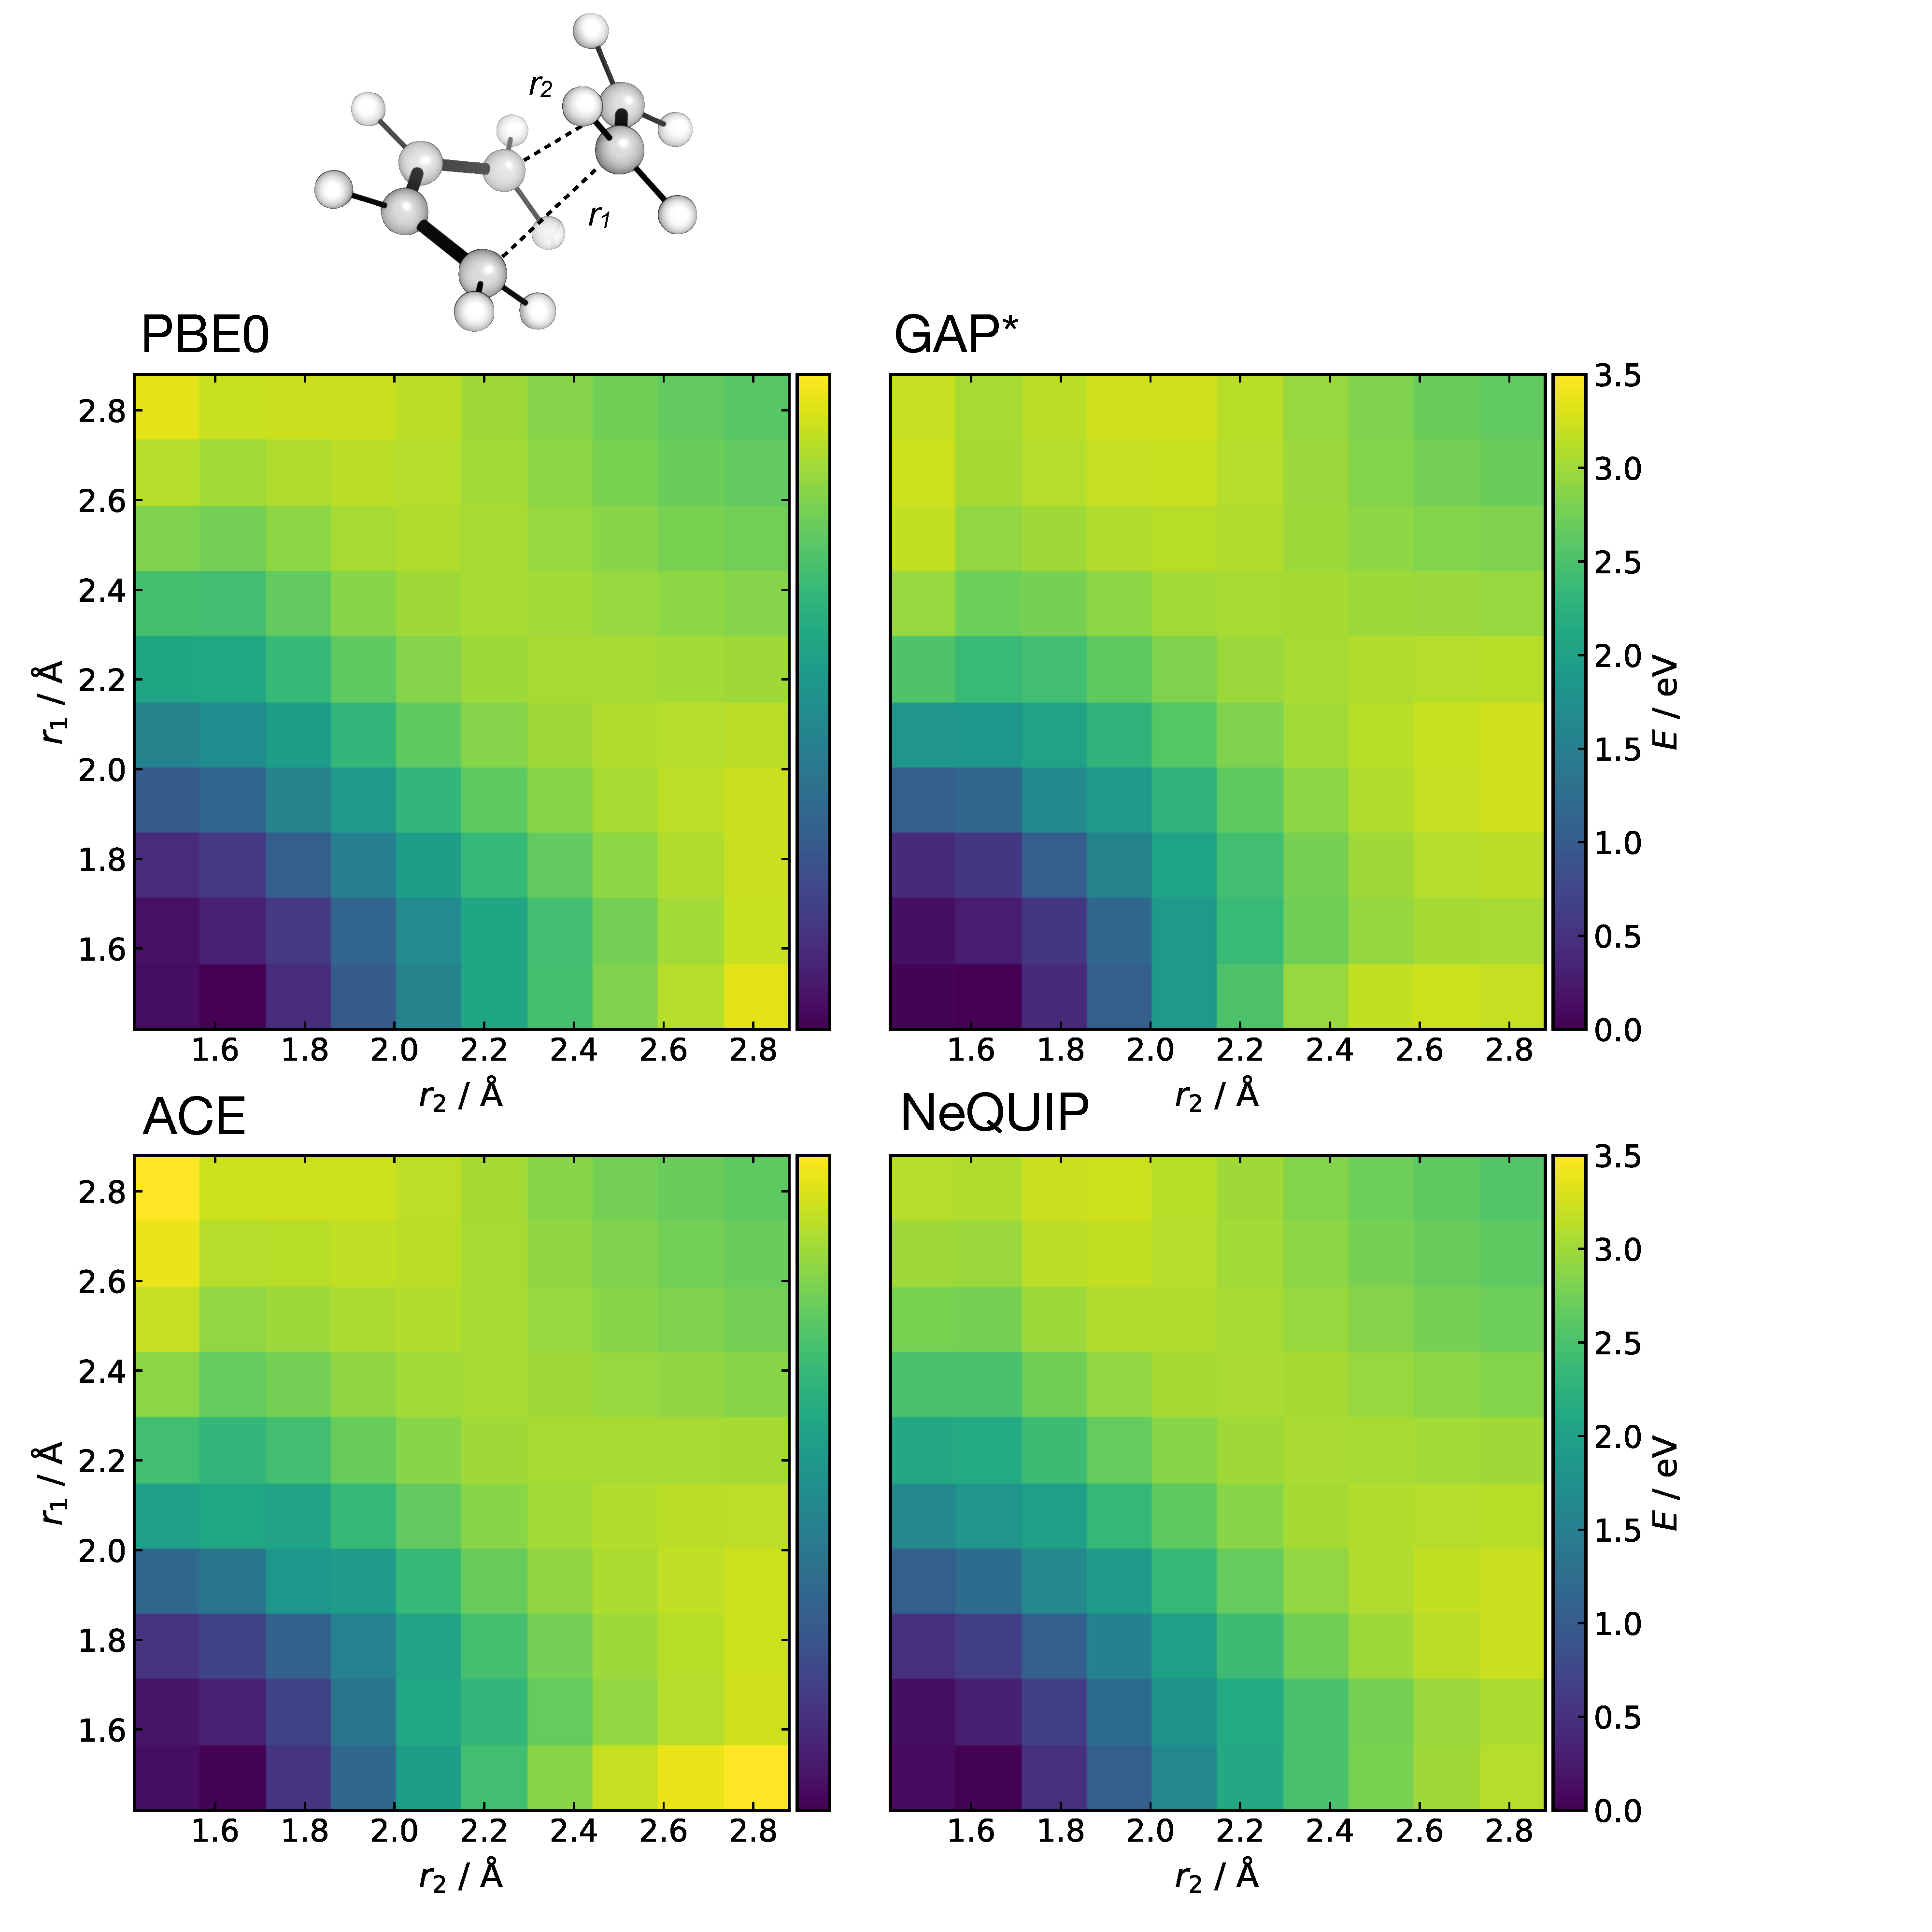
\includegraphics[width=0.8\textwidth]{figSX25.pdf}
	\vspace{0.2cm}
	\hrule
	\vspace{0.1cm}
	\caption{Comparison of MLP methods (as \figurename{ \ref{fig::SX23}}) on the PBE0/def2-SVP 2D relaxed PES.}
	\label{fig::SX25}
\end{figure}


\begin{figure}[h!]
	\centering
	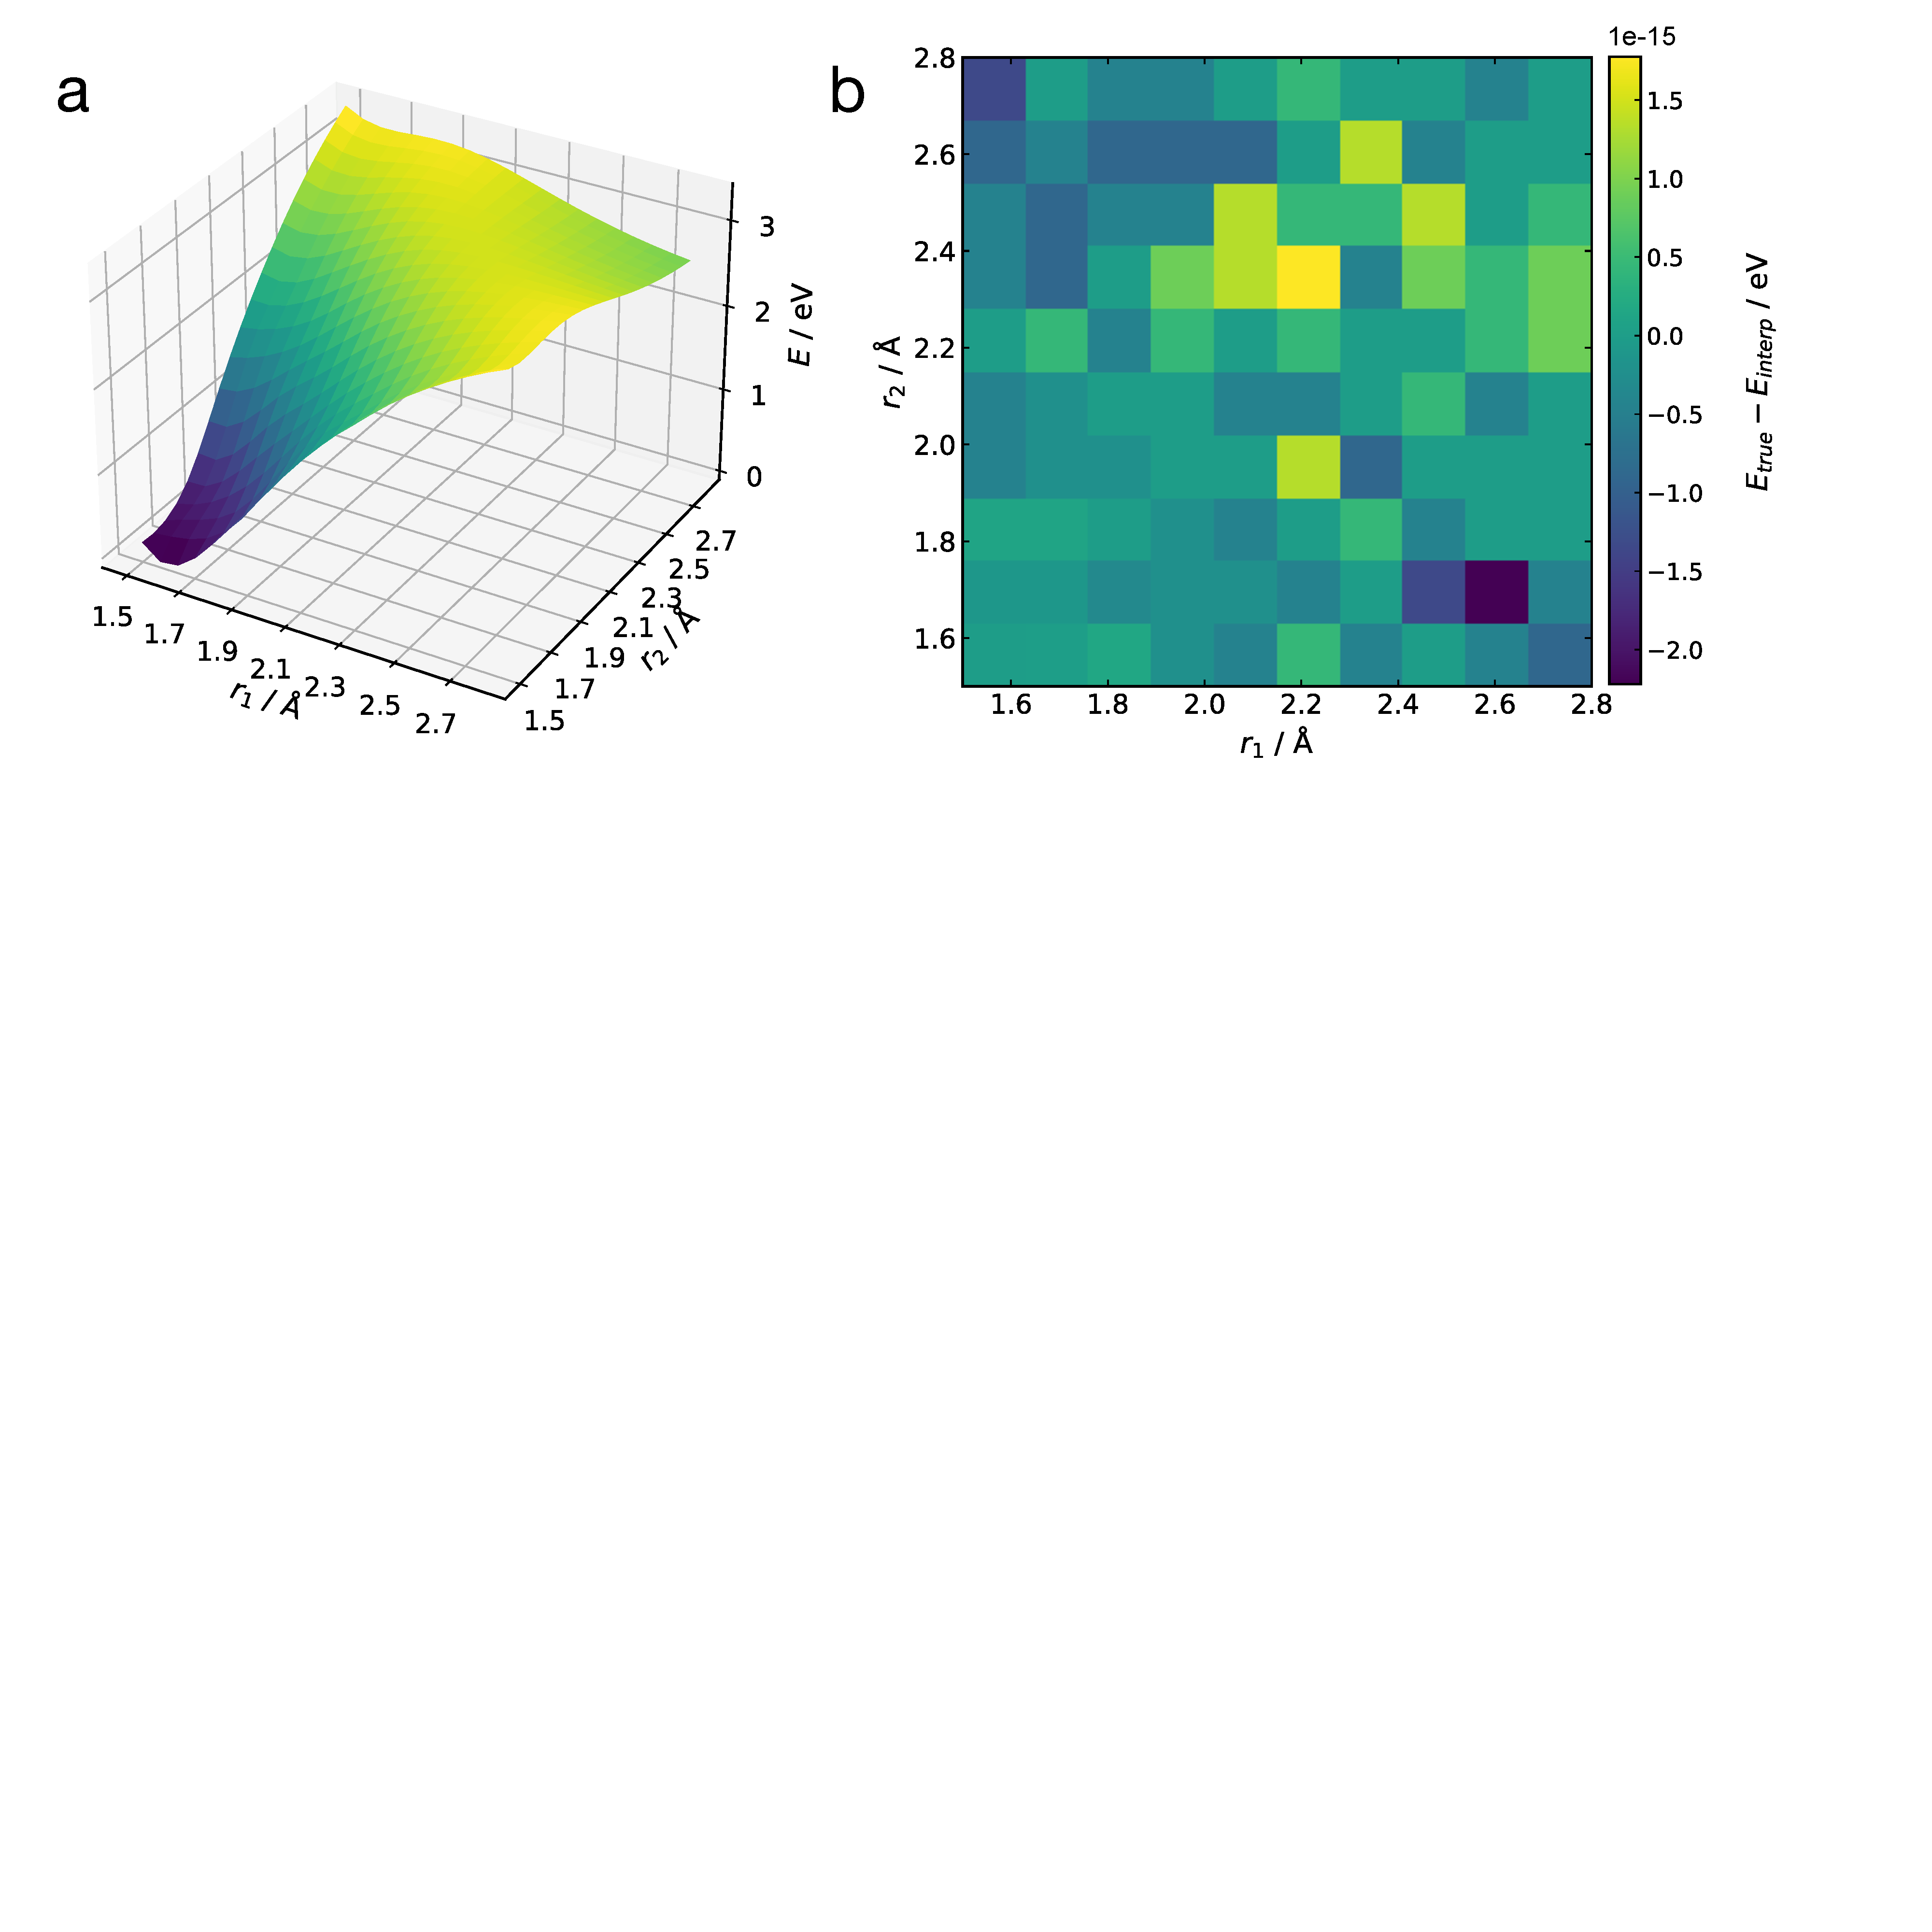
\includegraphics[height=6.4cm]{figSX26.pdf}
	\vspace{0.2cm}
	\hrule
	\vspace{0.1cm}
	\caption{(a) Interpolated 2D surface (PBE0/def2-SVP 2D relaxed PES, as \figurename{ \ref{fig::SX25}}) and (b) residuals between the interpolated and true values. Interpolation performed with \emph{RectBivariateSpline} from \emph{SciPy}.}
	\label{fig::SX26}
\end{figure}



\clearpage
\section{Active Learning Selection Strategies}  \label{section::SI_AL_strategies}


Using the predicted GP variance on a new configuration can be a highly effective selection strategy for sampling new configurations (see e.g. \figurename{ \ref{fig::SX16}}). However, when training other kinds of MLP there may be no analogue to accelerate the `diff' selection strategy.\footnote{Using $|E_\text{true} - E_\text{MLP}|$ and evaluating potentially 8 DFT evaluations with no selected configuration, for a 1 ps max time approaching the end of AL cycle.} Using a threshold on the maximum distance (`max\_dist') to any of the training set can afford a 10$\times$ speed-up in training for non-GAP MLPs where the reference evaluations dominate the execution time. Specifically, using a selection criteria defined by,

\begin{equation}
	\max(\boldsymbol{k}^*) < k_T \quad : \quad \boldsymbol{k}^* = ((\boldsymbol{p}_0 \cdot \boldsymbol{p}^*)^\zeta, \cdots)
\end{equation}

where $\boldsymbol{p}_i$ is the normalised SOAP vector for the $i$-th configuration in the training data and $\zeta$ is an positive power to sharpen differences. This is exactly the form of the kernel used in our GAPs and can provide a quantification of the similarity between one molecular configuration and another. With an appropriately chosen $k_T$, potentials can be trained efficiently (\figurename{ \ref{fig::SX28}}) despite not being correlated with the absolute energy difference (\figurename{ \ref{fig::SX27}}). 


\begin{figure}[h!]
	\centering
	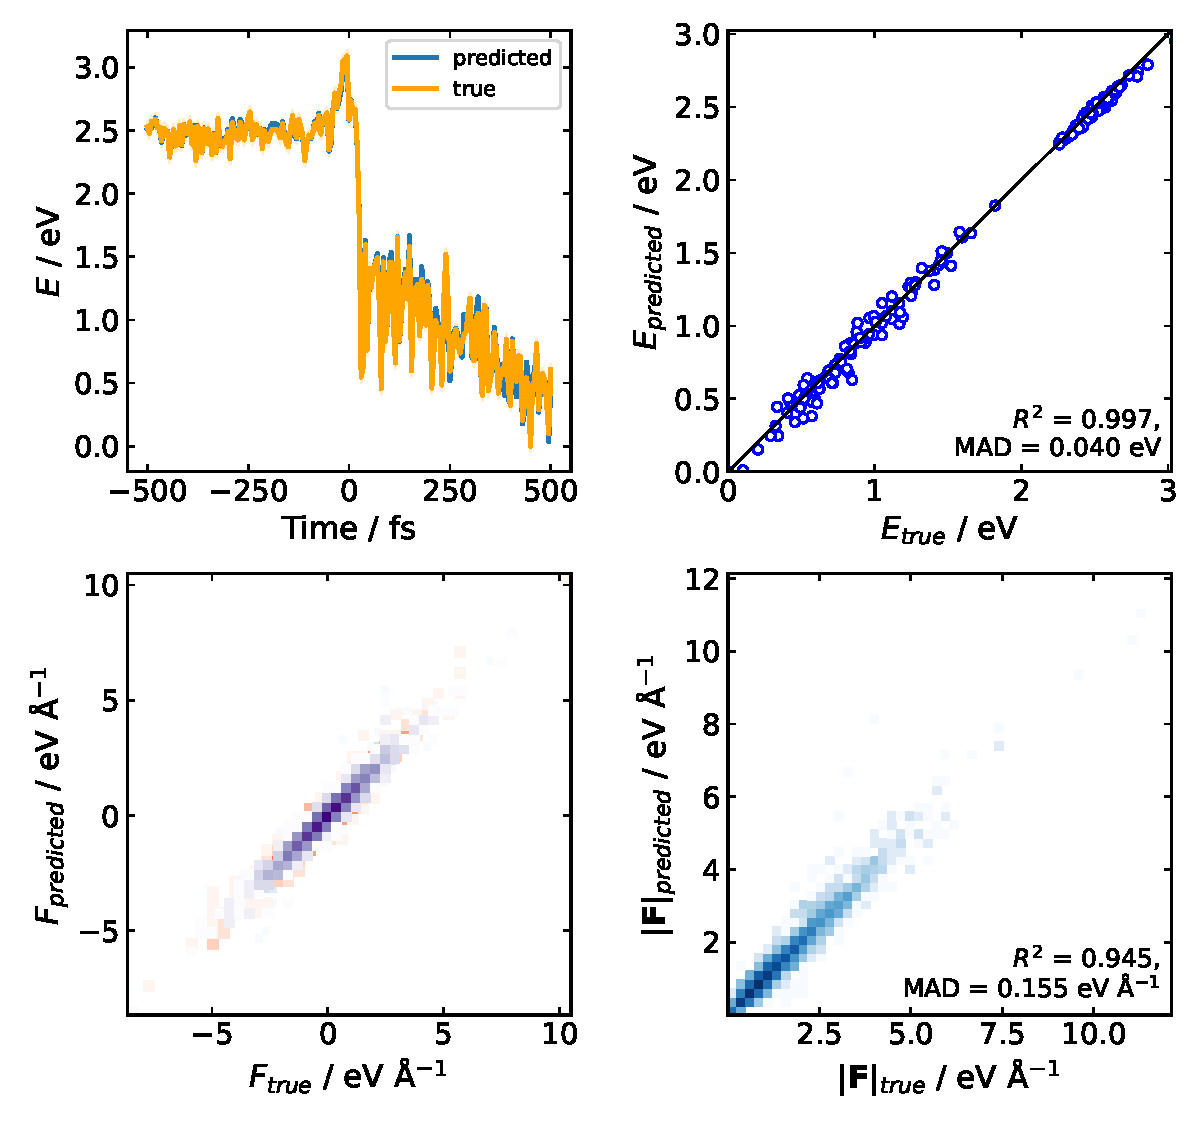
\includegraphics[height=11.2cm]{figSX28.pdf}
	\vspace{0.1cm}
	\hrule
	\vspace{0.1cm}
	\caption{Comparison of true (PBE0/def2-SVP) and predicted (ACE) energies and forces over a 500 fs ACE-propagated trajectory from the TS (300 K, $\delta t$ = 0.5 fs). ACE potential trained using a `max\_dist' AL strategy ($k_T = 0.999$), which generated 104 configurations.}
	\label{fig::SX28}
\end{figure}



\begin{figure}[h!]
	\centering
	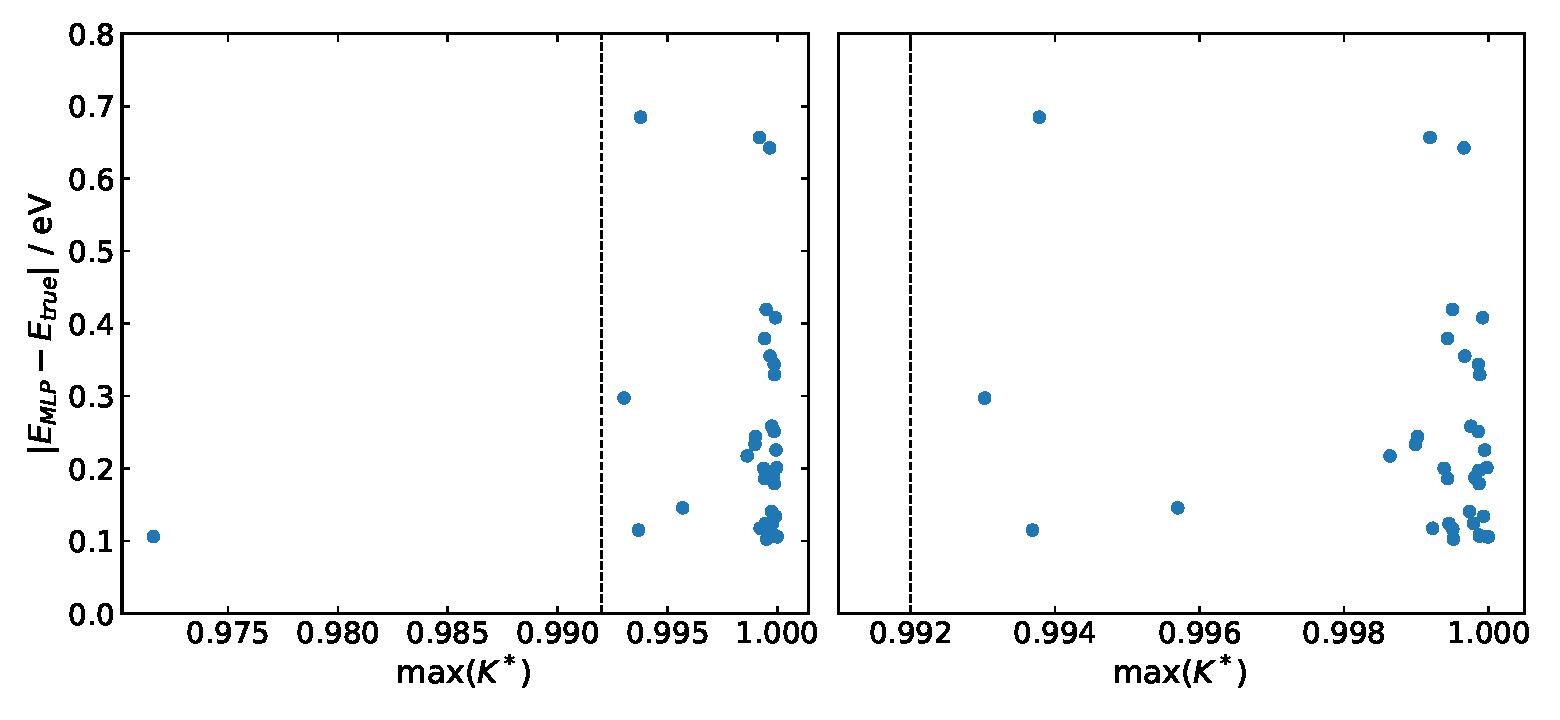
\includegraphics[height=6.4cm]{figSX27.pdf}
	\vspace{0.1cm}
	\hrule
	\vspace{0.1cm}
	\caption{Correlation of maximum SOAP kernel vector values with true differences, showing a no expected negative correlation. Frames selected over a 5000 K active learning trajectory of methane, using GAP MLP.}
	\label{fig::SX27}
\end{figure}



Using this strategy it is essential to backtrack until $\max(\boldsymbol{k}^*)$ is not \emph{too} small, to prevent high-energy structures (or SCF convergence failures) making their way into the training data. We found an upper threshold of $(k_T)^2$ to be sufficient without much tuning and $\zeta = 8$ to be optimal.


Direct use of this strategy to train a ACE potential for the DA/cope reactions between tropone and cycloheptatriene did afford a reasonable potential, but during AL training there was no sampling of one of the DA products.


\newpage
\section{Method Effects on Product Distributions}  \label{section::SI_method_effects_R3}


\begin{figure}[h!]
	\centering
	\vspace{0.4cm}
	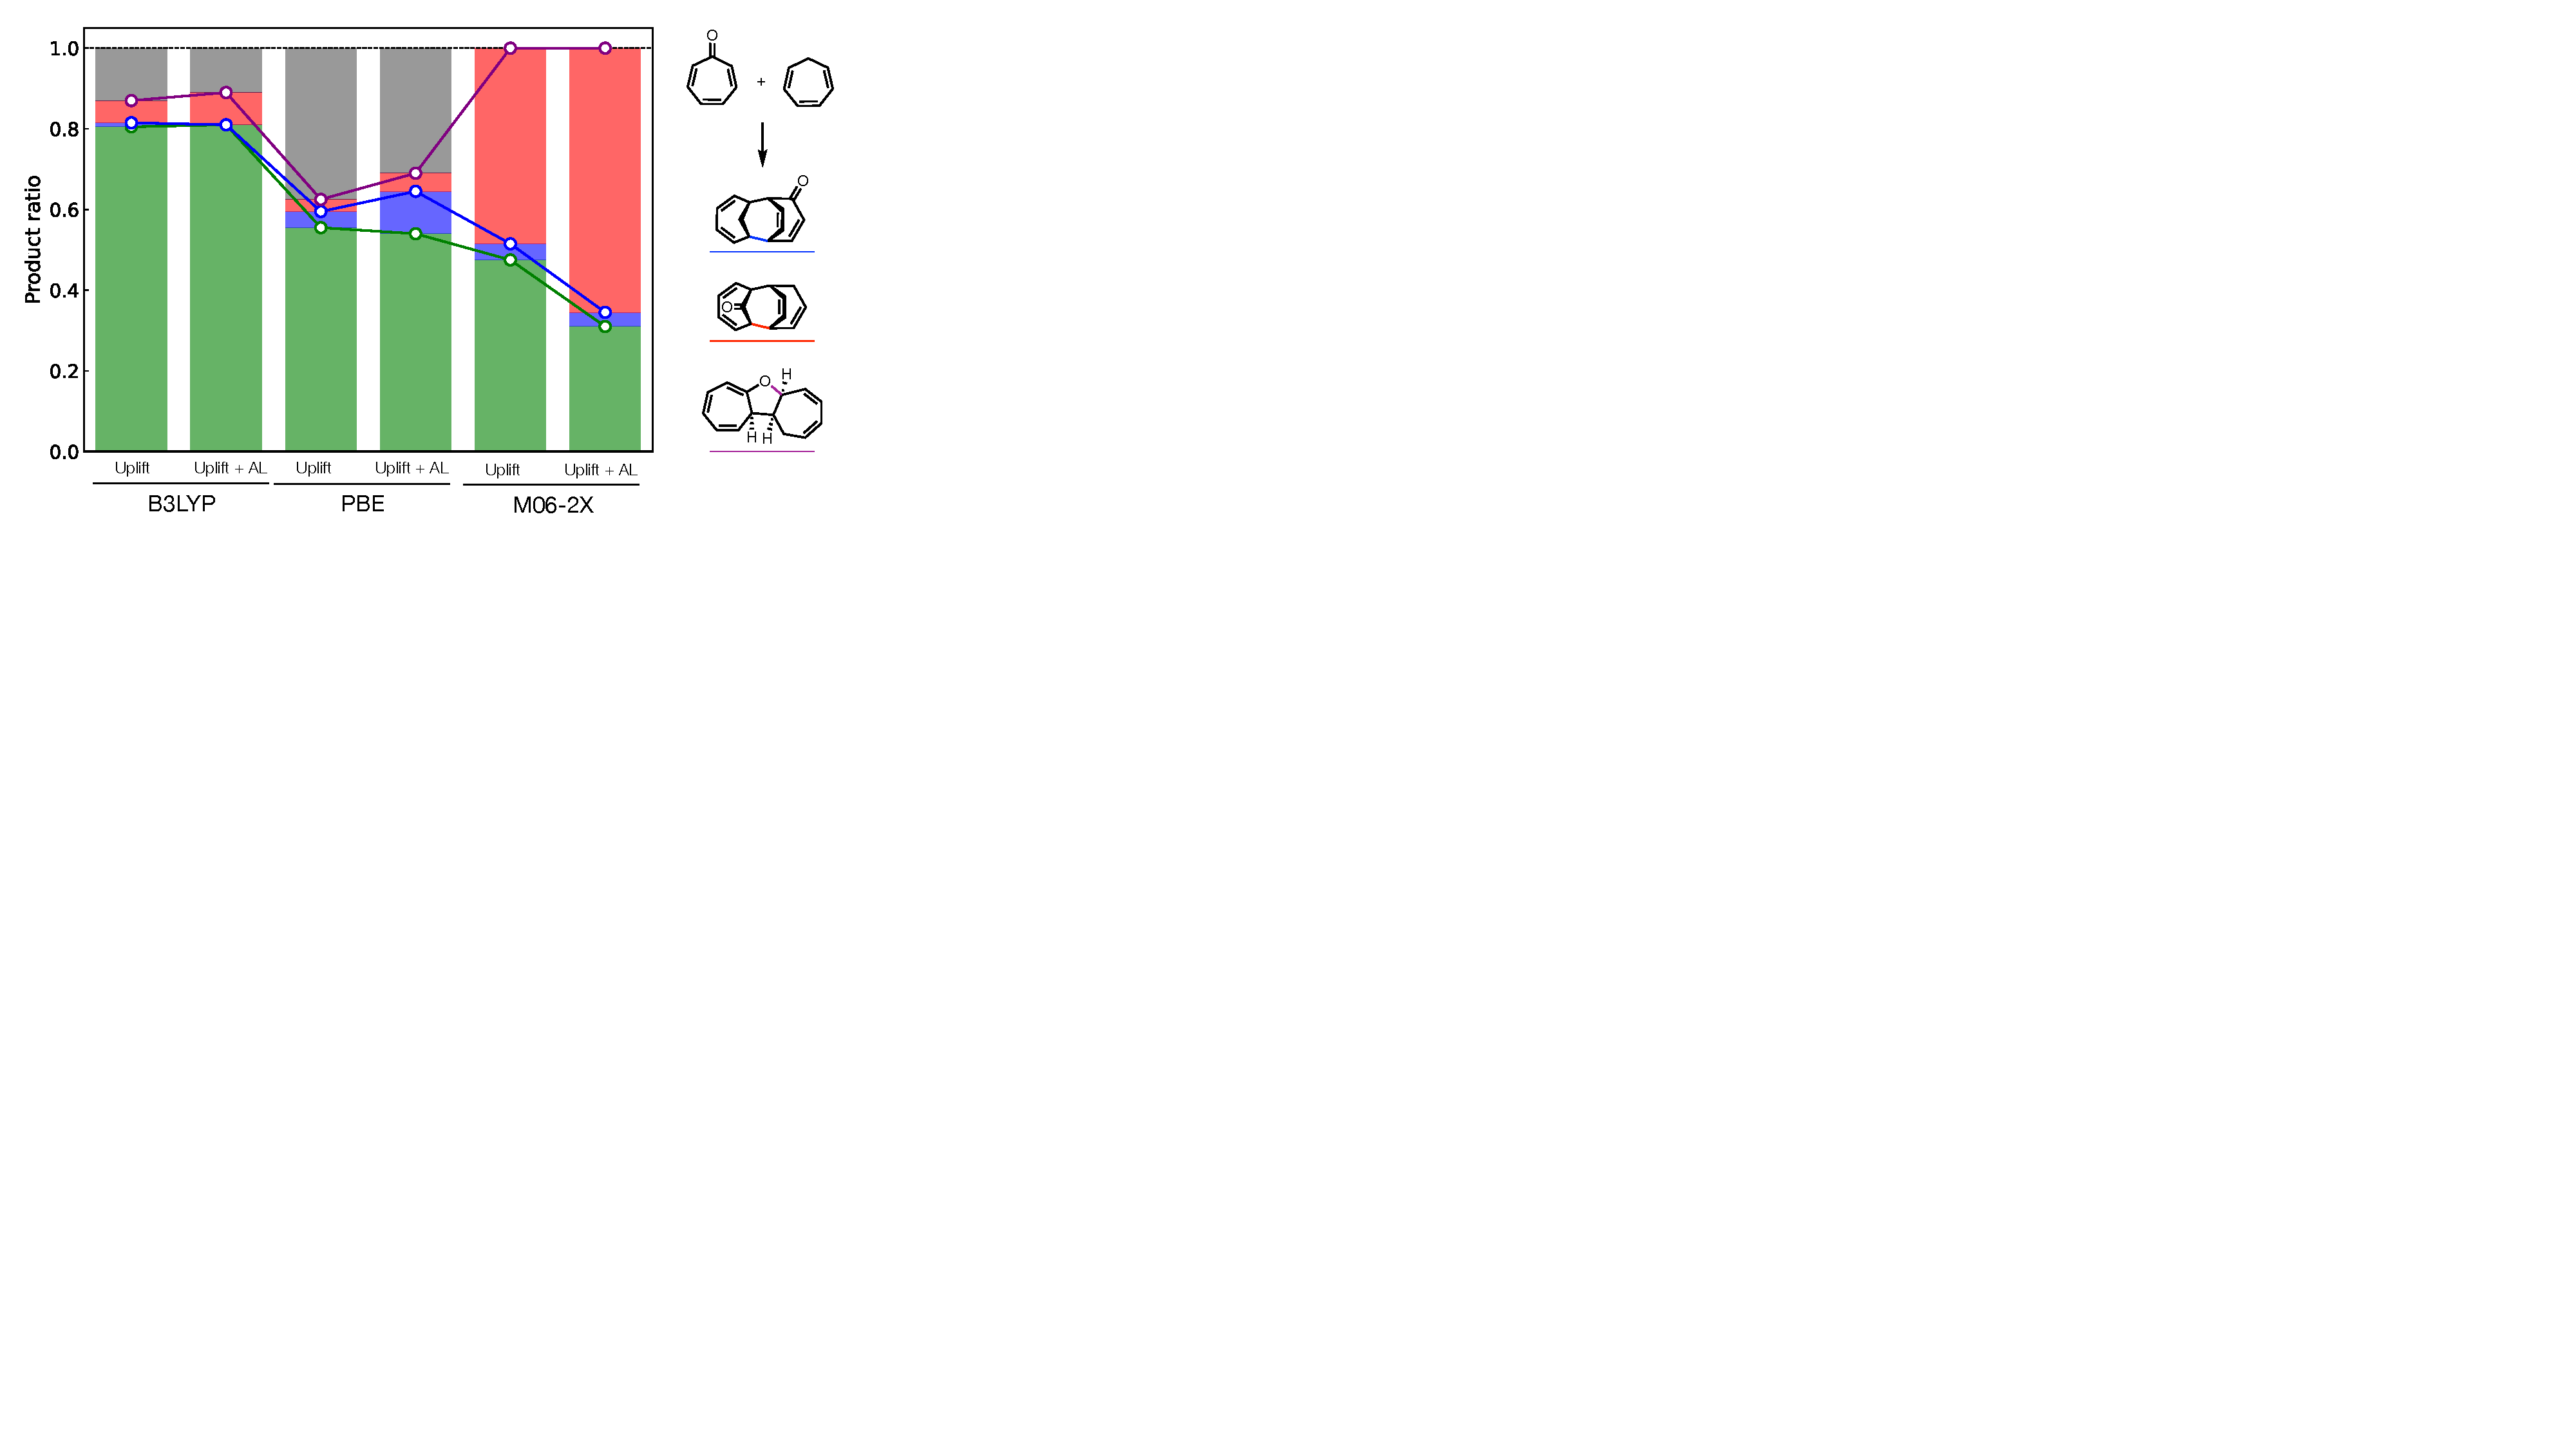
\includegraphics[height=6.4cm]{figSX31.pdf}
	\vspace{0.1cm}
	\hrule
	\vspace{0.1cm}
	\caption{Product distribution generated from 200 classical NVE trajectories propagated from 'the' TS at B3LYP, PBE and M06-2X levels of theory (def2-SVP) using initial velocities for 300 K for 1 ps using a 0.5 fs time step. Colours correspond to the products, with green the reactant state and grey no defined state being formed in 1 ps. Uplifted corresponds to single point energy and force evaluations on ACE AL configurations (PBE0/def2-SVP) then retraining the ACE potential. Uplift+AL uses PBE0 configurations reevaluated plus 5 iterations of active learning at 500 K from the appropriate TS.
}
	\label{fig::SX31}
\end{figure}

\clearpage
\section{Tropone + cycloheptatriene} \label{section::SI_accuracy_R3}

Accuracy of the ACE potential trained for the reaction between tropone + cycloheptatriene is outlined in \figurename{ \ref{fig::SX33}}, with \tacc $>1$ ps from both the ambimodal and Cope TSs (see ref. \cite{Young2021gap} for a definition of \tacc).

\begin{figure}[h!]
	\centering
	\vspace{0.4cm}
	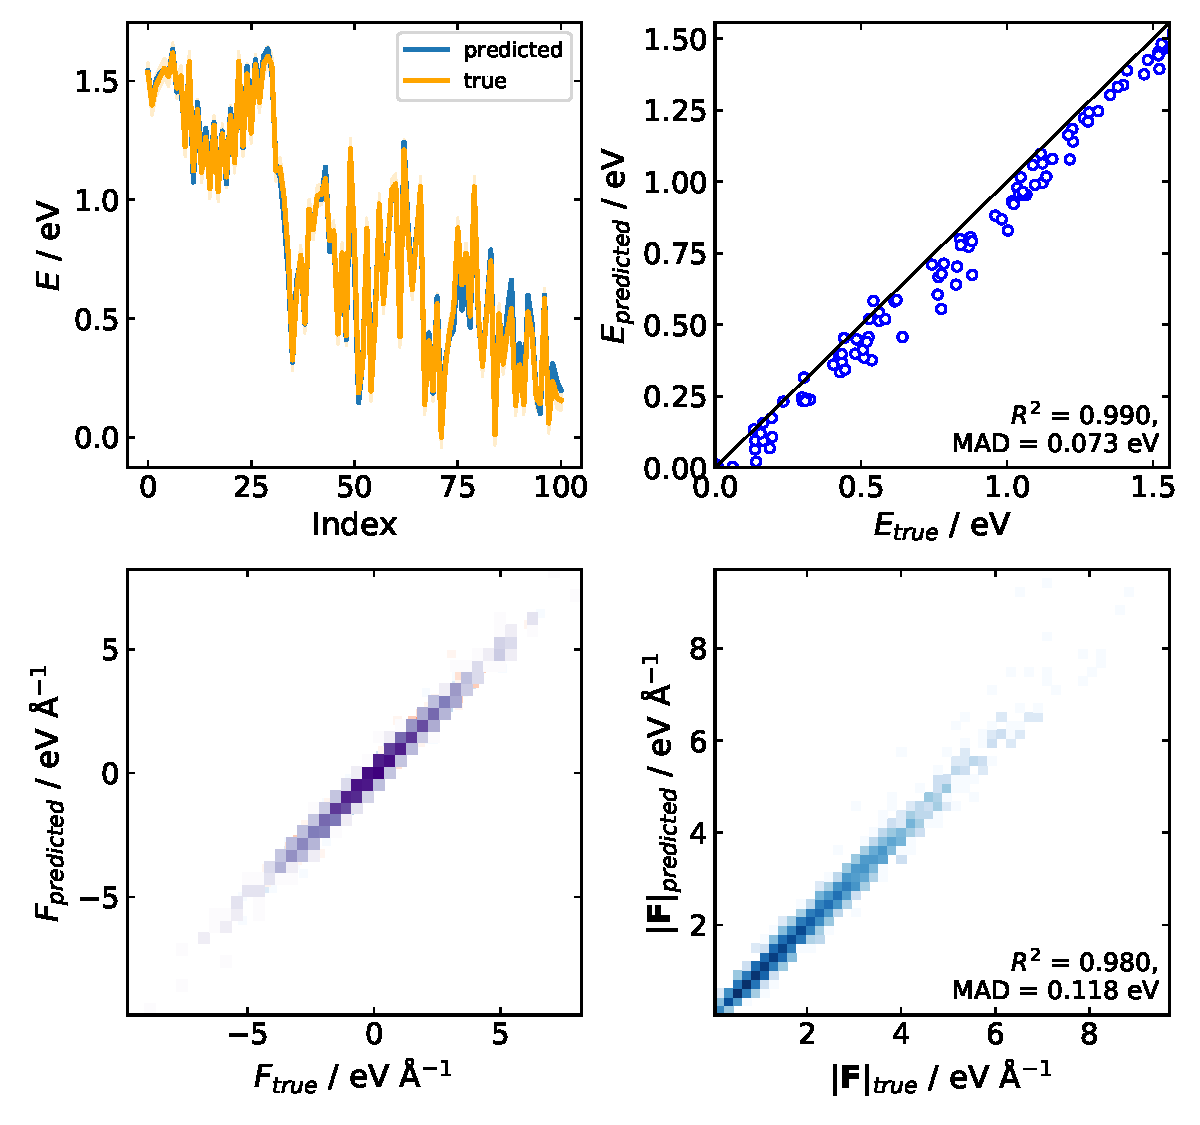
\includegraphics[height=11.2cm]{figSX33.pdf}
	\vspace{0.1cm}
	\hrule
	\vspace{0.1cm}
	\caption{Accuracy of an ACE potential on ACE-MD dynamics from the ambimodal TS between tropone + cycloheptatriene. AL initiated from two TSs at 500 K for a maximum time of 1 ps per AL iteration. Converged training data contains 453 configurations. PBE0/def2-SVP level of theory.}
	\label{fig::SX33}
\end{figure}



\clearpage 
\section{Methyl vinyl ketone + cyclopentadiene} \label{section::SI_umbrella_R2}


\begin{figure}[h!]
	\centering
	\vspace{0.4cm}
	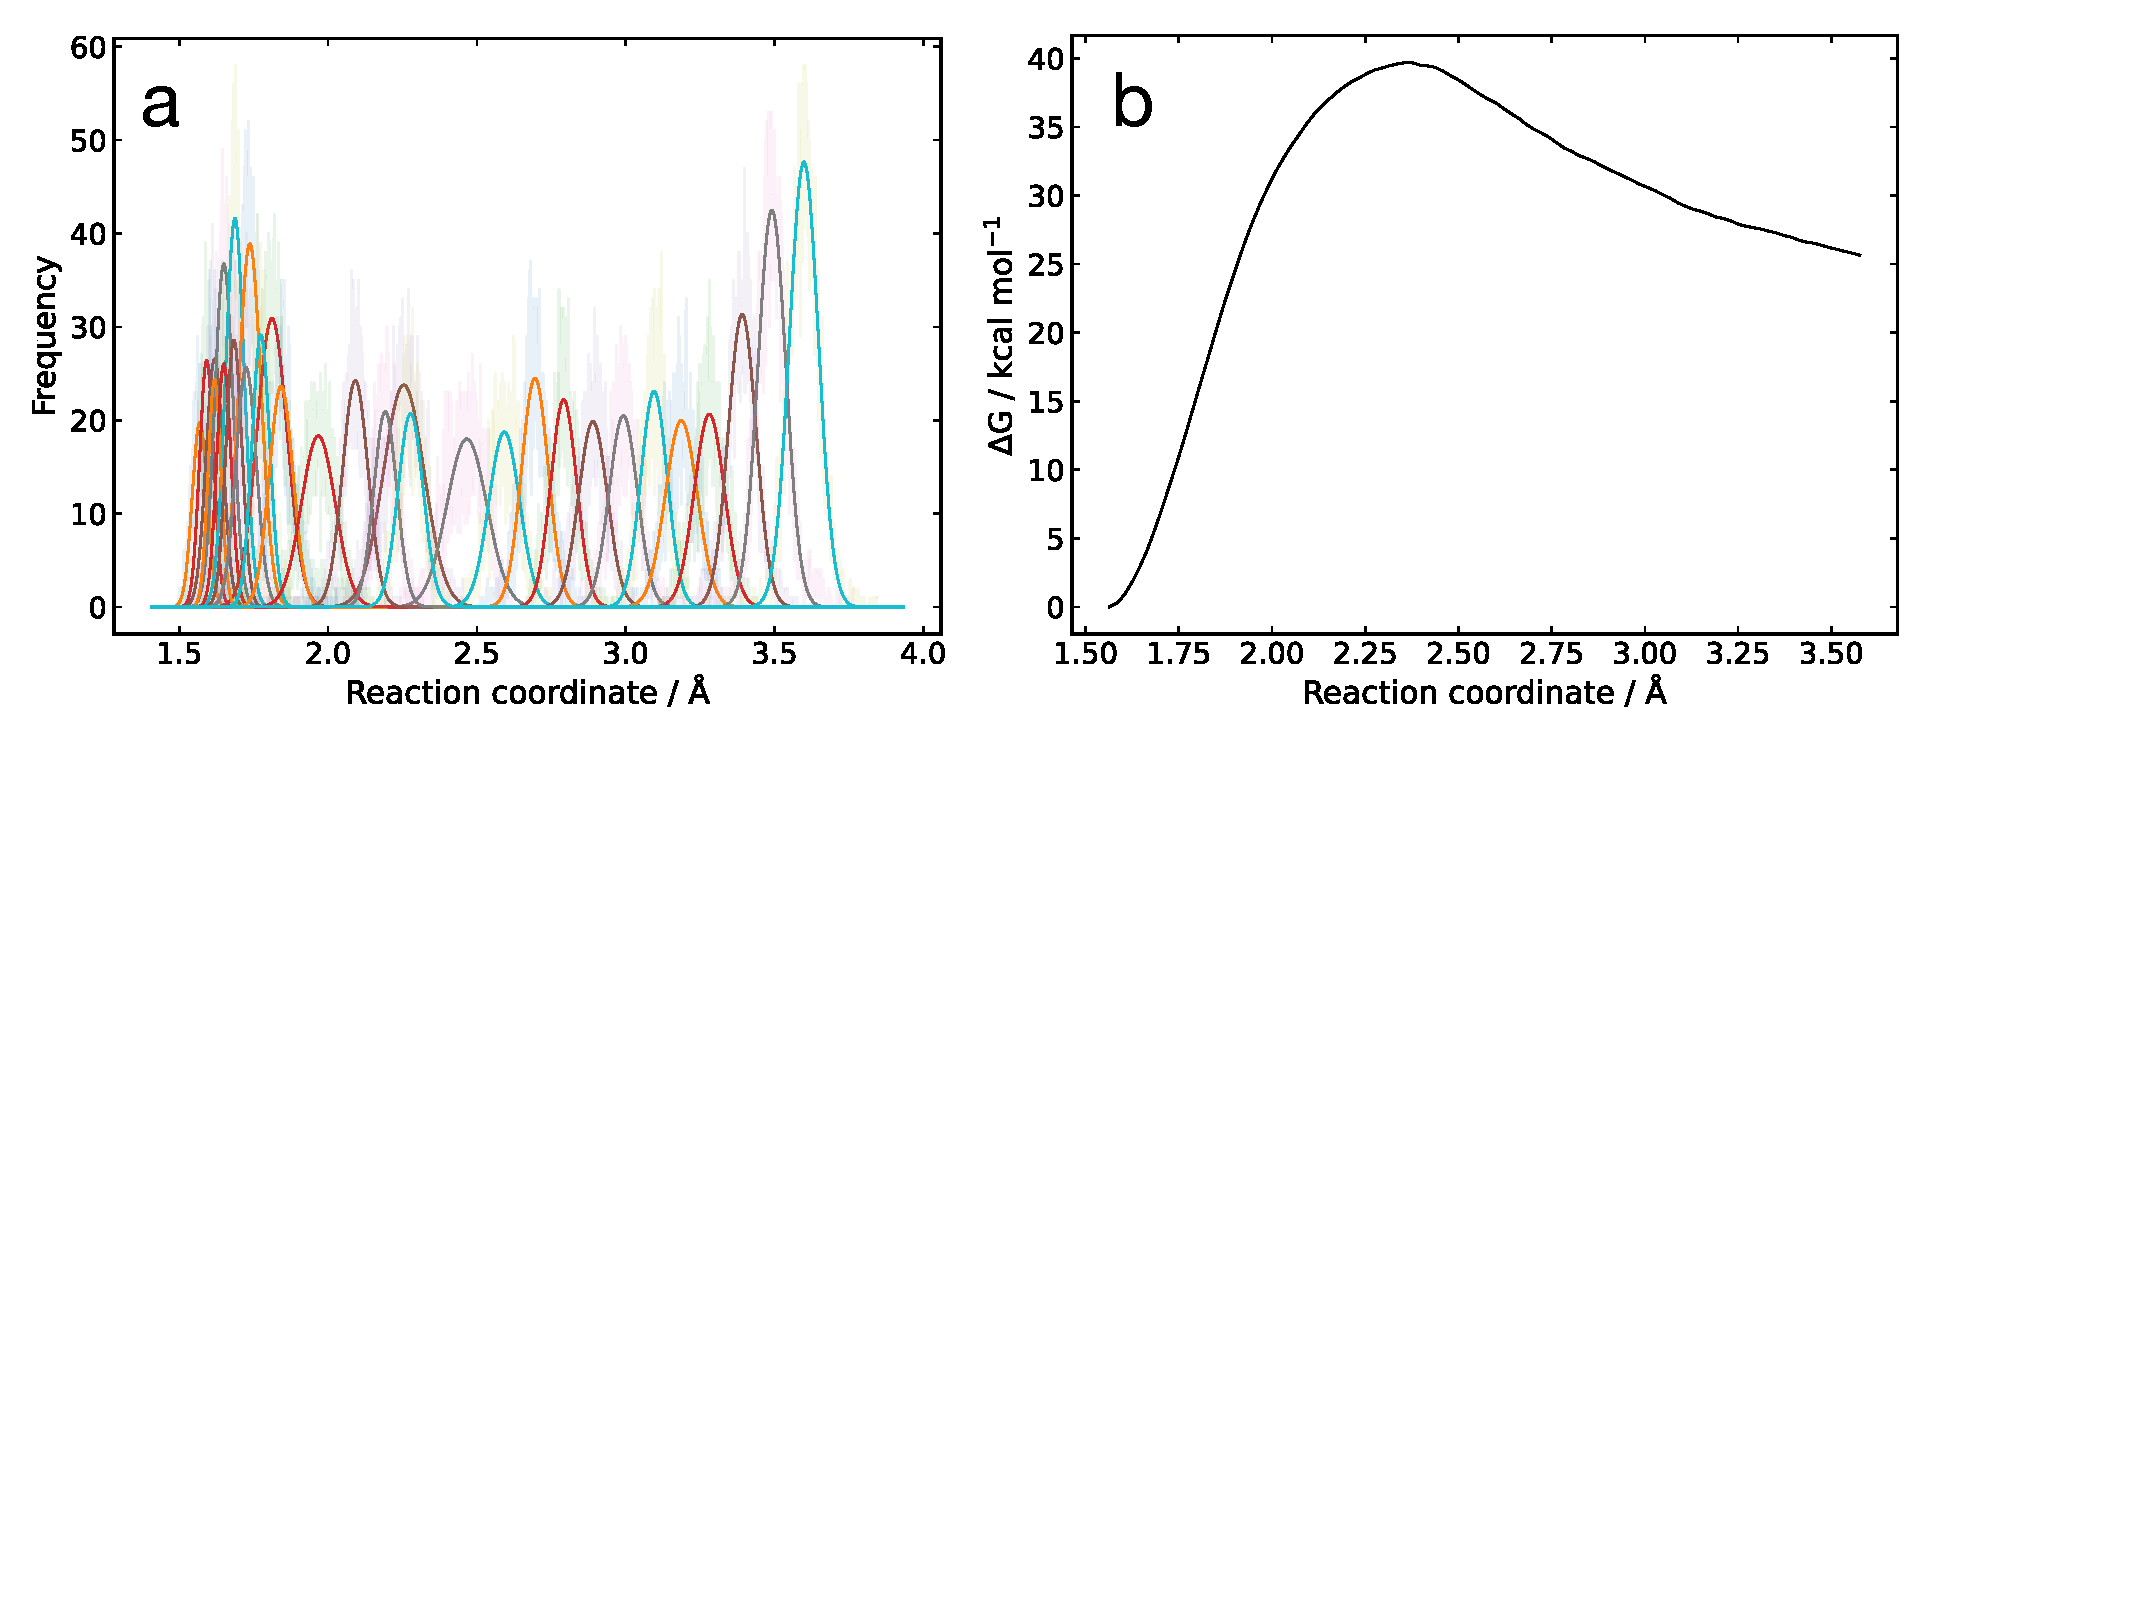
\includegraphics[height=6.2cm]{figSX34.pdf}
	\vspace{0.1cm}
	\hrule
	\vspace{0.1cm}
	\caption{Example of an umbrella sampling simulation. 300 K, 0.5 fs time step, 10 ps per window. 20 windows equally spaced in [1.564, 3.5765] \AA with $k = 10$ eV \AA${}^{-1}$ and 10 equally spaced over [1.7, 2.3] \AA with $k = 20$ eV \AA${}^{-1}$. (a) Histogrammed reaction coordinate, defined by the average of the two forming bonds, for each umbrella containing a harmonic bias. (b) Free energy obtained from weighted histogram analysis (WHAM) unbiasing of the simulation; approximately equal to the potential of mean force (PMF).}
	\label{fig::SX34}
\end{figure}



\clearpage 
\section{Acetylene + cyclopentadiene} \label{section::SI_R4}

With a view to obtain an accurate ACE potential capable of direct comparison to experimental enthalpy and entropies of activation we selected the reaction between cyclopentadiene and acetylene, for which high-quality experimental data is available. Re-analysis of the data in ref. \cite{Walsh1975} with an Eyring analysis afforded the experimental activation parameters (\figurename{ \ref{fig::SX35}}).


\begin{figure}[h!]
	\centering
	\vspace{0.4cm}
	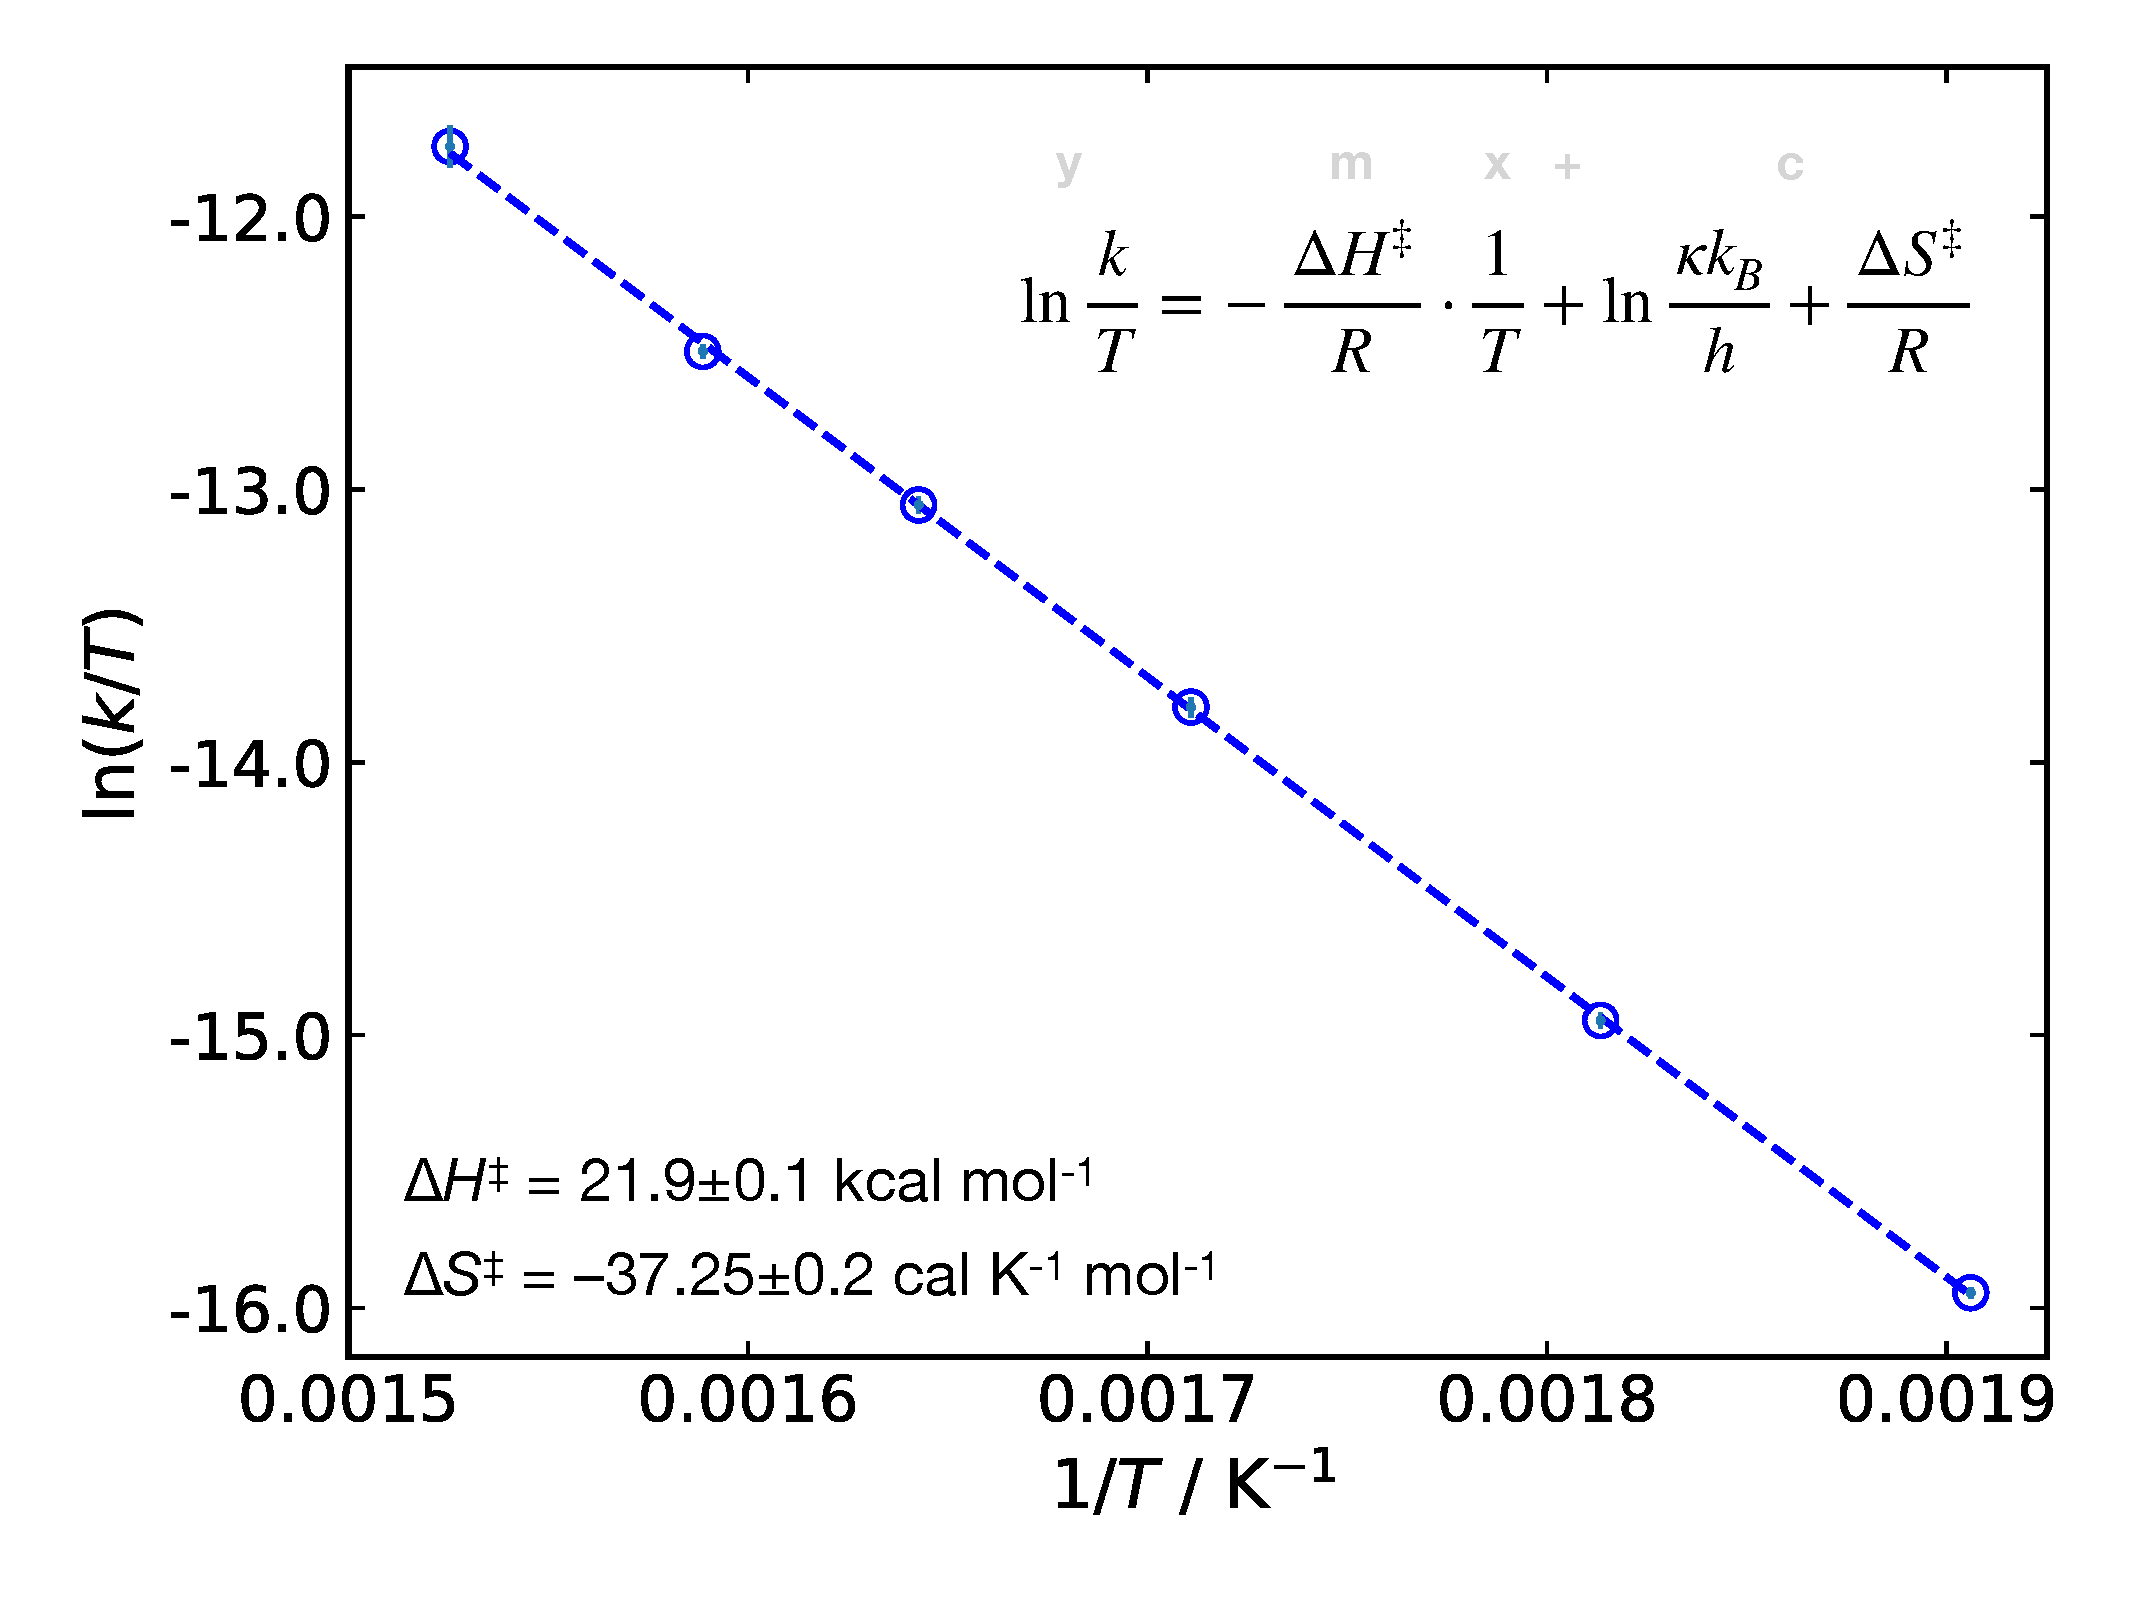
\includegraphics[height=6.4cm]{figSX35.pdf}
	\vspace{0.1cm}
	\hrule
	\vspace{0.1cm}
	\caption{Eyring analysis of the rate data in ref. \cite{Walsh1975}. Rate coefficients in units of atm$^{-1}$ s$^{-1}$ thus $\ln(k/T)$ includes an implicit factor of (atm K s). Linear fit performed with \emph{scipy.stats.linregress} (v. 1.7.1) with the associated errors in derived quantities quoted as the standard errors.}
	\label{fig::SX35}
\end{figure}


Training an ACE potential using the default hyperparameters at the PBE0-D3BJ/def2-SVP level from the [4+2] DA TS generated a highly accurate potential (\figurename{ \ref{fig::SX38}}). To enhance the sampling over the reaction coordinate additional AL training was performed using harmonic biases ($k = 10$ eV \AA${}^{-1}$) in minimums of the reaction coordinate (average of forming bond lengths)  histogram (\figurename{ \ref{fig::SX39}}). We found this to be crucial in enabling US at temperatures higher than $\sim 350$ K. Uplifting this potential to CCSD(T)-quality required a benchmark of QM methods with analytic gradients, as to avoid $\sim10^4$ CC calculations. Double hybrid (DH) density functionals potentially offer accuracy above MP2, hence were selected as the target method. Interestingly, for this reaction there is a considerable spread ($\sim5$ \kcal, 0.3 eV) in the barrier and reaction potential energies compared to the DLPNO-CCSD(T)[TightPNO]/def2-TZVP reference (\figurename{ \ref{fig::SX32}}). Only is the spin-component scaled DH DSD-PBEP86 achieves modestly accurate but underestimates the barrier by some 3 \kcal. Uplifting the PBE0-D3BJ potential to  DSD-PBEP86 was performed with and without additional AL and the US free energy barriers plotted against temperature to extract the activation enthalpy and entropy (\figurename{ \ref{fig::SX37}}). Umbrella sampling in each case is well converged with respect to sampling (\figurename{ \ref{fig::SX36}}).


\begin{figure}[h!]
	\centering
	\vspace{0.4cm}
	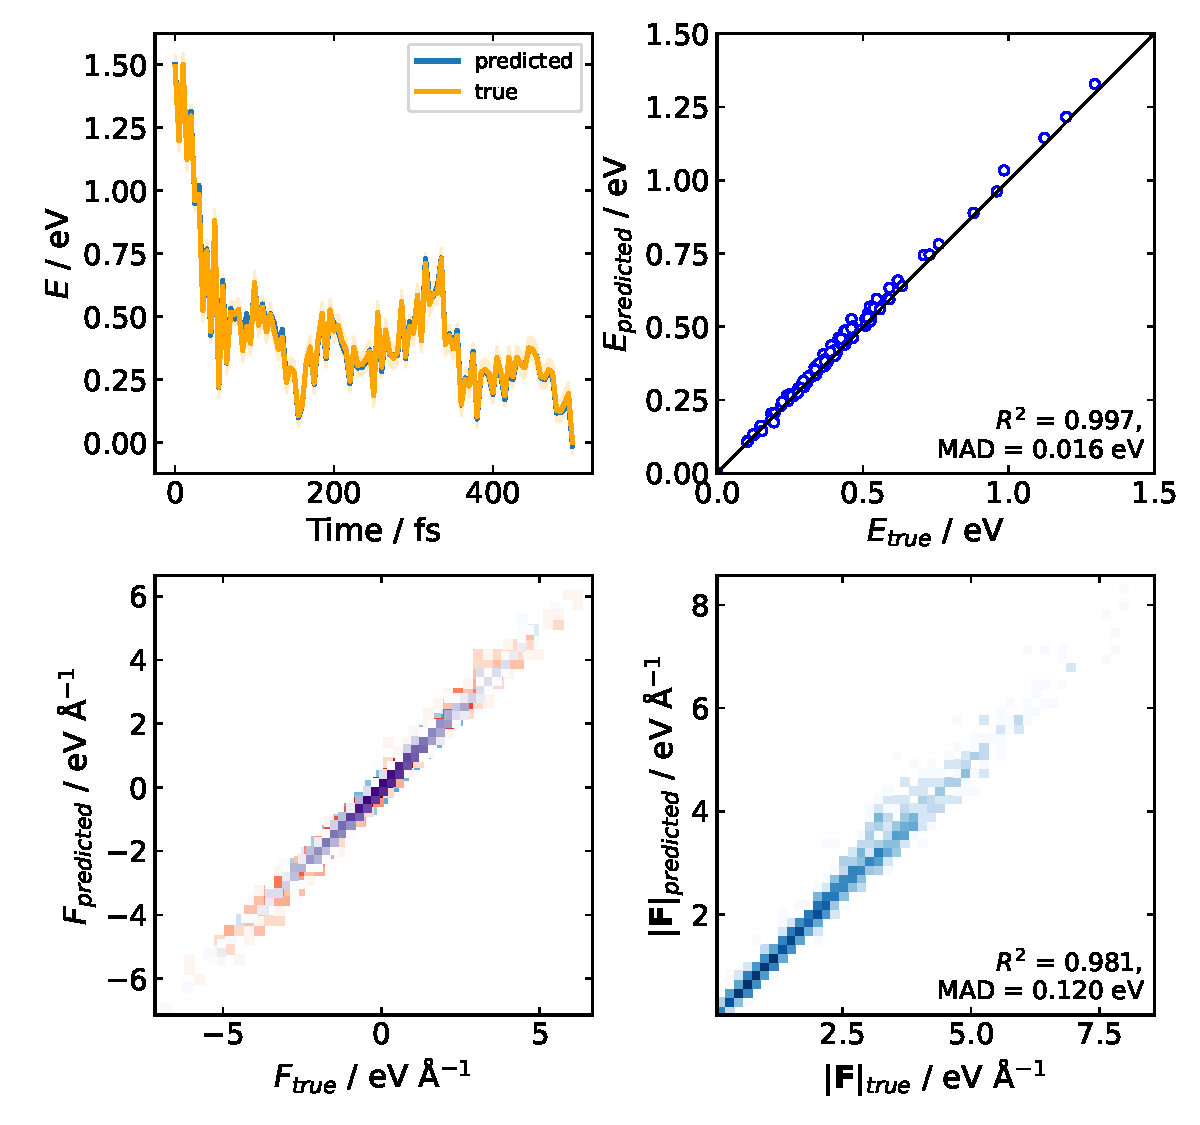
\includegraphics[height=11.2cm]{figSX38.pdf}
	\vspace{0.1cm}
	\hrule
	\vspace{0.1cm}
	\caption{Accuracy of an ACE potential on ACE-MD dynamics from the [4+2] TS between acetylene + cyclopentadiene. AL performed at 500 K for a maximum time of 1 ps per AL iteration and $E_T = 1$ \kcal. Converged training data contains 159 configurations. PBE0/def2-SVP level of theory.}
	\label{fig::SX38}
\end{figure}


\begin{figure}[h!]
	\centering
	\vspace{0.4cm}
	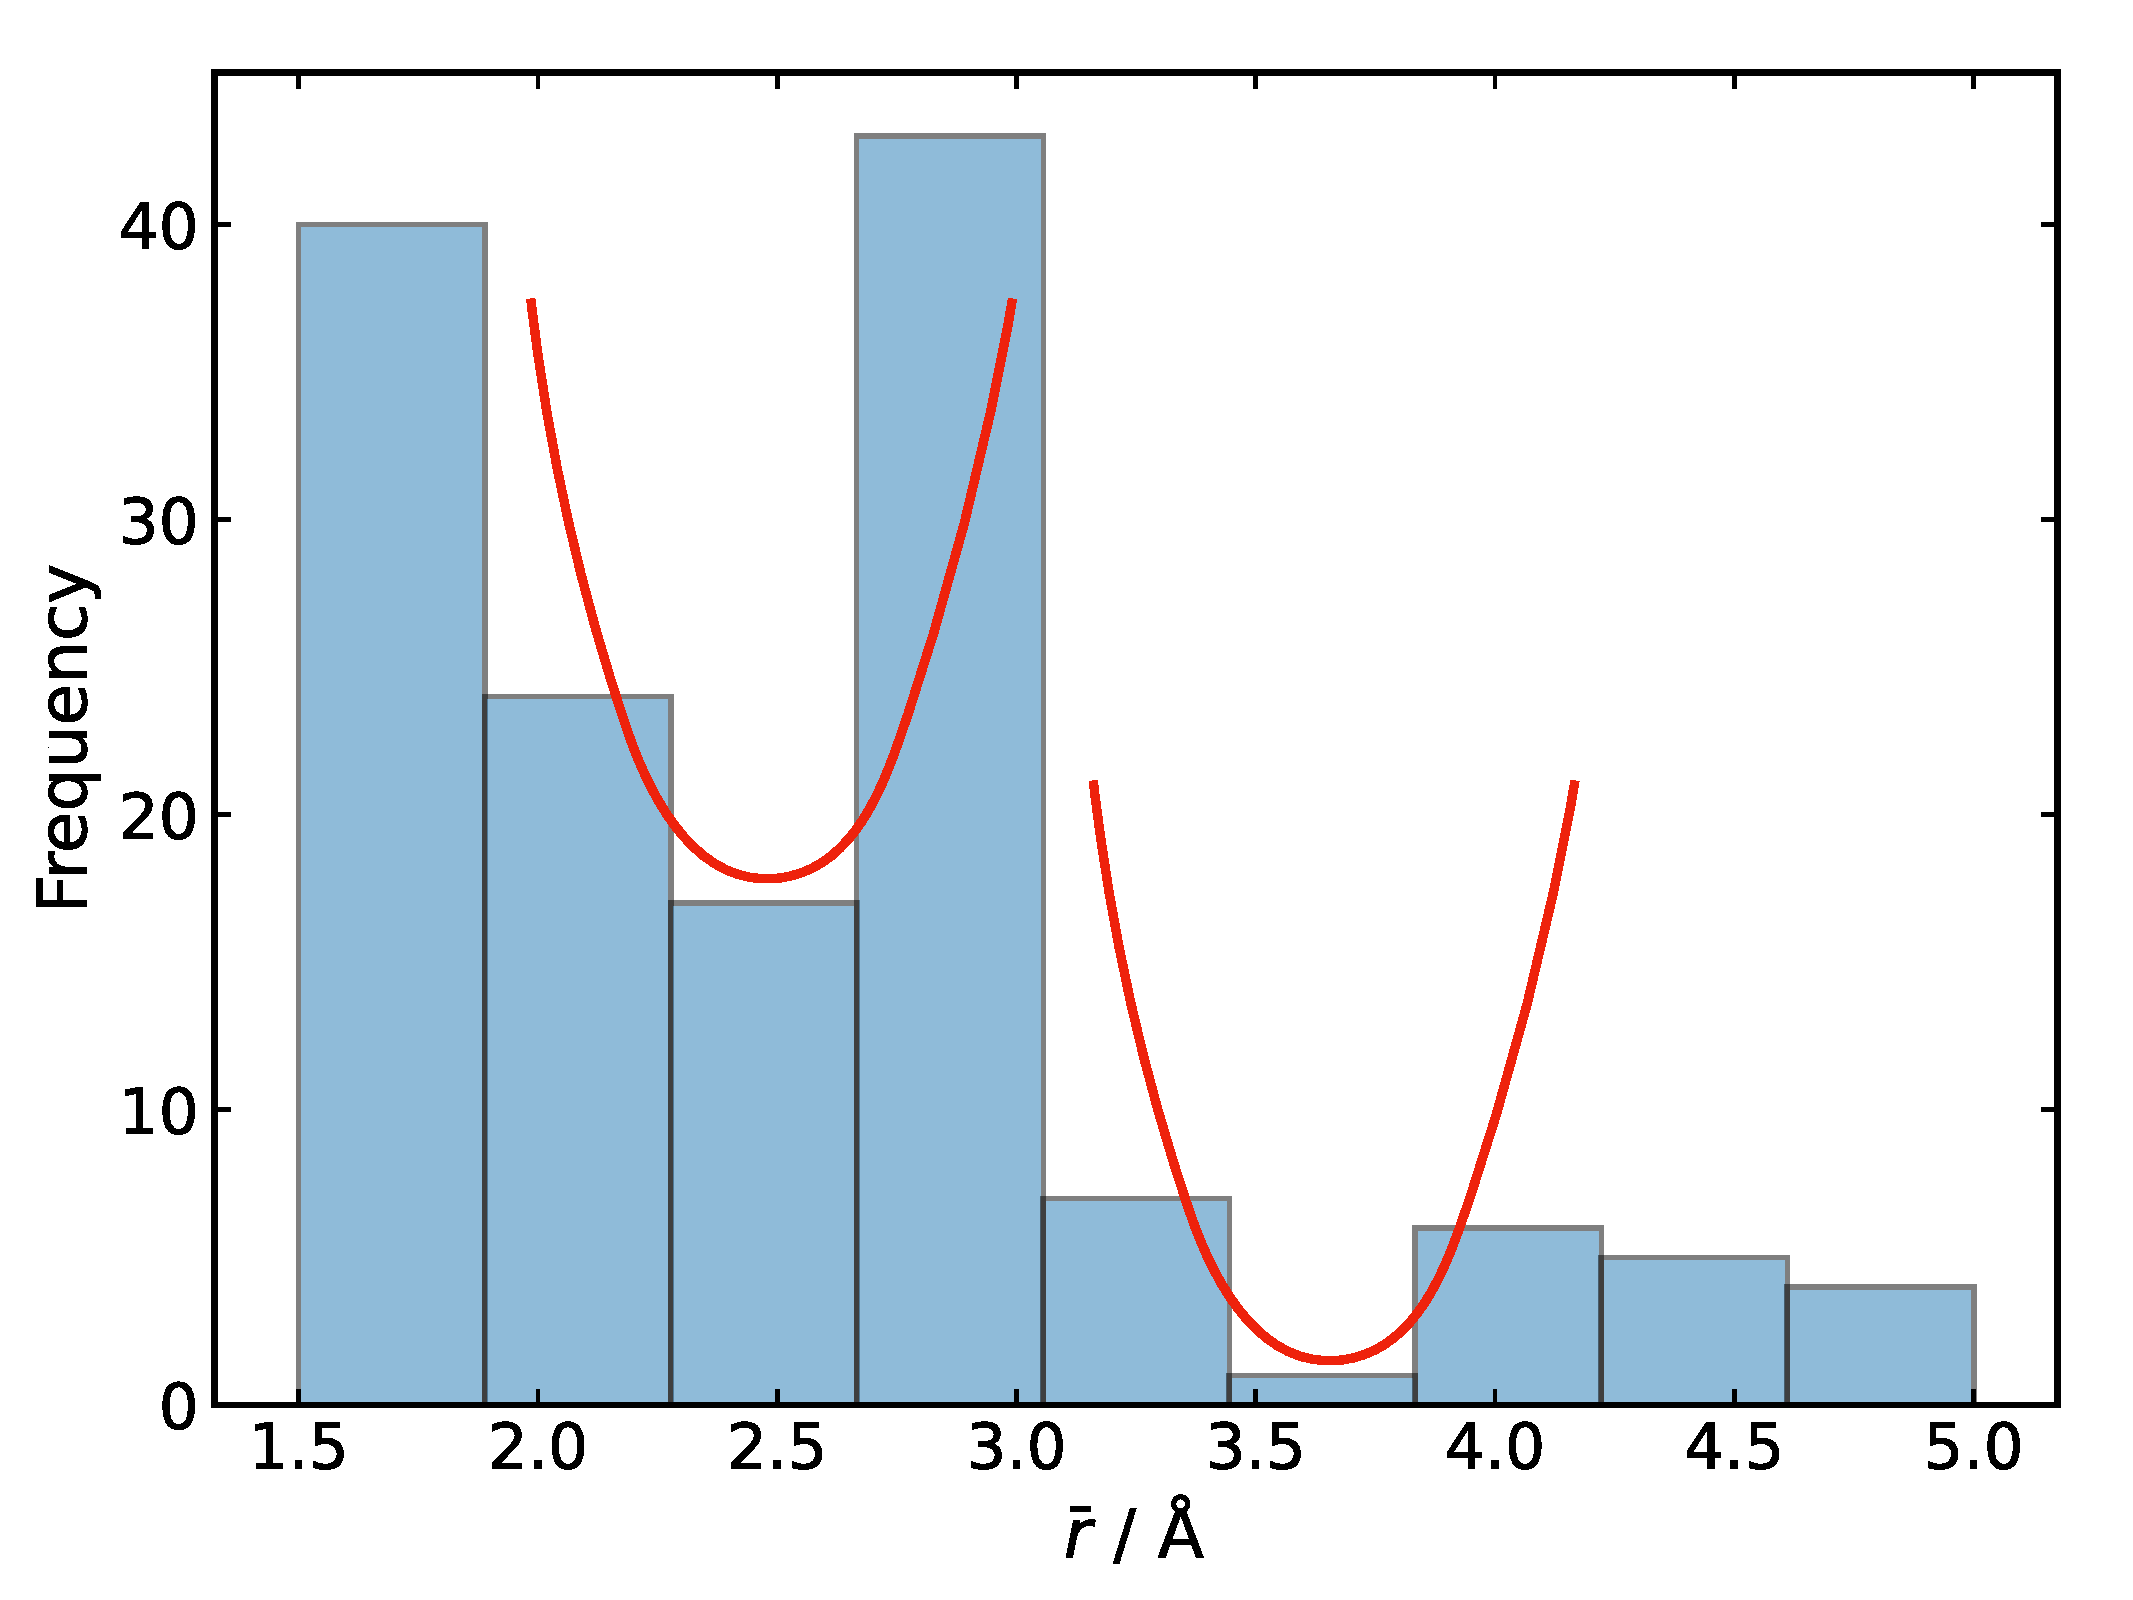
\includegraphics[height=6.4cm]{figSX39.pdf}
	\vspace{0.1cm}
	\hrule
	\vspace{0.1cm}
	\caption{Histogram of $\bar{r} = (r_1 + r_2) / 2$ for the DA reaction between acetylene + cyclopentadiene sampled in unbiased AL. Red harmonic potentials represent where additional biased sampling is performed following the unbiased AL terminating.}
	\label{fig::SX39}
\end{figure}



\begin{figure}[h!]
	\centering
	\vspace{0.4cm}
	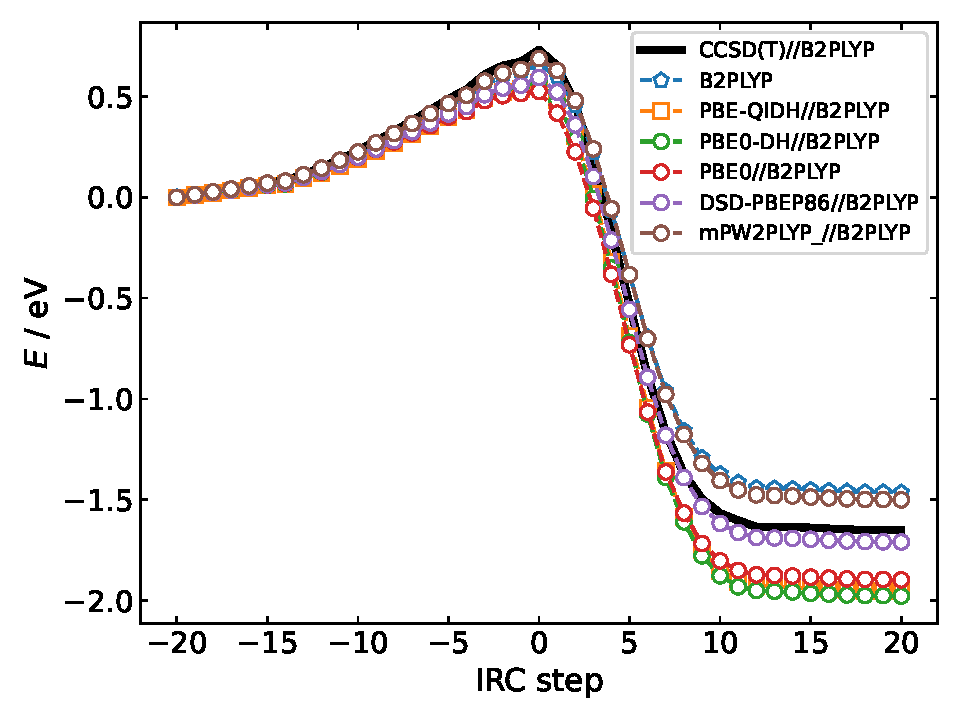
\includegraphics[height=6.4cm]{figSX32.pdf}
	\vspace{0.1cm}
	\hrule
	\vspace{0.1cm}
	\caption{Comparison of QM methods over the B2PLYP/def2-TZVP intrinsic reaction coordinate (IRC) incremented backwards and forwards from the B2PLYP/def2-TZVP [4+2] TS between acetylene + cyclopentadiene. All methods use the def2-TZVP basis set and resolution of the identity for MP2 and HF components.}
	\label{fig::SX32}
\end{figure}



\begin{figure}[h!]
	\centering
	\vspace{0.4cm}
	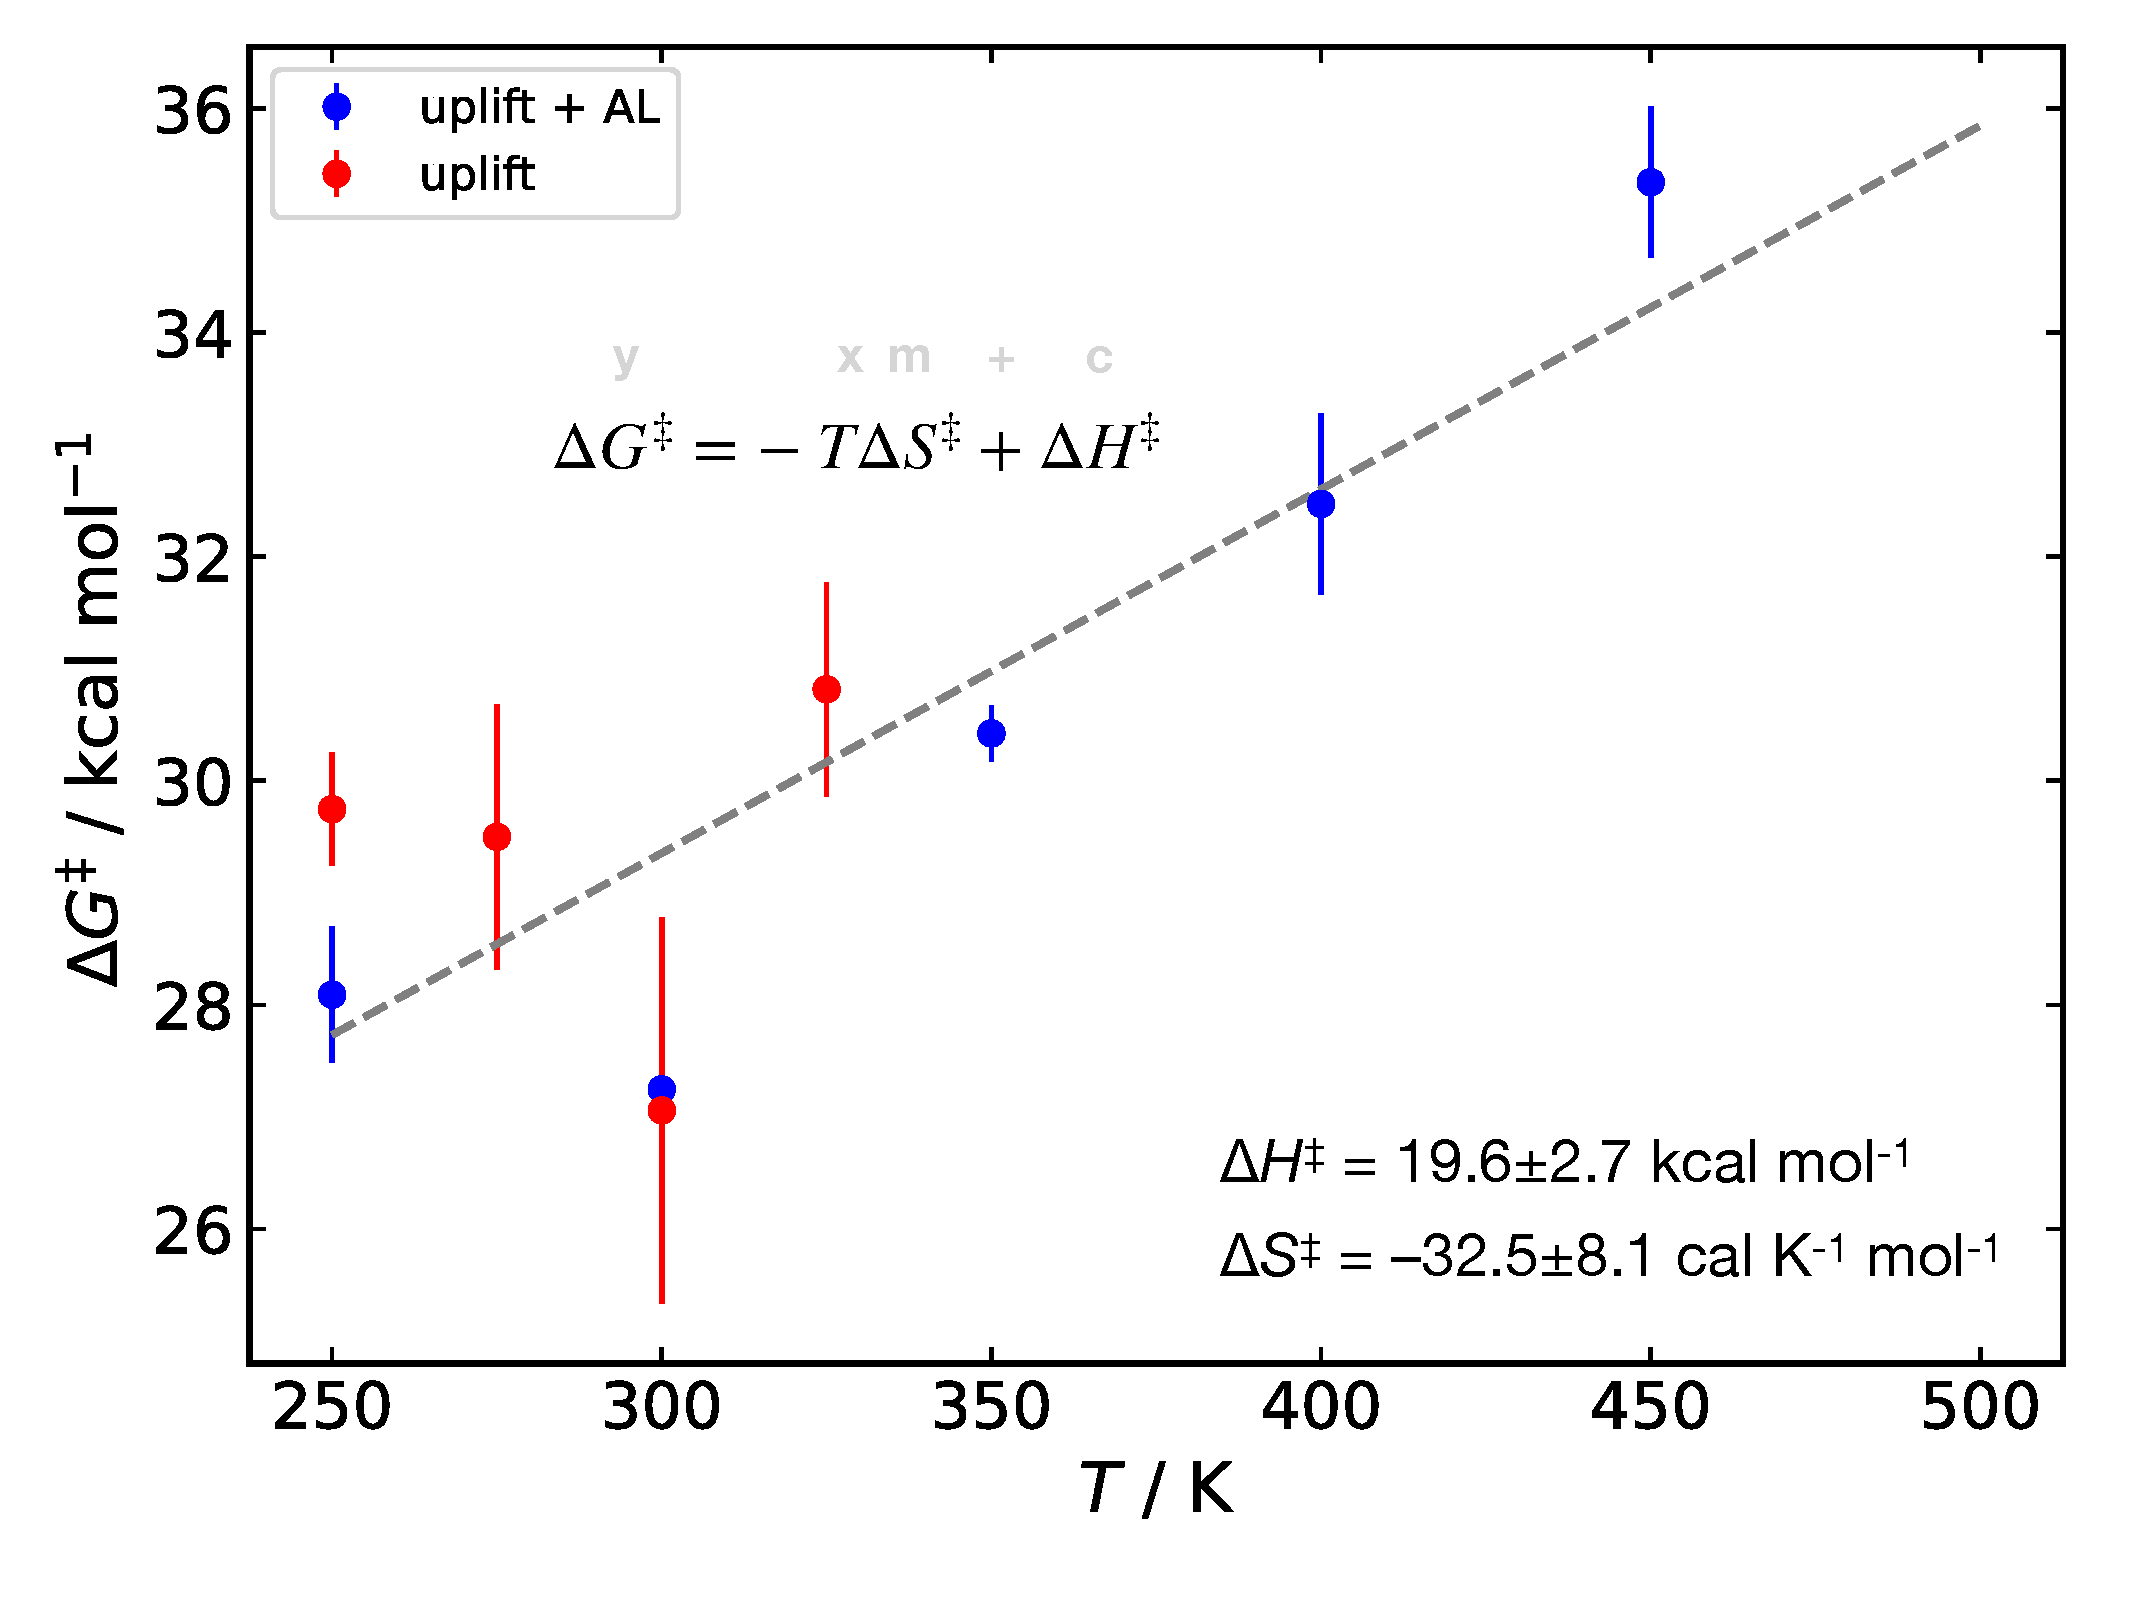
\includegraphics[height=6.4cm]{figSX37.pdf}
	\vspace{0.1cm}
	\hrule
	\vspace{0.1cm}
	\caption{Correlation between temperature and activation free energy from US simulations (as \figurename{ \ref{fig::SX36}}). Error bars are plotted as the standard error in the mean from three repeat simulations. Free energies include a correction from a simulation box of with side length 10 \AA to the required volume at 1 atm.\cite{General2010}}
	\label{fig::SX37}
\end{figure}


\begin{figure}[h!]
	\centering
	\vspace{0.4cm}
	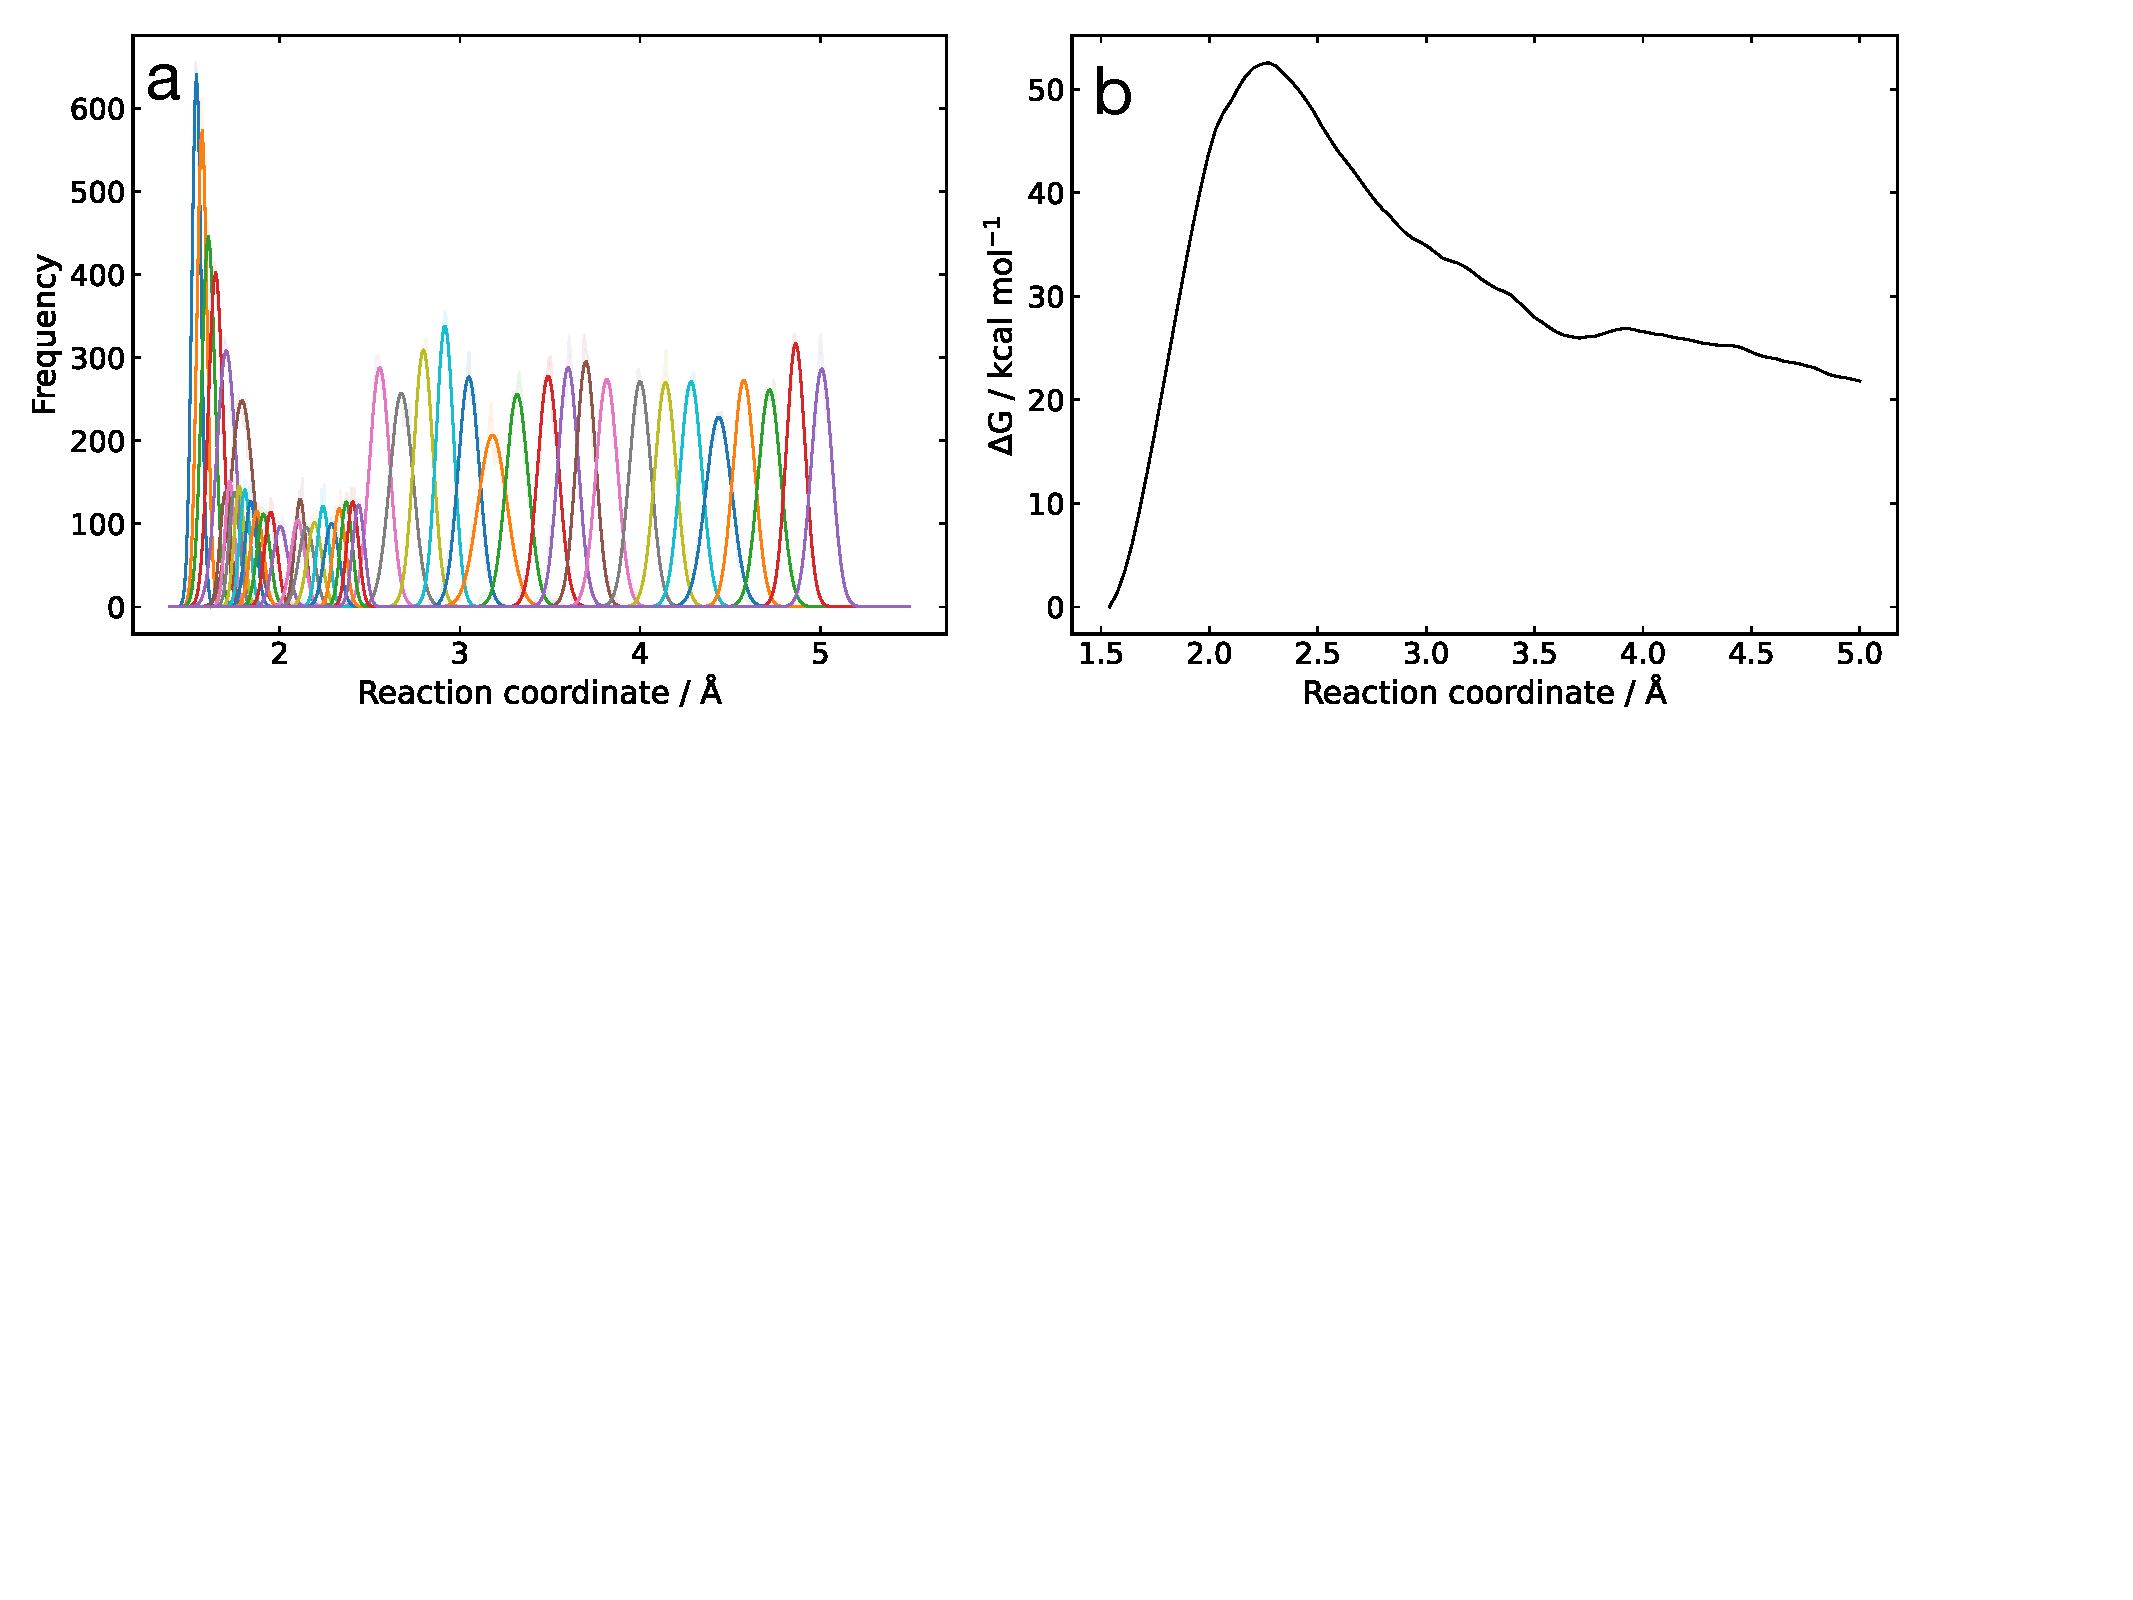
\includegraphics[height=6.4cm]{figSX36.pdf}
	\vspace{0.1cm}
	\hrule
	\vspace{0.1cm}
	\caption{Example of an umbrella sampling simulation. 450 K, 0.5 fs time step, 10 ps per window. 25 windows equally spaced in [1.539, 5.0] \AA with $k = 10$ eV \AA${}^{-1}$ and 10 equally spaced over [1.8, 2.4] \AA with $k = 40$ eV \AA${}^{-1}$. (a) Histogrammed reaction coordinate, defined by the average of the two forming bonds, for each umbrella containing a harmonic bias. (b) Free energy obtained from weighted histogram analysis (WHAM) unbiasing of the simulation; approximately equal to the potential of mean force (PMF).}
	\label{fig::SX36}
\end{figure}


\clearpage
\printbibliography

\end{document}
